%%%%%%%%%%%%%%%%%%%%%%%%%%%%%%%%%%%%%%%%%%%%%%%%%%%%%%%%%%%%%%%%%
%_____________ ___    _____  __      __ 
%\____    /   |   \  /  _  \/  \    /  \  Institute of Applied
%  /     /    ~    \/  /_\  \   \/\/   /  Psychology
% /     /\    Y    /    |    \        /   Zürcher Hochschule 
%/_______ \___|_  /\____|__  /\__/\  /    fuer Angewandte Wissen.
%        \/     \/         \/      \/                           
%%%%%%%%%%%%%%%%%%%%%%%%%%%%%%%%%%%%%%%%%%%%%%%%%%%%%%%%%%%%%%%%%
%
% Project     : Bachelorarbeit
% Title       : Auswirkung von Media-Multitasking auf das SWB
% File        : doc.tex Rev. 00
% Date        : 06.12.2013
% Author      : Till J. Ernst
%
%%%%%%%%%%%%%%%%%%%%%%%%%%%%%%%%%%%%%%%%%%%%%%%%%%%%%%%%%%%%%%%%%

%%%%%%%%%%%%%%%%%%%%%%%%%%%%%%%%%%%%%%%%%%%%%%%%%%%%%%%%%%%%%%%%%
%_____________ ___    _____  __      __ 
%\____    /   |   \  /  _  \/  \    /  \  Institute of Applied
%  /     /    ~    \/  /_\  \   \/\/   /  Psychology
% /     /\    Y    /    |    \        /   Zuercher Hochschule 
%/_______ \___|_  /\____|__  /\__/\  /    fuer Angewandte Wissen.
%        \/     \/         \/      \/                           
%%%%%%%%%%%%%%%%%%%%%%%%%%%%%%%%%%%%%%%%%%%%%%%%%%%%%%%%%%%%%%%%%
%
% Project     : Bachelorarbeit
% Title       : Header
% File        : header.tex Rev. 00
% Date        : 06.12.2013
% Author      : Till J. Ernst
%
%%%%%%%%%%%%%%%%%%%%%%%%%%%%%%%%%%%%%%%%%%%%%%%%%%%%%%%%%%%%%%%%%

\documentclass[
	appendixprefix,
	numbers=noenddot,
	oneside,
	12pt,
	parskip=half,
	ngerman,
	version=first
]{scrreprt}
%article scrartcl
%report scrreprt / report
%book scrbook
%letter scrlttr2

%***********************************************************************
% include some libs
%***********************************************************************	
\usepackage[utf8]{inputenc}
\usepackage[T1]{fontenc}
\usepackage{textcomp}
\usepackage{listings}
\usepackage{color}
\usepackage{fancyhdr}
\usepackage{rotating}
\usepackage{titlesec}
\usepackage{mathptmx} 
\usepackage[scaled=.90]{helvet}
%\usepackage{courier}
\usepackage[urw-garamond]{mathdesign}
\usepackage{setspace} %Zeilenabstand
\onehalfspacing % 1,5 Zeilenabstand
%\renewcommand*\familydefault{\sfdefault} %% Only if the base font of the document is to be sans serif
%\usepackage{german}
\usepackage[]{ragged2e}
\usepackage[ngerman]{babel}
%\usepackage[babel]{csquotes}
\usepackage[squaren]{SIunits}
\usepackage{graphicx}
\usepackage{url}
\usepackage[a4paper]{geometry}
\usepackage[absolute]{textpos}
\usepackage{makeidx}
\usepackage{colortbl}
\usepackage{pdflscape}
\usepackage{pdfpages}
\usepackage{tabularx}
\usepackage{lmodern}
\usepackage{longtable}
\usepackage{multirow}
\usepackage{array}
\usepackage{float}
\usepackage{scrhack}
\usepackage{wallpaper}
\usepackage{titleref}
\usepackage{tocloft} % fancy TOC

% Bereitstellung Hyperlinkfunktionen (PDF) (muss als letztes Paket geladen werden)
\usepackage[
	colorlinks=true,
	breaklinks=true,
	linkcolor=black,
	citecolor=black,
	urlcolor=black,
	anchorcolor=black,
	pdfpagelabels,
	pdftitle={Beeinflusst Multitasking das eigene Glück},
	pdfsubject={Die Auswirkungen von Medien-Multitasking auf das subjektive Wohlbefinden von Studierenden},
	pdfkeywords={KEYWORDS},
	pdfauthor={Till J. Ernst (ernsttil)}
]{hyperref}

%Biblatex APA 6 Style
\usepackage{apacite}

%\usepackage[american]{babel}
%\usepackage{csquotes}
%\usepackage[
%    style=apa,
%    backend=biber
%]{biblatex}
%\DeclareLanguageMapping{german}{german-apa}
%\addbibresource{Bibliography.bib}

% Bereitstellen Anhang
\usepackage[toc,page]{appendix}

% Bereitstellung Glossar
\usepackage[acronym]{glossaries}
\makeglossaries





%***********************************************************************
% various styles
%**********************************************************************
%create index
\makeindex

%define pagestyle
\pagestyle{fancy}

%use sans-serif font 
%\renewcommand{\familydefault}{\sfdefault}

%define page margin
\geometry{a4paper, top=25mm, left=25mm, right=25mm, bottom=25mm,headsep=10mm,footskip=10mm}

%textpos parameter
\setlength{\TPHorizModule}{30mm}
\setlength{\TPVertModule}{\TPHorizModule}
\textblockorigin{10mm}{10mm} % start everything near the top-left corner
%The \setlength command is used to set the value of a length command, len-cmd, which is specified as the first argument.
\setlength{\headheight}{28pt}
\setlength{\parindent}{0pt} % Bei Absatz neuer Einzug

%horizontal lines for titlepage 
\newcommand{\HRule}{\rule{\linewidth}{0.5mm}}

%reference to source items inlc source number
\newcommand{\srcref}[1]{\nameref{src:#1} \cite{#1}}

% Umdefinieren des Layouts (otional)
% - - - - - - - - - -
\fancyhf{} %alle Kopf- und Fußzeilenfelder bereinigen
%\fancyhead[OR,EL]{\rightmark} %die Section-Name
\fancyhead[L]{\leftmark} % Chapter-Name
%\fancyhead[OL,ER]{\leftmark} % Chapter-Name -> nur nötig bei 2 Seiten Layout
\renewcommand{\headrulewidth}{0.3pt}
\fancyfoot[C]{\textbf \Large \thepage} 
\renewcommand{\footrulewidth}{0pt}
\renewcommand{\arraystretch}{1.5} % für tabellen

%\fancyhead[LO,RE]{} %clear headings for contents 
%\fancyhead[RO,LE]{\nouppercase{\rightmark}} %right odd pages and left even pages
%\fancyhead[LO,RE]{\MakeUppercase{\leftmark}} %left odd pages and right even pages
%\fancyfoot[LE,RO]{\thepage} %page numbering
%\fancyfoot[C]{} %clear centered page numbering 

%define some colors
\definecolor{gray}{rgb}{0.95,0.95,0.95}
\definecolor{darkgray}{rgb}{0.4,0.4,0.4}
%listing colors
\definecolor{lgray}{RGB}{250,250,250}
\definecolor{lgreen}{RGB}{63,127,95}
\definecolor{lred}{RGB}{127,0,85}
\definecolor{lblue}{RGB}{42,0,255}

% Für Tabellen: Textausrichtung bei fester Spaltenbreite
\newcolumntype{L}[1]{>{\raggedright\arraybackslash}p{#1}} % linksbündig mit Breitenangabe
\newcolumntype{C}[1]{>{\centering\arraybackslash}p{#1}} % zentriert mit Breitenangabe
\newcolumntype{R}[1]{>{\raggedleft\arraybackslash}p{#1}} % rechtsbündig mit Breitenangabe


%***********************************************************************
% listing
%***********************************************************************

\lstset{		
		basicstyle=\small\ttfamily,
		frame=single,
		numbers=left,	
		numberstyle=\tiny,
		%firstnumber=auto,
		numberblanklines=true,
		captionpos=b,
		extendedchars=true,
		float=ht,
		showtabs=false,
		tabsize=2,
		showspaces=false,
		showstringspaces=false,
		breaklines=true,
		%prebreak=\Righttorque,
		backgroundcolor=\color{lgray},
		keywordstyle=\color{lred}\bfseries, 
		commentstyle=\color{lgreen}\ttfamily,
%		morekeywords={printstr, printhexln},
		stringstyle=\color{lblue},
		xleftmargin=0.5cm,
		xrightmargin=0.5cm
}


\begin{document}
\title{Die Auswirkung von Medien-Multitasking auf das subjektive Wohlbefinden von Studierenden}
\author{Till J. Ernst}

%PDF Titelblatt
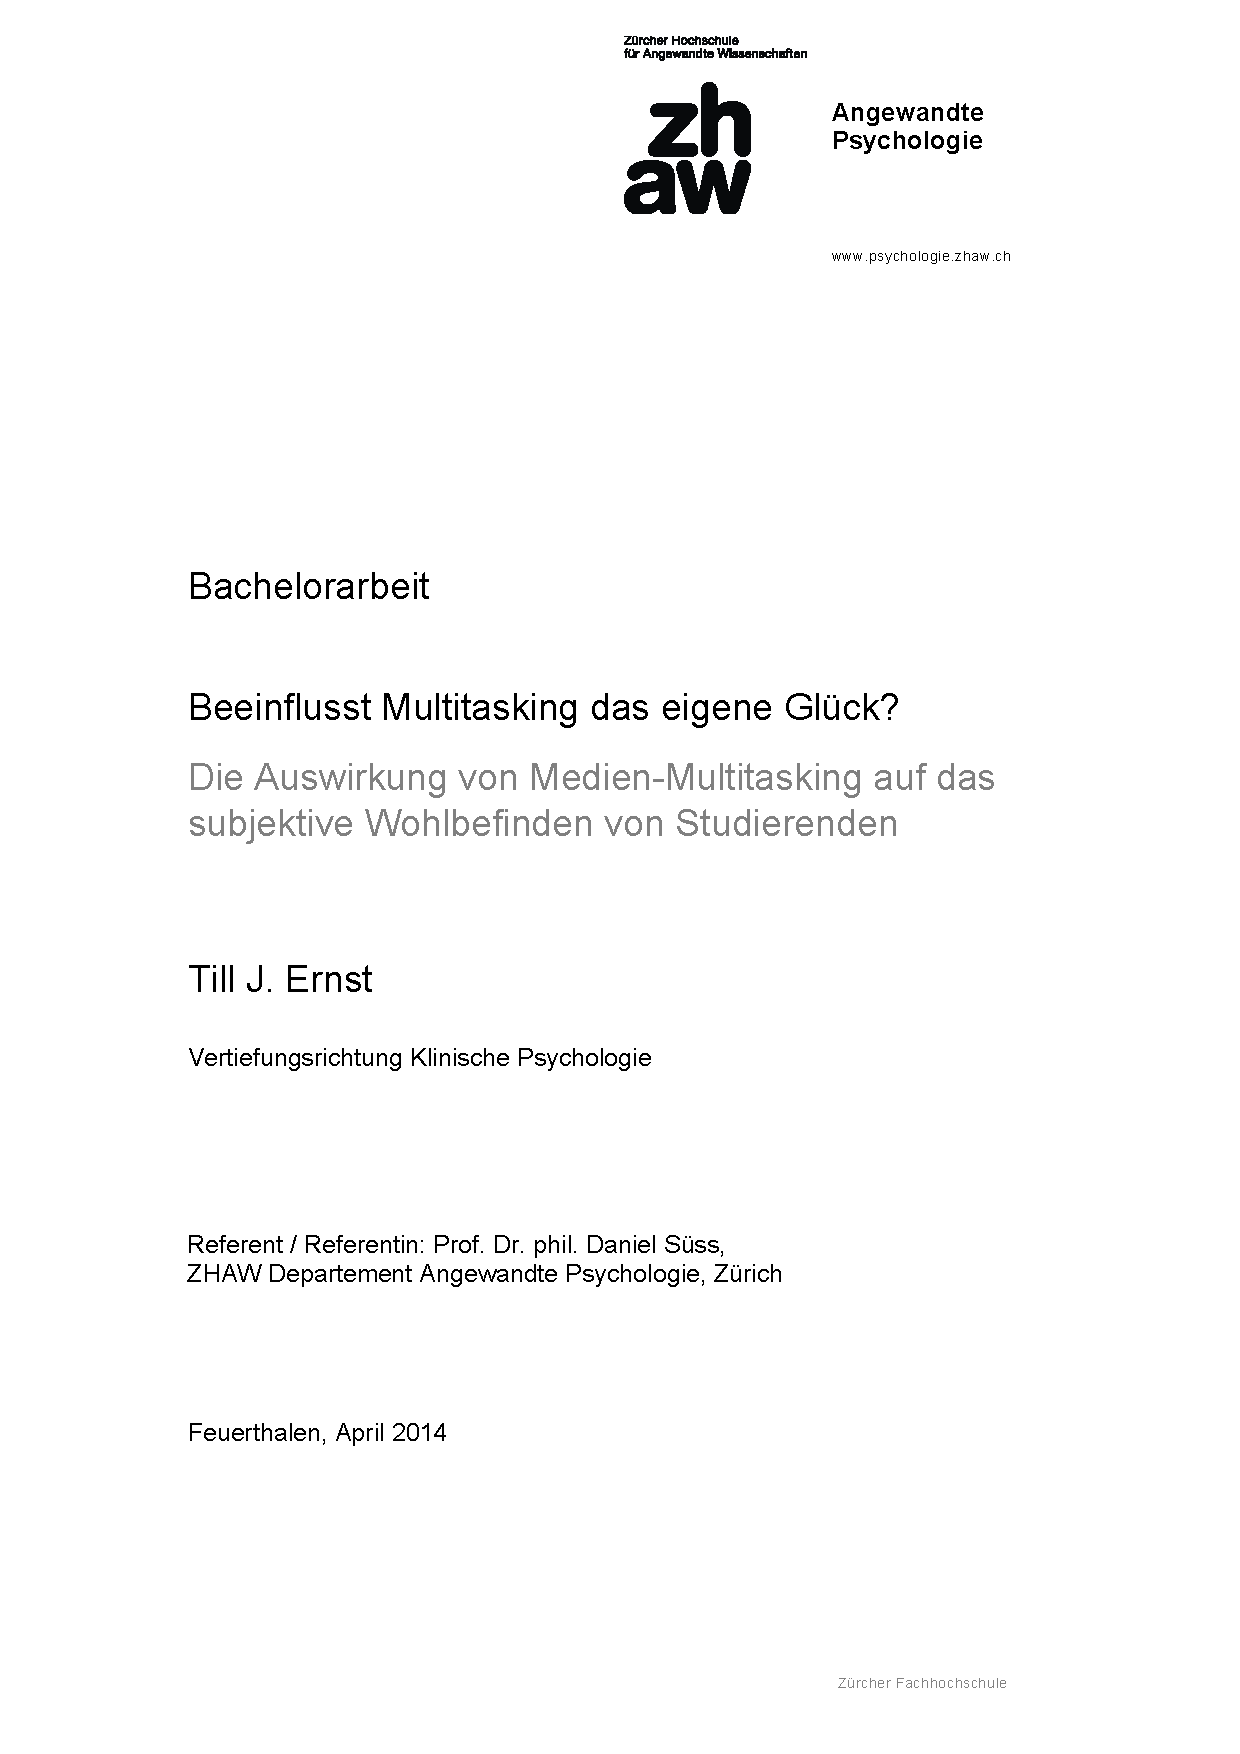
\includepdf{images/Bachelorarbeit_Titelblatt.pdf}

%PDF Bestimmungsblatt

\includepdf{images/Bachelorarbeit_Bestimmungen.pdf}

% -> Keine Seitenzahlen bis TOC
\pagenumbering{gobble} 

% Danksagung
%\begin{RaggedRight}
%%%%%%%%%%%%%%%%%%%%%%%%%%%%%%%%%%%%%%%%%%%%%%%%%%%%%%%%%%%%%%%%%
%_____________ ___    _____  __      __ 
%\____    /   |   \  /  _  \/  \    /  \  Institute of Applied
%  /     /    ~    \/  /_\  \   \/\/   /  Psychology
% /     /\    Y    /    |    \        /   Zuercher Hochschule 
%/_______ \___|_  /\____|__  /\__/\  /    fuer Angewandte Wissen.
%        \/     \/         \/      \/                           
%%%%%%%%%%%%%%%%%%%%%%%%%%%%%%%%%%%%%%%%%%%%%%%%%%%%%%%%%%%%%%%%%
%
% Project     : Bachelorarbeit
% Title       : Danksagung
% File        : danksagung.tex Rev. 00
% Date        : 06.12.2013
% Author      : Till J. Ernst
%
%%%%%%%%%%%%%%%%%%%%%%%%%%%%%%%%%%%%%%%%%%%%%%%%%%%%%%%%%%%%%%%%%
\thispagestyle{empty} 
\let\raggedsection\centering
\chapter*{Danksagung}\label{label.danksagung}
\let\raggedsection\raggedright 
TBD

% Vorwort
%%%%%%%%%%%%%%%%%%%%%%%%%%%%%%%%%%%%%%%%%%%%%%%%%%%%%%%%%%%%%%%%%
%_____________ ___    _____  __      __ 
%\____    /   |   \  /  _  \/  \    /  \  Institute of Applied
%  /     /    ~    \/  /_\  \   \/\/   /  Psychology
% /     /\    Y    /    |    \        /   Zuercher Hochschule 
%/_______ \___|_  /\____|__  /\__/\  /    fuer Angewandte Wissen.
%        \/     \/         \/      \/                           
%%%%%%%%%%%%%%%%%%%%%%%%%%%%%%%%%%%%%%%%%%%%%%%%%%%%%%%%%%%%%%%%%
%
% Project     : Bachelorarbeit
% Title       : Vorwort
% File        : vorwort.tex Rev. 00
% Date        : 06.12.2013
% Author      : Till J. Ernst
%
%%%%%%%%%%%%%%%%%%%%%%%%%%%%%%%%%%%%%%%%%%%%%%%%%%%%%%%%%%%%%%%%%
\thispagestyle{empty} 
\let\raggedsection\centering
\chapter*{Vorwort}\label{label.vorwort}
\let\raggedsection\raggedright 
TBD

% Abstract
%%%%%%%%%%%%%%%%%%%%%%%%%%%%%%%%%%%%%%%%%%%%%%%%%%%%%%%%%%%%%%%%%
%_____________ ___    _____  __      __ 
%\____    /   |   \  /  _  \/  \    /  \  Institute of Applied
%  /     /    ~    \/  /_\  \   \/\/   /  Psychology
% /     /\    Y    /    |    \        /   Zuercher Hochschule 
%/_______ \___|_  /\____|__  /\__/\  /    fuer Angewandte Wissen.
%        \/     \/         \/      \/                           
%%%%%%%%%%%%%%%%%%%%%%%%%%%%%%%%%%%%%%%%%%%%%%%%%%%%%%%%%%%%%%%%%
%
% Project     : Bachelorarbeit
% Title       : Abstract
% File        : abstract.tex Rev. 00
% Date        : 06.12.2013
% Author      : Till J. Ernst
%
%%%%%%%%%%%%%%%%%%%%%%%%%%%%%%%%%%%%%%%%%%%%%%%%%%%%%%%%%%%%%%%%%
\thispagestyle{empty} 
\chapter*{Abstract}\label{abstract}
\textbf{Hintergrund:} TBD 
\par 
\textbf{Methoden:} TBD 
\par 
\textbf{Resultate:} TBD
\par 
\textbf{Schlussfolgerung:} TBD 


 

% Inhaltsverzeichnis
\setcounter{page}{1}
\pagenumbering{Roman}
\renewcommand*\contentsname{\hfill Inhalt \hfill}
\tableofcontents
\newpage

% Abbildungsverzeichnis
%\def\listfigurename{\centerline{\textbf{\large{Abbildungsverzeichnis}}}} 
\listoffigures
\newpage

% Tabellenverzeichnis
\listoftables
\newpage

% Abkürzungsverzeichnis
% Examples
% \gls{<label>}

% ###################################################
% List of Acronyms
% ###################################################
\newacronym{labelPRP}{PRP}{Psychologische Refraktaerperiode}
\newacronym{labelSWB}{SWB}{Subjektive Wohlbefinden}
\newacronym{labelMT}{MT}{Multitasking}
\newacronym{labelMMT}{MMT}{Medien-Multitasking}
\newacronym{labelMMI}{MMI}{Media-Multitasking-Index}
\newacronym{labelMUQ}{MUQ}{Media Use Questionnaire}
\newacronym{labelACS}{ACS}{Attentional Control Scale}
\newacronym{labelFS}{FS}{The Flourishing Scale}
\newacronym{labelSPANE}{SPANE}{The Scale of Positive and Negative Epxerience}
\glossarystyle{altlist}
\printglossary[title=Abkürzungsverzeichnis]
\glsaddall % If all entries are to be printed the command
\newpage

%%%%%%%%%%%%%%%%%%%%%%%%%%%%%%%%%%%%%%%%%%%%%%%%%%%%%%%%%%%%% 
%% Hauptteil
%%%%%%%%%%%%%%%%%%%%%%%%%%%%%%%%%%%%%%%%%%%%%%%%%%%%%%%%%%%%%
% Kapitel
% -----------------------------------
\setcounter{page}{1}
\pagenumbering{arabic}
% Einleitung
%%%%%%%%%%%%%%%%%%%%%%%%%%%%%%%%%%%%%%%%%%%%%%%%%%%%%%%%%%%%%%%%%
%_____________ ___    _____  __      __ 
%\____    /   |   \  /  _  \/  \    /  \  Institute of Applied
%  /     /    ~    \/  /_\  \   \/\/   /  Psychology
% /     /\    Y    /    |    \        /   Zuercher Hochschule 
%/_______ \___|_  /\____|__  /\__/\  /    fuer Angewandte Wissen.
%        \/     \/         \/      \/                           
%%%%%%%%%%%%%%%%%%%%%%%%%%%%%%%%%%%%%%%%%%%%%%%%%%%%%%%%%%%%%%%%%
%
% Project     : Bachelorarbeit
% Title       : Einleitung
% File        : einleitung Rev. 00
% Date        : 06.12.2013
% Author      : Till J. Ernst
%
%%%%%%%%%%%%%%%%%%%%%%%%%%%%%%%%%%%%%%%%%%%%%%%%%%%%%%%%%%%%%%%%%
\glsresetall % zurücksetzen der Acronyms
\chapter{Einleitung (Gegenwart)}\label{chap.einleitung}

%####################################################
% Kapitel Ausgangslage
%####################################################
\section{Ausgangslage}\label{section.einleitung.ausgangslage}
Die leichte Zugänglichkeit von Medien über neue Technologien wie Smartphones, Tablets und Computer hat den Medienkonsum rasant ansteigen lassen. Zum Beispiel konnte in der gross angelegten Studie der Kaiser Family Foundation \cite{Rideout2010} von über 2000 8- bis 18-Jährigen festgestellt werden, dass die Gesamtzeit, in der die Jugendlichen den Medien ausgesetzt sind, im Jahr 2009 auf 10 Stunden und 45 Minuten pro Tag angestiegen ist. Im Jahr 2004 waren es noch 8 Stunden und 33 Minuten und 1999 7 Stunden und 29 Minuten. Dies entspricht einem Anstieg von 44\% innerhalb von einem Jahrzehnt. Die eigentliche Mediennutzung stieg von 6 Stunden und 19 Minuten im Jahr 1999 auf 7 Stunden und 38 Minuten im Jahr 2009 an. Diese entspricht beinahe der Arbeitszeit, die Erwachsenen pro Tag auf der Arbeit verbringen \cite{Rideout2010}. In der Schweiz gehören digitale Medien zu den beliebtesten Freizeitaktivitäten der Jugendlichen. Dazu gehören Medien wie das Mobiltelefon, Internet und Musik hören. Wobei das Mobiltelefon das am meisten genutzte Medium darstellt \cite{Willemse2012}. Die universelle Medienbenützung wird zu einem globalen Phänomen. Nicht nur jugendliche sind von diesem Trend betroffen, vielmehr handelt es sich hierbei um eine Entwicklung, die in allen Altersgruppen und Berufsgruppen anzutreffen ist \cite{Rogers2009}. Diese Mediennutzung hat längst Einzug in unseren Arbeitsstätten und Klassenräumen gehalten und hat uns ein Stückweit den Weg gewiesen, wie wir untereinander Kommunizieren und interagieren \cite{Benson2002}. Dieser rasante Anstieg der Mediennutzung lässt die Frage nach möglichen Auswirkungen des enormen Medien-Konsums auf die psychische Gesundheit und kognitive Funktion entstehen. Aktuelle Forschungsergebnisse lassen jedoch noch keinen eindeutigen Schluss auf diese Frage zu. Einführende Studien deuten darauf hin, dass sich die Befürchtung einer Verschlechterung der Psyche und der Hirnfunktionen bewahrheitet \cite{Biocca2000, Roberts2008}. Im Forschungsbereich der psychischen Gesundheit wurden Anzeichen für einen Zusammenhang zwischen Medienkonsum und negativ einhergehendem sozialem Wohlbefinden und verminderten psychosozialen Funktionen gefunden \cite{Kraut1998, Moody2001}. Im Bildungsbereich wurden Anzeichen für einen möglichen Medien-Einfluss auf das Lernverhalten festgestellt \cite{Prensky2001}. In den meisten bisherig erwähnten Forschungsergebnissen wurde das Ausmass anhand der eigentlichen Medien-Nutzungsdauer untersucht. Dabei spielt das simultane Benützen mehrerer Medien eine immer grösser werdende Rolle. Währendem die absolute Nutzungsdauer in den vergangenen Jahren rapide angestiegen ist, so konnte bei dieser Art von Mediennutzung erst recht eine Steigerung festgestellt werden. Im letzten Jahrzehnt hat sich das Verhältnis von Medien-Multitasking (das gleichzeitige Benutzen mehrere Medien) gegenüber der eigentlichen Mediennutzung von 16\% in 1999 auf 29\% in 2009 gesteigert \cite{Rideout2010}. Dieser rasante Anstieg lässt erneut Fragen betreffend Auswirkungen auf die Gedächtnisleistung und die psychische Gesundheit entstehen \cite{Alzahabi2013}. 

%####################################################
% Kapitel Hintergrund, Begründung und Ziel der Studie
%####################################################
\section{Hintergrund, Begründung und Ziel der Studie}\label{section.einleitung.hintergrund}
Ausgehend von den wenig bereits existierenden Studien über die Auswirkungen von Medien-Multitasking geht hervor, dass Medien-Multitasking einmalig im Bezug zu den Auswirkungen auf psychische Gesundheit und kognitive Funktionen sei. Eine aktuelle Studie legt nahe, dass Medien-Multitasking mit höheren Symptomen von Depression und sozialer Angst einhergeht \cite{Becker2013} und mit ansteigendem Medien-Konsum und Multitasking nimmt das soziale Wohlbefinden von Mädchen ab \cite{Pea2012}. Bezüglich kognitiven Prozessen konnten negative Auswirkungen von Multitasking auf die Schulleistung gefunden werden \cite{Junco2012}. In einem Laborversuch von \citeA{Ophir2009} konnte ein Zusammenhang mit Medien-Multitasking und kognitiver Leistung nachgewiesen werden. Diese Studie legt nahe, dass starke Medien-Multitasker Mühe haben, zwischen einzelnen Aufgaben hin und her zu wechseln. Diese Multitasker mussten mehr Leistung für diesen Wechsel aufwenden, als moderate oder schwache Medien-Multitasker. Eine mögliche Erklärung für dieses Ergebnis könnte sein, dass das häufige Praktizieren von Medien-Multitasking die Fähigkeit der Nutzer für das simultane Verarbeiten von Informationen steigert, indes dafür die Notwendigkeit vom Wechsel zwischen Aufgaben verringert und somit die Übung für diesen Wechsel bei starken Multitasker ausbleibt \cite{Alzahabi2013, Watson2010}. Die Auswirkung von Medien-Multitasking auf die kognitiven Funktionen wurden in einigen Studien untersucht. Die Auswirkungen von Medien-Multitasking auf das subjektive Wohlbefinden hingegen, ist in der aktuellen Forschung bisweilen wenig vertreten. Eine aktuelle Studie um \citeA{Shih2013} mit 138 Studenten konnte keinen relevanten Zusammenhang zwischen Medien-Multitasking und dem Wohlbefinden herstellen. Trotz diesem Ergebnis ist klar, dass hier weitere Studien folgen müssen. Das Ziel dieser Bachelorarbeit ist es, einen Teil dieser Forschungslücke zu schliessen. Es soll die Auswirkung von Medien-Multitasking auf das subjektive Wohlbefinden näher untersucht und beleuchtet werden. Ein weiteres Ziel dieser Arbeit ist es, weitere Hinweise auf die kognitive Komponente im Zusammenhang mit Medien-Multitasking zu finden und zu analysieren. 

%####################################################
% Kapitel Aufbau der Arbeit
%####################################################
\section{Aufbau der Arbeit}\label{section.einleitung.aufbau}
Diese Arbeit beginnt mit einem einleitenden Kapitel, in dem theoretische Konstrukte und der aktuelle Forschungstand erläutert werden. Darin werden die Begriffe Multitasking und subjektives Wohlbefinden mit den für diese Arbeit weiteren relevanten Konstrukten erklärt. Aktuelle Forschungsergebnisse sollen weiter in die Thematik verhelfen und mögliche Forschungslücken aufzeigen. Abschliessend wird die Forschungsfrage und die daraus resultierende Hypothese hergeleitet. Im Methodenteil folgen Angaben über das eigentliche Studiendesign, die Auswahl der Stichprobe und die verwendeten Messmittel, um den daraus resultierenden Online-Fragebogen zu erstellen. Weiter wird die eigentliche Datenerhebung, die Datenaufbereitung und die dazu notwendigen statistischen Verfahren erläutert. Die Ergebnisse werden anhand der gefundenen Daten dargestellt und gemäss einleitender Hypothesen wiedergegeben und Analysiert.\\
Im Abschliessenden Teil dieser Arbeit werden die Ergebnisse in Bezug zu den Fragestellungen gesetzt und interpretiert. Es folgt eine Methodenkritik und einen Ausblick für weiterführende Untersuchungen.

%####################################################
% Kapitel Theoretischer Hintergrund
%####################################################
\section{Theoretischer Hintergrund}\label{section.einleitung.theoHintegrund}
Der theoretische Hintergrund dient zur Erläuterung von Begriffen, Konstrukten und Definitionen, auf denen diese Arbeit aufgebaut ist. In einem ersten Teil werden Begriffsbestimmungen und Definitionen behandelt. Anschliessend werden die beiden Konstrukte Medien-Multitasking und subjektives Wohlbefinden ausführlich erläutert. Diese Konstrukte bilden aus theoretischer Sicht die beiden Schwerpunkte dieser Arbeit.
% Begriffsbestimmungen, Definitionen ---------------------
\subsection{Begriffsbestimmungen, Definitionen}
\label{subsection.begriffsbestimmung}
\textbf{Sensation Seeking:}
Die Suche nach starken Reizen, wie dieses Konzept von \citeA{Zuckerman2006} auch umschrieben wird. Es geht hierbei um die Suche nach Abwechslung und neuen Erlebnissen. Streben nach starken Reizen und stimulierenden Erfahrungen, um Spannungsreize zu erleben. Diese Verhaltensdisposition basiert auf genetischer und biochemischer Basis. Dieses Konstrukt geht auf Freuds Konzept der Trieb oder Spannungsreduktion sowie auf das Modell der optimalen Stimulation und Erregung zurück \cite{Doernhaus2014}. 
\par
\textbf{Digital Natives und Digital Immigrants:} Im Umgang mit Medien und der daraus resultierenden Medienkompetenz wird oft anhand der Generationsgestaltung eine Unterteilung nach Alterskohorten vorgenommen \cite{Suss2013}. In dieser Unterteilung geht es darum, unterschiedliche Bedingungen während dem Erwachsenwerden in bestimmten Alterskohorten anhand wirtschaftlicher, kultureller, sozialer und politischen Entwicklungen, gegenüber einer früher geborenen Kohorte zu unterscheiden. Gemäss \citeA{Suss2004} werden diese Unterteilungskriterien mit den Leitmedien der jeweiligen Zeiträume in Verbindung gesetzt. Leitmedien sind Medien, die eine hohe Verbreitung haben, intensiv genutzt werden, zahlreiche Funktionen bereitstellen und zu denen eine hohe Bindung aufgebaut werden kann \cite{Suss2013}. \textit{Digital Natives} sind Menschen, die mit den neunen Informations- und Kommunikationstechnologien aufgewachsen sind. \textit{Digital Immigrants} sind hingegen Menschen, welche diese digitalen Medien erst im Erwachsenenleben kennen gelernt haben \cite{Prensky2001}. Die Unterteilung dieser beiden Kohorten wird gemäss \citeA{Suss2013} anhand der \textit{Net Generation} vorgenommen, die um 1985 geboren ist. Diese Generation wird als Digital Natives bezeichnet, die diese besondere Affinität zu Computer- und Videospielen als Freizeitbeschäftigung aufweist.
\par
\textbf{Polychronizität:}
Bei Polychronizität handelt es sich um ein mit dem Multitasking verwandtes Konzept. Es beschreibt die Vorliebe, mehrere Aufgaben zur selben Zeit zu erledigen und zu bearbeiten \cite{Baethge2010}. Polychronizität bezieht sich auf die Neigung, die eigene Zeit einzuplanen und zu strukturieren \cite{Hecht2005}. Einige bevorzugen es, sich auf eine Aufgabe auf einmal zu konzentrieren, andere hingegen bevorzugen es, sich auf mehrere Aufgaben gleichzeitig zu konzentrieren. Das Konzept wurde 1959 erstmals von \cite{Hall1980} beschrieben. In den frühen Arbeiten zur Polychronizität wurde diese als kulturelles Phänomen behandelt. Hall definierte zwei Gruppen, die er anhand der Vorliebe für deren Zeiteinteilung benannte: Monochronisch und polychronisch. Seit den 1990er Jahren steht nicht mehr die Kultur im Mittelpunkt, vielmehr steht das Individuum im Fokus \cite{Baethge2010}.

% Medien-Multitasking ---------------------
\subsection{Medien-Multitasking}\label{subsection.medienMultitasking}
Unter \gls{labelMMT} wird das Erledigen von mehr als einer Medienaktivität zur selben Zeit verstanden, wie zum Beispiel das Schreiben von Email, das Versenden von Instant-Nachrichten, das Lesen von Online-Zetischriften oder andere computer basierte Tätigkeiten \cite{Foehr2006}. Medien-Multitasking ist eine spezifische Form von \gls{labelMT}, was im Grunde genommen das Erledigen vieler (aus dem Lateinischen von \textit{multi}) Aufgaben (aus dem Englischen von \textit{task}) zur gleichen Zeit bedeutet \cite{Spitzer2012}.  Im Folgenden wird aus theoretischer Sicht auf dieses Verhalten eingegangen. In einem ersten Teil wird eine Übersicht verschiedener Theorien gegeben. Anschliessend werden einzelne Konstrukte wie die Aufmerksamkeit und das Arbeitsgedächtnis näher beleuchtet. Abschliessend wird auf das Medien-Multitasking im spezifischen eingegangen.
\par
\textbf{Multitasking, eine kurze theoretische Übersicht:} Ursprünglich stammt das Wort Multitasking aus dem Computer-Bereich und beschreibt die Fähigkeit eines Betriebssystems, mehrere Aufgaben praktisch gleichzeitig auszuführen \cite{Multitasking2010}. Es scheint, als ob neue Technologien wie Computer und mobile Endgeräte das obsessive Wechseln zwischen verschiedenen Aufgaben fördern würden. Eine Untersuchung an Arbeitsplätzen in den USA hat ergeben, dass die Angestellten ungefähr jede dritte Minute einer Unterbrechung oder Ablenkung ausgesetzt sind und dass Personen, welche an einem Computer arbeiten, durchschnittlich acht verschiedene Programmfenster geöffnet haben \cite{Thompson2005}. Daraus geht hervor, dass ständige Ablenkung, die in Form von Eindrücken und Informationen (Reizen) auf diese Personen eingeht, eine gewachsene Anforderung in der heutigen Zeit darstellt \cite{Klingberg2008}. Innerhalb der Psychologie und der Hirnforschung wurde festgestellt, dass die Probleme beim Multitasking auf eine einzige zentrale Beschränkung zurückzuführen ist: Die Fähigkeit, Informationen unmittelbar im Gedächtnis zu behalten \citeyear<ebda.,>{Klingberg2008}. Es gibt wenig Übereinstimmung in der neurologischen und psychologischen Literatur, wenn es darum geht, die Verarbeitung von mehr als eine Nachricht oder die Ausführung mehrerer Aufgaben gleichzeitig, anhand von Funktionsprinzipien im Gehirn zu definieren und zu beschreiben \cite{Kieras1997}. Viele Informationsverarbeitungstheorien basieren auf einer Limitierung der gleichzeitigen Informationsverarbeitung im Gehirn \cite{Kieras1997, Pashler2000}. Untersuchungen haben gezeigt, dass zwar zwei gleichzeitige Stimuli im Gehirn eingehen können, diese aber nicht simultan bearbeitet werden können \cite{Pashler2000}. Diese Phänomen wird als \gls{labelPRP} bezeichnet \cite{Welford1952} und bezeichnet den Zeitintervall, der zusätzlich vergeht, um einen Reiz zu verarbeiten, der unmittelbar nach einem vorhergehenden Reiz eingetroffen ist. Es wurden jedoch auch Reize gefunden, bei denen keine solche Verzögerung auftritt \cite{Foehr2006}. Forscher sind sich uneins, was genau die Minimierung der parallelen Informationsverarbeitung verursacht. Viele schreiben diese Kapazitätsgrenze dem Auffinden von Informationen im Gehirn zu oder der Planung der nächsten Handlungen, ohne jedoch genau zu wissen, wie simultane Aufgaben wirklich verarbeitet werden \cite{Kieras1997}. Einige Forscher spekulieren auf eine zentrale Verarbeitungs-Einheit, die Aufgaben in einer Liste verwaltet. Andere gehen davon aus, dass es sich um den limitierenden Faktor handelt, das nicht mehr als eine aktive Zuordnung einer Aufgabe im Gehirn bewerkstelligt werden kann \cite{Pashler2000}. Eine der Hauptbelastungen im Zusammenhang mit Multitasking hat mit Gehirn-Ressourcen zu tun. Mittels Magnetresonanztomographie konnte bei Probanden nachgewiesen werden, dass das Aktivitätsvolumen bei zwei simultan ausgeführten Aufgaben im Gehirn signifikant kleiner ist, als wenn diese beiden Aktivitäten unabhängig voneinander ausgeführt und die beiden Aktivitätsvolumen im Nachhinein addiert wurden \cite{Just2001, Klingberg1997}. Dieser Befund spricht für die Verarbeitung von verschiedenen Aufgaben im selben Bereich des Gehirns \cite{Klingberg1997}, sowohl für die Trennung nach räumlichen Beziehungen sowie der semantischen Kategorisierung \cite{Just2001}. Eine Interpretation dieses Befundes lässt den Schluss zu, dass im Gehirn eine Höchstgrenze an aktivem Hirngewebe für das Lösen von Aufgaben zu einem Zeitpunkt vorhanden ist. Wenn also zwei Aufgaben simultan verarbeitet werden, werden reduzierte Ressourcen für je eine Aufgabe aufgewendet \cite{Just2001}. Eine weitere Interpretation dieser Resultate schlägt eine Limitierung der Aufmerksamkeit vor, die eine Person erbringen kann \citeyear<ebda.,>{Just2001}. Somit ist der Limitierende Faktor für das simultane Bearbeiten von Aufgaben die Aufmerksamkeitskontrolle. Dieser Erklärungsmodell deckt sich auch mit derjenigen von \citeA{Lang2000} und anderen Theorien der Informationsverarbeitung \cite{Kieras1997}. Weitere Studien haben ergeben \cite{Grimes1990} dass semantisch identische Informationen (wie zum Beispiel Audio- und Visuelle-Informationen in einer Informationssendung) von Benutzern gut gefolgt und deren Information mit Leichtigkeit wiedergegeben werden können (perzeptueller Gruppierungsvorgang). Wohingegen bei semantisch unterschiedliche Kanälen, die Benutzer mehr Mühe haben sich auf einen Kanal zu konzentrieren und im Nachhinein Informationen abzurufen.
\par
\textbf{Verschiedene Arten von Aufmerksamkeit:} Aus der vorhergehenden Theorieübersicht geht hervor, das Multitasking etwas mit Konzentration zu tun hat, indem die Aufmerksamkeit bewusst oder unbewusst auf spezifische Aufgaben oder Informationen gelenkt wird (die beiden Begriffe Aufmerksamkeit und Konzentrationsfähigkeit werden in dieser Arbeit synonym verwendet) \cite{Klingberg2008}. Es werden mindesten drei Arten von Aufmerksamkeit unterschieden: Dies ist die \textit{kontrollierte Aufmerksamkeit}, die eingesetzt wird wenn eine willentliche Aufgabe gelöst wird. Der zweite Aufmerksamkeitstyp ist die \textit{reizbedingte Aufmerksamkeit}, welche automatisch auf eintretende Reize in der Umgebung gelenkt wird und als dritter Typ gilt der allgemeine \textit{Wachheitsgrad}, der die Aufmerksamkeit mit fortschreitender Müdigkeit stärker beeinflusst \cite{Posner1978}. Für die kontrollierte und für die reizbedingte Aufmerksamkeit konnten zwei parallele System im Gehirn ausfindig gemacht werden, die voneinander unabhängig sind \cite{Corbetta2002}. Durch Untersuchungen mit Personen, die in dem Bereich der Scheitellappen Läsionen aufwiesen,  konnte festgestellt werden, dass Einschränkungen in der Fähigkeit des Gehirns Informationen aufzunehmen, mit den Mechanismen der Aufmerksamkeit erklärt werden konnten \cite{Klingberg2008}.
\par
\textbf{Das Arbeitsgedächtnis:} Im Zusammenhang mit der kontrollierten Aufmerksamkeit steht das Arbeitsgedächtnis, welches durch gezielte Anweisung die Aufmerksamkeit dazu veranlasst, sich auf eine Sache zu konzentrieren. Das Arbeitsgedächtnis besitzt die Fähigkeit, Informationen für einen kurzen Zeitraum im Kopf zu behalten \cite{Klingberg2008}. Gemäss \citeA{Baddeley2003} beinhaltet das Arbeitsgedächtnis drei gesonderte Subsysteme: Eines ist zuständig für die Speicherung visueller Informationen, ein zweiter Bereich ist zuständig für die Verarbeitung von verbaler Informationen und ein dritter Bereich, die zentrale Executive, koordiniert die Funktionen der beiden anderen. Arbeitsgedächtnisaufgaben werden unterschieden zwischen eher passiven Aufgaben, die eine Form von Ablenkung enthalten, beziehungsweise ein gewisses Mass an Multitasking erfordern, und eher aktiven Aufgaben, die eine gewisse Art der Manipulation erfordern \cite{Klingberg2008}. Das Mass an Informationen, die gleichzeitig verarbeitet werden können, hängt demzufolge vom Arbeitsgedächtnis ab. Die Kapazität des Arbeitsgedächtnis nimmt während der gesamten Kindheit zu und erreicht ihren Höhepunkt im Alter von etwa 25 Jahren. Danach nimmt das Arbeitsgedächtnis kontinuierlich ab\cite{Swanson1999}.
\par  
\textbf{Multitasking und mentale Bandbreite:} Das scheinbar gleichzeitige Erledigen zweier Aufgaben ist dadurch erschwert, dass Informationen immer nur von einer Stelle zur gleichen Zeit aufgenommen werden können. Gewisse Aufgaben lassen sich nur sehr schwer gleichzeitig durchführen, weil gleichartige Verarbeitungsprozesse  benötigt werden (Stimulus und Response)\cite{Klingberg2008}. Durch Tests konnte nachgewiesen werden, dass die Einschränkung beim Multitasking mit dem Arbeitsgedächtnis zusammenhängt und dass die Ablenkbarkeit steigt, je stärker eine Aufgabe oder Handlung das Arbeitsgedächtnis beansprucht \cite{Lavie2005}. Somit kann gesagt werden, dass je stärker das Arbeitsgedächtnis ausgelastet ist, desto leichter fühlt man sich abgelenkt und gestört. Ein hoher Grad an Ablenkung stellt somit eine höhere Anforderung an das Arbeitsgedächtnis, dessen Belastungsgrad demzufolge für die erfolgreiche Verarbeitung von Multitasking Aufgaben verantwortlich ist \cite{Klingberg2008}.
\par
\textbf{Multitasking und Gender:}
Können Frauen besser Multitasking betreiben als Männer? Diese etwas salopp formulierte Frage wird oftmals diskutiert, mit teilweise unterschiedlichen Ergebnissen. Die allgemeine Meinung schreibt den Frauen eine höhere Multitasking-Fähigkeit zu als den Männern \cite{Oconnell2002}. Eine Erklärung zur Unterstützung dieser These ist, dass Frauen einen grösseren präfrontalen Kortex haben, der für das Multitasking verantwortlich ist, und somit von der Bauform des Gehirns besser für das Multitasking ausgelegt sind \cite{Fisher2000}. Eine weitere Erklärung im Bereich der Evolutionspsychologie lautet, dass Frauen für den Nachwuchs sorgen mussten, somit mit einer Vielzahl unterschiedlicher Aufgaben konfrontiert wurden und nur diejenigen überlebten, die diese Aufgabe erfolgreich ausführen konnten \cite{Ellison2006}. Trotz diesen Erklärungen existiert wenig an Forschung in diesem Bereich. \citeA{Schneider2005, Foehr2006} konnten in ihren Studien nachweisen, dass Frauen tendenziell mehr Multitasking betreiben als Männer. Wissenschaftlich kann die Frage bis jetzt noch nicht schlüssig beantwortet werden \cite{Foehr2006}. Es ist nach wie vor nicht bekannt, wer nun wirklich besser Multitasking betreiben kann \cite{Mahany2005, Klingberg2008}. 
\par  
\textbf{Gehirnareale und kognitive Strukturen:} Multitasking beanspruchen vor allem das Arbeitsgedächtnis und die Aufmerksamkeit \cite{Baethge2013}. Personen mit höherer Arbeitsgedächtnis-, Aufmerksamkeitsleistung schneiden auch in Aufgaben mit Multitasking besser ab \cite{Buhner2006}. Zusammenfassend können folgende Gehirnareale und kognitive Strukturen für die Beteiligung an Multitasking benannt werden: Beteiligte neurologische Strukturen sind vor allem der Präfrontale Kortex mit den Arealen Anteriorer Cingulärer Kortex und Dorsolateraler Präfrontalkortex \cite{Dreher2003}.
\par
\textbf{Medien-Multitasking:} Der Name Medien-Multitasking umfasst eine Vielzahl von unterschiedlichen Medien-Aufgaben, die gleichzeitig verarbeitet werden. In vielen solcher gleichzeitigen Aufgaben geht es nicht unbedingt darum, nicht zusammenhängende Informationen simultan zu verarbeiten und zu gruppieren (perzeptueller Gruppierungsvorgang). Vielmehr wird zwischen den einzelnen, unterschiedlichen Aufgaben hin und her gewechselt. Neurologen konnten dieses Gebiet im präfrontalen Cortex des Gehirns festlegen, welches für diesen Wechsel zwischen den Aufgaben zuständig ist \cite{Wallis2006, Wood2003}. Über die Auswirkung von diesem hin und her Wechseln zwischen Aufgaben ist bis dato noch nicht viel bekannt. Der Fokus lag und liegt oftmals in der Identifizierung von negativen Effekten von Medien-Multitasking. Es wäre aber auch durchaus möglich, dass die Auseinandersetzung mit unterschiedlichen Medien gleichzeitig einen positiven Effekt haben könnte \cite{Foehr2006}.   

% Subjektives Wohlbefinden ---------------------
\subsection{Subjektives Wohlbefinden}\label{subsection.subjektivesWohlbefinden}
In diesem Abschnitt wird auf das \gls{labelSWB} und die damit Verbundenen Konzepte eingegangen. Subjektives Wohlbefinden und Wohlbefinden wird in der Literatur sehr unterschiedlich verwendet. Wenn in dieser Arbeit die Rede von Glück im Sinne von \gls{labelSWB} ist, so wird immer die Bedeutung im Sinne der Erfüllung gemeint. Glück im Sinne des Zufalls ist nicht psychologisch und somit für diese Arbeit nicht relevant. \Gls{labelSWB} wird in dieser Arbeit als ein Konstrukt der positiven Psychologie verstanden. 
\par
\textbf{Positive Psychologie:} 
Klinische Psychologie legt den Fokus traditionsbedingt vorwiegend auf menschliche Defizite und psychische Behinderungen. Die Resilienz von Patienten, Ressourcenorientierung und die Fähigkeit zur Regeneration wurden lange Zeit vernachlässigt \cite{Carr2011}. Mit der Einführung der positiven Psychologie, bei der allgemein der amerikanische Professor Martin E.P. Seligman und seine Kollegen als Begründer gilt \cite{Seligman2003}, wurde die defizit-orientierte Psychologie ergänzt. Dieser neue Zweig der Psychologie befasst sich primär mit den menschlichen Stärken und dem menschlichen Glück aus wissenschaftlicher und klinischer Sicht \cite{Carr2011}. Die wissenschaftliche Auseinandersetzung innerhalb der Positiven Psychologie befasst sich mit dem Verstehen und dem Verbessern von positiven Aspekten im Leben:
\begin{itemize}
    \item Glück und Wohlbefinden,
    \item positive menschliche Eigenschaften und Engagement in absorbierenden Aktivitäten, und
    \item der Entwicklung von positiven Beziehungen, sozialen Systemen und sozialen Einrichtungen \cite{Lopez2009, Seligman2003}.
\end{itemize}
Die positive Psychologie widmet sich der Erforschung des \textit{angenehmen Lebens} (engl. pleasant life), des \textit{engagierten Lebens} (engl. engaged life) und des \textit{bedeutungsvollen Lebens} (engl. meaningful life). Diese drei Faktoren führen zum Glück und sind für das Wohlbefinden eines Menschen zuständig \cite{Peterson2005}. Das klinische Bestreben der Positiven Psychologie hat weniger das Korrigieren von Defiziten zum Ziel, sondern die Steigerung von Wohlbefinden und Glück. Vielmehr soll sie zur Vervollständigung und nicht zum vollständigen Ersatz der Klinischen Psychologie beitragen \cite{Carr2011}.
\par
\textbf{Positive Emotionen und Glück:} 
Gemäss \citeA{Seligman2003} werden die Worte \textit{Glück} oder \textit{Glücklichsein} und \textit{Wohlbefinden} als synonym und austauschbar angesehen. Sie sind übergreifende Begriffe, die die Ziele der gesamten positiven Psychologie beschreiben. Sie umfassen beides: Positive Gefühle, wie Ekstase oder Behagen, sowie positive Verhaltensweisen, die keine Gefühlskomponenten besitzen, wie Absorption oder Engagement. Die gewünschten Ergebnisse der positiven Psychologie sind Glück und Wohlbefinden.\\
\citeA{Seligman2003} teilt die Emotionen, die zur Steigerung des Glücks beitragen, in drei Gruppen ein: Die einen beziehen sich auf die Vergangenheit, die anderen auf die Zukunft, die dritten auf die Gegenwart. Vergangenheitsbezogene Emotionen sind unter anderem Genugtuung, Zufriedenheit, Stolz und Gelassenheit. Optimismus, Hoffnung, Vertrauen, Glauben und Zuversicht sind Emotionen, die den zukunftsorientierten Emotionen zugeordnet werden können. Bei den gegenwartsbezogenen Emotionen lassen sich weiter zwei grundlegend verschiedene Unterkategorien bilden: Momentane \textit{Vergnügen} oder \textit{Genüsse} und die eher überdauernden \textit{Belohnungen}. Vergnügen und Genüsse umfassen körperliche und höhere Vergnügen. Körperliche Vergnügen sind momentane positive Emotionen, die über die Sinneswahrnehmungen vermittelt werden, wie delikate Geschmacksempfindungen und Gerüche, sexuelle Gefühle, elegante Körperbeherrschung, reizende Anblicke und Geräusche oder Töne. Die höheren Vergnügen sind ebenfalls zeitlich begrenzt, werden aber durch komplizierte Ereignisse ausgelöst und sind eher erlernt. Diese werden definiert durch die Gefühle, die sie entstehen lassen wie Ekstase, Entzücken, Gespanntheit, Glücklichkeit, Spass, Heiterkeit und Ähnliches. Die Belohnungen sind die zweite Gruppe von gegenwartsbezogenen positiven Emotionen. Im Gegensatz zu den Vergnügen oder den Genüssen, handelt es sich hierbei nicht um Gefühle, sondern um Aktivitäten, die wir gerne ausführen. Diese Aktivitäten absorbieren und engagieren uns in einem solchen Umfang, dass sich unser Selbstbewusstsein vorübergehend ausschaltet. Sie erzeugen einen Zustand, der als \textit{Flow} bezeichnet wird (siehe weiter unten). Dieser kann mit dem Gemütszustand der stillstehenden Zeit oder der Geborgenheit verglichen werden. Wie bereits angesprochen, können Belohnungen weder erreicht noch nachhaltig gesteigert werden, ohne dass wir unsere menschlichen Stärken und Tugenden entwickeln. \textit{Authentizität} zeichnet den Gewinn von Belohnung und positiven Emotionen durch die Ausübung unserer \textit{Signal-Stärken} aus \cite{Seligman2003}. Signatur-Stärken sind die beständigen und natürlichen Wege zu Belohnung und beinhalten Aktivitäten wie Segeln, Tanzen, Lesen, kreatives Schreiben und Unterrichten, um hier einige zu nennen.
\par
\textbf{Messen von Glück:}
Der Frage, wie das Glück gemessen werden kann und wie Glücklich die Menschen sind, ist der Professor Ed Diener \citeyear{Myers:1995} mit der Befragung von über einer Million Menschen nachgegangen. Er transformierte die Daten in eine Skala von 0 bis 10, wobei 10 für \textit{extrem Glücklich} und 0 für \textit{sehr unglücklich} steht. Dabei fand er heraus, dass der Durchschnitt der untersuchten Personen mässig glücklich war.\\
In Studien zu Glück und \gls{labelSWB} sind viele Konstrukte für deren Messung zu Einsatz gekommen. In den meisten Studien wurde mittels einfachem Fragebogen gemessen \cite{Carr2011}, in denen die Antworten mittels 5-, 7- oder 10 Punktskalen gemessen wurden. \citeA{Fordyce:1988} entwickelte eine 2-Item-Skala, die einerseits das generelle Niveau des \gls{labelSWB} befragt und andererseits die durchschnittliche Zeitspanne, in der die befragte Person sich glücklich fühlt. Anspruchsvollere Mehrfach-Item-Skalen mit guten Werten in Reliabilität und Validität wurden entwickelt, so wie die Skala von \citeA{Diener:1985}, die die Lebenszufriedenheit misst.
\par
\textbf{Die Wirkung von Glück:}
Das Auseinanderhalten von positiven und negativen Emotionen basiert gemäss \citeA{Seligman2003} auf der Funktion, wie diese Emotionen uns auf Win-lose- oder Win-win-Situation, oder Nullsummen- und Nicht-Nullsummenspiel vorbereiten. Diese Sicht stammt aus einer evolutionären Perspektive, in der negative Emotionen, wie Angst oder Hass, unsere erste Verteidigungslinie gegenüber von Bedrohungen war \cite{Carr2011}. Negative Emotionen lenken unsere Aufmerksamkeit auf die Bedrohung und bereiten uns auf Kampf oder Flucht vor. Negative Emotionen bereiten uns auf Nullsummenspiele vor, in dem es einen Sieger und einen Gewinner gibt. Der Verlust und der Gewinn hebt sich gegenseitig auf. Dem gegenüber stehen positive Emotionen, die uns mitteilen, dass sich etwas Gutes abspielt. Positive Emotionen erweitern unser Blickfeld und lassen uns einen breiten Bereich der physischen und sozialen Umgebung wahrnehmen. Diese erweiterte Aufmerksamkeit lässt uns neue Ideen wahrnehmen und verhilft uns zu mehr Kreativität. Positive Emotionen stellen uns Möglichkeiten zur Verfügung, bessere Beziehungen aufzubauen und produktiver zu sein \citeyear<ebda.>{Carr2011}. Sie bereiten uns auf Win-win-Situationen oder Nicht-Nullsummenspiele vor, in welchen beide Parteien den Handel mit mehr beenden, als sie gestartet haben. Aus dieser Analyse geht hervor, dass negative Emotionen einem verhelfen hoch fokussiert, defensiv kritisch und auf eine Entscheidung hin denkend zu sein (was läuft falsch und wie kann es eliminiert werden). Wohingegen positive Emotionen erleichtern, kreativ und tolerant zu denken und die Produktivität zu steigern. Studien haben gezeigt, dass depressive Menschen dazu neigen, die eigenen Fähigkeiten realistischer einzuschätzen. Sie können sich genauer an positive und negative Dinge erinnern \cite{Ackerman1991}. Glückliche Menschen hingegen überschätzen ihre Fähigkeiten und erinnern sich mehr an positive Dinge als an negative. Sie sind besser im Erstellen von Lebensentscheidungen \cite{Aspinwall2001}.
\par
\textbf{Ursache für Glück:}
Faktoren die zum Glück führen zu identifizieren ist keine leichte Angelegenheit. Vergnügen oder Genüsse und das Streben danach kann zum Glück führen, aber nicht immer \cite{Diener2009, Eid2008}. Als eine Spezies haben wir uns dahin entwickelt, dass uns die einen Situationen glücklich machen, während dem uns andere Stress empfinden lassen \cite{Carr2011}. Professor Lyubomirsky hat drei Faktoren aufgestellt, die unser Glücksniveau bestimmen: Der \textit{Sollwert} (engl. set-point), die \textit{Umstände} (engl. circumstance) und die \textit{bewussten Tätigkeiten} (engl. intentional activities) \cite{Lyubomirsky2008, Lyubomirsky2005}. Für den Sollwert nimmt sie an, dass etwa 50\% des individuellen Glückniveaus auf persönliche Eigenschaften und Unterschiede zurückzuführen sind. Diese sind grösstenteils genetisch bedingt. Den Umständen schreibt sie zu, dass gewisse Arten von Umstände förderlich sind für das Glück oder hilfreich sind, die persönlichen Fähigkeiten zu entwickeln und so Glück anzustreben. Lyubomirskys nimmt an, dass etwa 10\% des individuellen Glücks von den Lebensumständen abhängt. Zusammenhänge unterschiedlicher Stärke konnten gefunden werden zwischen Glück und geographischer Lage, Kultur, Religion und Spiritualität, Lebensereignisse, Wohlstand, Ehe, sozialer Unterstützung, Bildung, Arbeit, Alter, Geschlecht und Gesundheit \cite{Carr2011}. Lyubomirskys Ansicht ist, dass etwa 40\% des individuellen Glückniveaus zurückzuführen ist auf Tätigkeiten, die von Personen bewusst und absichtlich ausgeübt werden. Somit bleibt ein relativ grosser Bereich für die Steigerung des Glücks übrig \cite{Lyubomirsky2008}.
\par
\textbf{Steigerung von Glück:} Es gibt eine Vielzahl von Möglichkeiten, das eigene Glück zu steigern. Alle hier aufzuzählen würde den Rahmen dieser Arbeit sprengen. Aus diesem Grunde wurde hier nur auf ein paar der Möglichkeiten eingegangen. Die Möglichkeiten das Glück zu steigern werden in Bereiche unterteilt, die verschiedene Strategien beinhalten \cite{Carr2011}. Diese Bereiche sind unter anderem die Beziehung (z.B.: mit jemandem der einem ähnlich ist ein Ehe eingehen; einige wenige nahe Freundschaften pflegen; freundlich sein; Fehler verzeihen), die Umgebung (z.B.: Finanzielle und Materiell Sicherheit, ohne hedonistischen Konsum; in einer geographisch schönen Umgebung wohnen), die Bildung und die Arbeit (z.B.: benutzen von intrinsisch motivierten Fähigkeiten, um Arbeiten auszuführen die anspruchsvoll sind; in Richtung eines Ziels hin arbeiten), die Entspannung (z.B.: qualitativ hochwertiges Essen in gemässigten Mengen konsumieren; entspannen, ruhen und Ferien in Massen), das Vergleichen (z.B.: setzen von realistischen Zielen und Standards, die den eigenen Fähigkeiten entsprechen; Validität und eigentliches Glück von mediengeprägten Bildern und Personen überprüfen), die schmerzlichen Emotionen (z.B.: vermeiden von schmerzlichen Situationen; fokussieren auf positive Aspekte schwieriger Situationen; aktiv sein und Unterstützung suchen; hinterfragen von pessimistischen und perfektionistischen Denken) und noch einige mehr.
\par
\textbf{Subjektives Wohlbefinden und verwandte Konzepte:} \textit{Psychologisches Wohlbefinden}, \textit{soziales Wohlbefinden} und \textit{gesundheitsbezogene Lebensqualität} sind verwandte Konstrukte des subjektiven Wohlbefindens, unterscheiden sich aber dennoch von ihm \cite{Carr2011}. Psychologisches Wohlbefinden bezieht sich auf die Errungenschaften des vollen psychologischen Potentials, das einem innewohnt. Dieses Konstrukt ist in der humanistischen Psychologie zentral. Professor Carol Ryff ist die führende Forscherin in diesem Bereich \cite{Ryff1989}. Soziales Wohlbefinden bezieht sich auf positive Zustände, die in optimal funktionierende sozialen Netzwerke und Gemeinschaften entstehen \cite{Keyes1998}. Lebensqualität ist ein breiteres und komplexeres Konstrukt als das subjektive Wohlbefinden. Es deckt eine Bandbreite von Bereichen ab, wie Gesundheitsstatus, Kapazität zur Ausübung von Aktivitäten im täglichen Leben, Status der Arbeitsrollen, soziales Funktionieren in Freundes- und Beziehungskreisen und weitere \cite{Preedy2010}. 
\par
\textbf{Flow:}
Flow ist der subjektive Status, über den Menschen berichten, wenn sie sich mit einer anspruchsvollen Tätigkeit oder Aufgabe beschäftigen, die erhebliches Geschick benötigt, die intrinsisch motiviert ist und die gerade noch so zu schaffen ist \cite{Nakamura2009}. Oder anders ausgedrückt geht es um den Zustand, in dem wir optimal funktionieren, weil die Anforderung und das Können, der Stress und die Leistung in einem optimalen Verhältnis zueinander stehen \cite{Esch2014}. \citeA{Csikszentmihalyi1987} ist Begründer der Flow-Theorie, der diesen Zustand als einen Motivationszustand beschreibt, in dem sich um ein harmonisches Erlebnis handelt, bei dem Körper und Geist mühelos zusammenwirken und sich das Gefühl einstellt, dass etwas ganz besonderes geschieht. Er wird ausgelöst durch die völlige Konzentration auf das Handeln und endet in einem Zustand der Selbstvergessenheit. In diesem Zustand haben alltägliche Gedanken und Sorgen keine Relevanz mehr. Das Zeitgefühl verschwindet. Etwas anders formuliert ist Flow das totale Versunkensein in eine Aufgabe und geht mit dem temporären Verlust des Bewusstseins über Aspekte des Ichs und der eigenen Lebenssituation einher \cite{Nakamura2009}. Flow-Zustände können in Einzel- oder Gruppentätigkeiten auftreten. Weiterbildungs-, Berufs- und Freizeitaktivitäten, wie computerbasierte Tätigkeiten, führen zu Flow, welcher wiederum die Leistung in diesen Aktivitäten steigert \cite{Carr2011}. Flow-Zustände treten auf, wenn wir uns intrinsisch motiviert beschäftigen. Die Selbstbestimmungstheorie beschreibt die intrinsische Motivation als Tätigkeit, in welcher wir Dinge machen, die wir gerne machen. Bei extrinsisch motivierten Tätigkeiten hingegen, erwarten wir ein spezifisches Resultat. Intrinsische Motivation führt zu gesteigerter Leistung, Beharrlichkeit, Kreativität und auch zu einem höheren Selbstwertgefühl und einem höheren subjektiven Wohlbefinden \cite{Deci1985}. Adäquater, anregender Stress kann das Flow-Erlebnis verstärken. Hingegen hemmt chronischer Stress den Flow und das Glück \cite{Esch2014}.

%####################################################
% Kapitel Bisherige Forschung
%####################################################
\section{Bisherige Forschung}\label{section.bisherigeForschung}
In diesem Kapitel sollen Fragen zu Multitasking und Medien-Multitasking, sowie die Auswirkung auf das Wohlbefinden anhand der aktuellen Forschung untersucht und beantwortet werden. Wer wendet Multitasking an, wie wirkt sich Multitasking auf kognitive Prozesse und Wohlbefinden aus. 
\par
\textbf{Wer betreibt Multitasking und wieso:} Dieser Frage gingen \citeA{Sanbonmatsu2013} in ihrer Studie \textit{Who Multi-Tasks and Why?} nach. Sie untersuchten dabei 310 Bachelorstudenten mittels Medien-Fragebogen von \citeA{Ophir2009} zu ihrem Multitasking-Verhalten. Daraus berechneten sie einen Index, der Ihnen das Messen von Multitasking im Medienkontext erlaubte. Wie bereits in der Studie von \citeA{Ophir2009} befunden, spielt die kognitive Fähigkeit für das Ausüben von Multitasking eine entscheidende Rolle. Sie haben herausgefunden, dass Personen die chronisch viel Multitasking betreiben, viel mehr Energie für den Wechsel zwischen den Einzelnen Aufgaben benötigen als diejenigen, die selten Multitasking betreiben. Ebenso konnten sie belegen, dass Personen die viel Multitasking betreiben, bei einzelnen Aufgaben durch externe Reize schneller abgelenkt werden. \citeA{Sanbonmatsu2013} ging weiter auf die Frage ein, welchen direkten Einfluss die Fähigkeit Multitasking zu betreiben, mit dem eigentlichen Ausführen von Multitasking hat. In diesem Zusammenhang wurde die persönlich wahrgenommene Fähigkeit zum Multitasking der Probanden untersucht und ob Impulsivität in einer Verbindung mit dem Ausführen von Multitasking steht. Die Studie hat ergeben, dass diejenigen Personen, die chronisch Multitasking betreiben, nicht diejenigen Personen sind, die fähig sind Multitasking zu betreiben. Diese Personen wiesen eine niedere Aufmerksamkeitskontrolle auf. Des Weiteren sind Personen, die während dem Autofahren telefonieren diejenigen, die am wenigsten befähigt sind Multitasking auszuüben. Sie kamen somit auf ein ähnliches Resultat wie \citeA{Ophir2009}. Weitere Befunde der Studie von \citeA{Sanbonmatsu2013} sind: (1) Dass das Ausüben von Multitasking geht mit einer starken Überhöhung der eigenen Fähigkeit gegenüber Multitasking einher. (2) Personen die zu Multitasking neigen haben Schwierigkeiten die Aufmerksamkeit und die Konzentration auf eine einzelne Aufgabe zu richten. (3) Personen, die auf Abwechslung und Spannung aus sind (Sensation Seeker), tendieren dazu mehr Multitasking zu betreiben. (4) Impulsivität geht ebenso einher mit einem höheren Multitasking-Verhalten. Eine weitere Studie von \citeA{Roberts2008} konnte ebenso belegen, dass das Ausmass an Medienkontakt, einen positiven Zusammenhang mit Risikofreude und Streben nach Reizen (Sensation Seeker) aufweist. \\
Eine weitere Studie um \citeA{Chang2013} verfolgte eine ähnliche Fragestellung. Sie untersuchten die Einflussfaktoren für das Betreiben von Multitasking, sowie die Auswirkung von Multitasking auf die schulische Leistung. Sie befragten dazu 230 Studenten mittels Onlinefragebogen und kamen zum Ergebnis, dass das Streben nach Reizen (Sensation Seeking) und Polychronizität einen positiven Einfluss auf das Multitaskingverhalten von Studierenden hat. Ebenso konnte einen negativen Einfluss auf die Schulische Leistung nachgewiesen werden. Zusätzlich zu den oben bereits geschilderten Befunden enthält die Studie von \citeA{Foehr2006} der Kaiser Family Foundation weitere Ursachen für das Ausüben von Medien-Multitasking. Die Befunde dieser Studie weisen dem Faktor, wie stark Personen den Medien ausgesetzt sind, den höchsten Prädiktor zu. Gefolgt von den Faktoren, ob die Person einen eigenen Computer besitzt, ob sie einen Fernseher in Sichtweite von ihrem Computer hat und ob sie in einem Haushalt lebt, in dem mehrere Fernseher vorhanden sind. Des Weiteren konnte ein Zusammenhang mit dem Streben nach Reizen (Sensation Seeker) und dem Geschlecht hergestellt werden (Weibliche Teilnehmer neigten eher zum Multitasking als die männlichen Teilnehmer).
\par
\textbf{Kognitive Prozesse und psychische Gesundheit beim Multitasking:} 
Die verbreitete Nutzung von Medien durch alle Altersschichten hindurch erweckt Fragen nach deren Auswirkungen auf die Gesundheit und die Hirnfunktionalität dieser Nutzer \citeA{Alzahabi2013}. Forschungen im Bereich der psychischen Verfassung und der psychischen Gesundheit gehen davon aus, dass ein starker Medienkonsum mit einer Abnahme des sozialen Wohlbefindens und einer Beeinträchtigung der psychologischen Funktionsfähigkeit einhergeht \cite{Kraut1998, Moody2001}. Im Bildungsbereich wurden Hinweise über das Lernverhalten und Informationsverarbeitung bei Studierenden gefunden \cite{Prensky2001}. Einen negativen Zusammenhang zwischen der Mediennutzung und der schulischen Leistung konnte \citeA{Roberts2008} in seiner Untersuchung feststellen. All diese Forschung befasst sich jedoch direkt mit der Mediennutzung an und für sich, nicht jedoch mit der parallelen Nutzung mehrere Medien gleichzeitig. Mit den Auswirkungen von Multitasking auf die mentale Gesundheit haben sich \citeA{Becker2013} befasst und sind zum Schluss gekommen, dass die Ausübung von Medien-Multitasking mit höheren Symptomen von Depression und sozialer Angst einhergeht. Auswirkung von Medien-Multitasking auf die kognitive Verarbeitung konnte von \citeA{Junco2012} festgestellt werden. Hierbei untersuchten sie 1839 Universitäts-Studenten auf schädliche Auswirkungen von Multitasking auf die schulische Leistung. Dabei stellten sie fest, dass die Häufigkeit von Multitasking mittels Informations- und Kommunikationstechnik (darunter werden Medien wie Facebook, Textnachrichten und Sofortnachrichten verstanden) mit einer negativen Vorhersage für die durchschnittliche Anzahl schulischer Leistungspunkte einhergeht. Wie bereits erwähnt, konnte \citeA{Ophir2009} häufigem Medien-Multitasking eine verringerte Fähigkeit zum ausfiltern unwichtiger Informationen feststellen. Diese Ergebnisse konnte von der Gruppe um \citeA{Alzahabi2013} nicht reproduziert werden. In ihrer Studie fanden sie heraus, dass starke Medien-Multitasker eine signifikant bessere Leistung beim Wechsel zwischen verschiedenen Tätigkeiten aufwiesen. Sie konnten keinen Zusammenhang zwischen Medien-Multitasking und der Leistung bei der Lösung zweier paralleler Aufgaben herstellen. 
\par
\textbf{Auswirkungen von Medien-Multitasking auf das Wohlbefinden}: 
Studien konnten belegen, dass diverse Medien-Aktivitäten wie das Schauen von Videos, das Kommunizieren über das Internet und Medien-Multitasking mit negativer sozio-emotionaler Entwicklung einhergeht \cite{Funk1996, Rideout2010, Pea2012}. Mit sozio-emotionaler Entwicklung ist das Bilden und Erhalten von gesunden Beziehungen, das Erleben, Bewältigen und Ausdrücken von Emotionen, und das Erkunden und die Auseinandersetzung mit der Umgebung gemeint \cite{Hymes1952, Lerner2000}. In einer gross angelegten Studie von 3461 Nordamerikanischer Mädchen zwischen 8 und 12 Jahren, gingen \citeA{Pea2012} der Frage nach, wie Mediennutzung und Multitasking zu sozialem Erfolg, der ein wichtiger Faktor für das soziale Wohlbefinden ist, in Beziehung zueinander steht. Dabei konnten sie feststellen, dass soziales Wohlbefinden in positiven Zusammenhang mit der Nutzung von Medien für die Interpersonelle-Interaktion stehen (z.B.: Telefonieren und Kommunikation über das Internet). Jedoch stellten sie einen negativen Zusammenhang zwischen erhöhtem Medien-Multitasking und dem sozialem Wohlbefinden fest. Die Studie von \citeA{Shih2013} setzte sich mit der Frage auseinander, ob Multitasking einen Einfluss auf das Wohlbefinden als einen psychosozialen Faktor hat. Für diese Studie wurde das Instrument \textit{Survey of the Previous Day (SPD)} entwickelt, das die unterschiedlichen Formen von angewendetem Multitasking misst. Dieser Fragebogen erfasste von den Probanden die Mediennutzung, die sie während jeder Stunde des vorangegangenen Tages gemacht hatten. Die Studie ergab keine signifikanten Ergebnisse betreffend psychosozialen Faktoren. Das Resultat dieser Studie legt dar, dass das Ausmass an Multitasking keinen Zusammenhang mit Wohlbefinden, mit positiver Einstellung, Freundschaftlichkeit oder Impulsivität aufweist. Dieses Resultat geht einher mit der Studie von \citeA{Ophir2009}. Diese konnten ebenso keinen Zusammenhang zwischen Medien-Multitasking und Faktoren für das Wohlbefinden, wie Verträglichkeit, Impulsivität und Extraversion, feststellen.

%####################################################
% Kapitel Fazit und Forschungslücke
%####################################################
\section{Fazit und Forschungslücke}\label{section.fazitLücke}
Die Erforschung von Medien und deren Auswirkung auf den Menschen nimmt seit geraumer Zeit einen zentralen Stellenwert im psychologischen Umfeld ein. Mitunter stehen Faktoren wie das Nutzungsverhalten und deren Auswirkung auf die Nutzer im Mittelpunkt. Mit dem Anstieg der elektronischen Medien wird vermehrt das Phänomen der gleichzeitigen Mediennutzung untersucht. Obwohl das Multitasking nicht erst in den letzten Jahren erforscht wurde, so steigt doch die Relevanz im Zusammenhang mit den neuen Medien stetig an. Die neuen technologischen Mittel erleichtern und fördern das Nutzen mehrere Medien gleichzeitig, da sie nahezu immer und überall zugänglich sind. Die bisherige Forschung konnte bereits einige wichtige Erkenntnisse im Umgang mit Medien-Multitasking hervorbringen. Nicht nur den direkten Einfluss dieses Verhaltens auf messbare Grössen wie die Schulleistung oder die Leistung des Arbeitsgedächtnis, sonder auch den Einfluss von Persönlichkeitseigenschaften, wie die Suche nach Spannung oder das impulsive Verhalten, auf das Multitasking-Verhalten. Trotz dieser Fülle, an der doch eher jungen Forschung, sind noch einige Aspekte unklar und werfen Fragen auf. Denn teilweise heben sich Ergebnisse gegenseitig auf oder können nicht mehr reproduziert werden (vergleiche \citeA{Ophir2009} und \citeA{Alzahabi2013}). Wie in einem solchen Forschungsumfeld zu erwarten ist, werden neben den möglichen negativen Auswirkungen auch die positive Auswirkungen untersucht. Die beiden Lager sind sich nach wie vor uneins. Es sei hier auf den positiven Ansatz von \citeA{Klingberg2008} verwiesen, der auf die Veränderbarkeit des Gehirns setzt (der sogenannten Neurokognitiven-Optimierung) oder der eher pessimistischen Ansatz von \citeA{Spitzer2012}, der durch die Nutzung von Multitasking eine Störung der Aufmerksamkeit postuliert. Bei diesen Studien werden vorwiegend der direkte Zusammenhang mit Gedächtnisleistung, Persönlichkeitseigenschaften und die direkte Auswirkung auf ein messbares Ergebnis untersucht. In der aktuellen Forschung treten jedoch vermehrt Fragen nach psychosozialen Faktoren im Umgang mit Medien-Multitasking in den Mittelpunkt. Die Auswirkungen auf die Emotionen, wie das eigene Wohl und das eigene Glück. In diesem Bereich ist noch relativ wenig bekannt. Es konnten Zusammenhänge mit dem sozialen Wohlbefinden festgestellt werden \citeA{Pea2012}, jedoch wurden diese Untersuchungen mittels limitierter Stichprobe durchgeführt (nordamerikanische Mädchen zwischen 8 und 12 Jahren). Weitere Studien mussten sich zuerst mit der Erstellung von genaueren Instrumenten für die Messung vom Medien-Multitasking-Verhalten auseinander setzen. Derweilen konnten Zusammenhänge zwischen Medien-Multitasking, Depression und Angst hergestellt werden. Jedoch konnte bis anhing keinen  Einfluss auf das eigene Glück, respektive das subjektive Wohlbefinden hergestellt werden. Wie bereits \citeA{Pea2012} erwähnt, wurden umfangreiche Untersuchungen betreffend sozialen Entwicklungsprozessen und den unterschiedlichen Auswirkungen von Mediennutzung untersucht. Der Schnittpunkt zwischen dem Wohlbefinden und dem Mediennutz-Verhalten wurde bisher nicht, bis wenig untersucht. 
In vielen Studien wurde das Zusammenspiel zwischen Medien-Multitasking und Gedächtnisfunktionen untersucht (wie Arbeitsgedächtnis und Aufmerksamkeit). Ebenso wurde auf eine mögliche Steigerung des Wohlbefindens mittels Flow verwiesen \cite{Klingberg2008}. Die direkte Auswirkung von Medien-Multitasking auf das subjektive Wohlbefinden wurde hingegen bisher sehr limitiert untersucht. Und falls es einen Zusammenhang zwischen dem Medien-Multitasking-Verhalten und dem subjektiven Wohlbefinden geben würde stellt sich die Frage, was ein möglicher Faktor für den Einfluss auf das \gls{labelSWB} sein könnte. Dieser Faktor müsste gleichermassen mit dem Medien-Multitasking-Verhalten einhergehen wie er auf das subjektive Wohlbefinden Einfluss nimmt. Bisherige Forschungen legen nahe, dass die kognitive Funktion direkt mit dem Multitasking-Verhalten einhergeht. Die Frage wird nun aufgeworfen, ob diese kognitive Funktion einen Einfluss auf das subjektive Wohlbefinden aufweist. 

%####################################################
% Kapitel Fragestellung und Hypothesen
%####################################################
\section{Fragestellung und Hypothesen}\label{section.fragestellung}
Basierend auf dem oben beschriebenen theoretischen Hintergrund und anhand der aufgezeigten Forschungslücken erschliesst sich die im Folgenden aufgelistete Fragestellung. Auf dieser Fragestellung wurde die Haupthypothese entwickelt, die für eine verständlichere Darstellung in drei Arbeitshypothesen unterteilt wurde. Dies Aufteilung soll auch dazu dienen, einzelne Aspekte konkreter betrachten zu können. 
\par
\textbf{Fragestellung:} Beeinflusst die Häufigkeit und die Fähigkeit bezogen auf Medien-Multitasking das subjektive Wohlbefinden von Studierenden?
\par
Aus dieser Fragestellung lassen sich folgende Hypothesen formulieren:
\par
\textbf{Haupthypothese:}
Studierende, die am häufigsten Medien-Multitasking anwenden sind diejenigen, die am wenigsten Fähig sind Ablenkung abzublocken und somit Medien-Multitasking zu praktizieren. Dies wiederum wirkt sich negativ auf das subjektive Wohlbefinden dieser Studenten aus.
\par
\textbf{Arbeitshypothese 1:} Zwischen der Häufigkeit, wie Medien-Multitasking angewendet wird und dem subjektiven Wohlbefinden, besteht ein negativer Zusammenhang. Je mehr Media-Multitasking angewendet wird, desto negativer wirkt sich dies auf das subjektive Wohlbefinden aus.
\par
\textbf{Arbeitshypothese 2:} Zwischen der Fähigkeit, Medien-Multitasking zu betreiben und dem subjektiven Wohlbefinden, besteht ein positiver Zusammenhang. Fähige Studenten können besser Medien-Multitasking betreiben und beeinflussen dadurch das eigene subjektive Wohlbefinden positiv.
\par
\textbf{Arbeitshypothese 3:} Zwischen der Fähigkeit von Studierenden, Medien-Multitasking zu betreiben und der Häufigkeit Medien-Multitasking zu betreiben, besteht ein negativer Zusammenhang. Je fähiger Studierende im Umgang mit Medien-Multitasking sind, desto weniger werden sie Medien-Multitasking anwenden.
\par
Die folgende Grafik \ref{pic.einleitung.hypothesen} zeigt die oben beschriebenen Hypothesen in einem anschaulichen Zusammenhang. Die Pfeile zwischen den Konstrukten dienen der grafischen Darstellung von Hypothesen.
\begin{figure}[h]
    \centering
    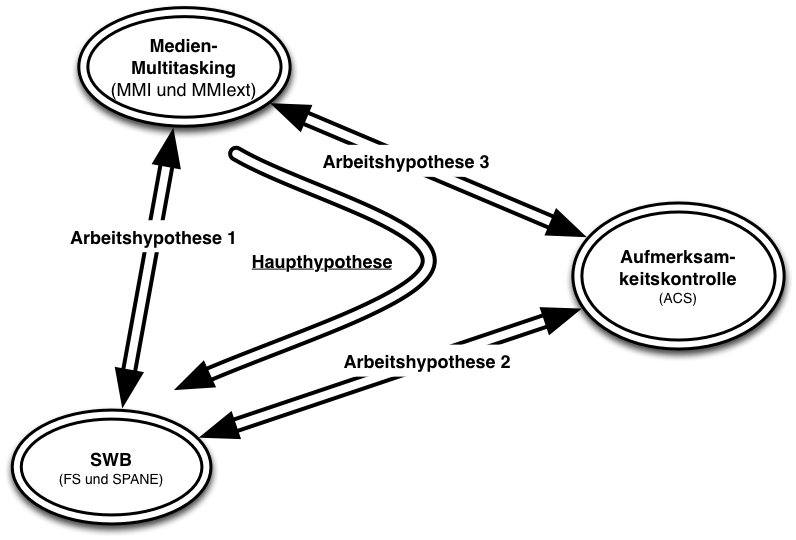
\includegraphics[scale=0.6]{images/grafiken/Hypothesen_Grafisch_v1.png}
     \caption{Zusammenhang Hypothesen}
     \label{pic.einleitung.hypothesen}
\end{figure}






% Methode
%%%%%%%%%%%%%%%%%%%%%%%%%%%%%%%%%%%%%%%%%%%%%%%%%%%%%%%%%%%%%%%%%
%_____________ ___    _____  __      __ 
%\____    /   |   \  /  _  \/  \    /  \  Institute of Applied
%  /     /    ~    \/  /_\  \   \/\/   /  Psychology
% /     /\    Y    /    |    \        /   Zuercher Hochschule 
%/_______ \___|_  /\____|__  /\__/\  /    fuer Angewandte Wissen.
%        \/     \/         \/      \/                           
%%%%%%%%%%%%%%%%%%%%%%%%%%%%%%%%%%%%%%%%%%%%%%%%%%%%%%%%%%%%%%%%%
%
% Project     : Bachelorarbeit
% Title       : Methode
% File        : methode.tex Rev. 00
% Date        : 06.12.2013
% Author      : Till J. Ernst
%
%%%%%%%%%%%%%%%%%%%%%%%%%%%%%%%%%%%%%%%%%%%%%%%%%%%%%%%%%%%%%%%%%
\glsresetall
\chapter{Methode (Vergangenheit)}

% Kapitel Studiendesign
%---------------------
\section{Studiendesign}\label{section.studiendesign}
In der vorliegenden Studie handelt es sich um eine empirische Querschnitts-Studie mit quantitativem Charakter. Die Generierung der Daten für die Beantwortung der Fragestellung erfolgte mittels Internet-Fragebogen. Dazu wurden die für die Hypothesen relevanten Parameter empirisch erhoben und mittels deskriptiver Statistik ausgewertet. Um eine möglichst umfassende Beantwortung der Forschungsfrage zu ermöglichen, wurde eine grösstmögliche Stichprobe von Probanden angestrebt, die täglich Medien nutzen. Bei den befragten Probanden handelte es sich um Studierende, die aktuell ein Studium an einer Universität oder einer Fachhochschule in der Schweiz absolvieren. Der Fragebogen wurde in deutscher Sprache verfasst, weshalb ausschliesslich Schulen der deutschsprachigen Schweiz berücksichtigt wurden.\\
Diese Studie verfolgte das Ziel, mögliche Tendenzen aufzuzeigen. Durch die Befragung einer spezifischen Bevölkerungsgruppe können die Resultate nicht verallgemeinert werden und dienen einer exemplarischen Betrachtung.

%---------------------
\subsection{Hauptzielparameter}\label{subsection.hauptzielparameter}
Die folgenden Hauptzielparameter dienten zur Beantwortung der Fragestellung (siehe \nameref{section.fragestellung}). Einen möglichen Einflusses von Medien-Multitasking auf das subjektive Wohlbefinden wurde mittels bereits existierender Fragebögen erhoben. Diese Fragebögen dienten zur Erfassung der Häufigkeit der Nutzung von einzelnen Medien, der Häufigkeit der simultanen Mediennutzung, der Fähigkeit der simultanen Mediennutzung und des aktuellen subjektiven Wohlbefindens der Probanden. Mittels Erhebung der demographischen Daten wurde das Geschlecht, Alter, Studienform (Teilzeit- oder Vollzeitstudium), Schulform (Universität oder Fachhochschule), berufliche Tätigkeit, Zivilstand und Familienstatus erhoben. Diese Daten dienten zur Aufteilung der Stichprobe in verschiedene Gruppen, um mögliche Einflüsse auf das subjektive Wohlbefinden anhand demographischer Daten zu untersuchen.

%---------------------
\subsection{Durchführung der Untersuchung}
Die Durchführung dieser Arbeit erfolgte im Rahmen einer Bachelorarbeit an der Zürcher Hochschule für angewandte Wissenschaften im Bereich angewandter Psychologie. Die gesamte Projektdauer betrug sechs Monate und wurde im Zeitrahmen des Frühlingssemesters 2014 durchgeführt.

% Kapitel Auswahl der Versuchspersonen
%---------------------
\section{Auswahl der Versuchspersonen}\label{section.auswahlVersuchsp}
Gemäss Fragestellung wurde der Einfluss von Medien-Multitasking auf das subjektive Wohlbefinden von Studierenden untersucht. Dazu wurden Studierende aus der deutschsprachigen Schweiz, die an einer Universität oder Fachhochschule studieren, mittels Fragebogen zu ihrem Medien-Multitasking Verhalten befragt. Die Schulen wurden anhand der von SWITCH \cite{Switch2014} zur Verfügung gestellten Liste der Universitäten und Fachhochschulen der Schweiz ausgewählt (SWITCH ist ein Hochleistungsnetzwerk der Schweiz, welches die Verbindung von Internetnutzer weltweit und für die Vernetzung von Fachhochschulen im Bereich Schweizer Wissenschaft zuständig ist). Prinzipiell wurde versucht alle Studierenden der ausgewählten Schulen zu erreichen, die entweder im Teilzeit- oder Vollzeitmodus studieren. \\
Mit Hilfe der Poweranalyse \cite{Faul2009} wurde für die Stichprobenumfangsplanung die angestrebte  Stichprobengrösse im Vorfeld auf $N = 134$ angesetzt. Diese Grösse wurde mittels der Software G*Power Version 3.1 für Apple Computer für die Beantwortung der ungerichteten Hauptfragestellung mittels Bivariater-Korrelation berechnet. Folgende Werte wurden dazu verwendet: Es wurde von einem gewünschten mittlerer Effekt $r = .3$  \cite{Cohen1988} für den Korrelationskoeffizienten ausgegangen, einem Signifikanzniveau von $\alpha=.05$ und einer Teststärke von $1-\beta=.95$.
%---------------------
\subsection{Rekrutierung}\label{subsection.rekrutierung}
Die Rekrutierung der Studierenden an den Universitäten und Fachhochschulen der deutschen Schweiz erfolgte wenn immer möglich direkt über die Mailverteiler der einzelnen Schulen (Liste der angeschriebenen Schulen siehe Anhang \ref{chap.appendix_schulListe}). Damit für diese Untersuchung eine möglichst grosse Stichprobe generiert werden konnte, wurde wenn immer möglich innerhalb der einzelnen Schulen die einzelnen Departemente separat angeschrieben. Da diese Mailverteiler der Schulen in den meisten Fällen nicht öffentlich zugänglich sind, wurde direkt versucht auf den einzelnen Schulsekretariaten oder Departementsstellen (z.B.: Dekanat) die Umfrage zu platzieren. Dies wurde teilweise mittels telefonischem Kontakt und teilweise per vordefiniertem Mail vorgenommen. Das Mailing, das zu diesem Zweck erstellt wurde, ist in Anhang \ref{chap.appendix_mailing} zu finden. In diesem Schreiben wurden die einzelnen Schulen um Unterstützung gebeten, in dem sie die Umfrage an ihre Studierenden weiter leiteten. Für die Weiterleitung an die Studierenden wurde dem Mailing eine beschreibende Nachricht der Studie mit dem Link zum Fragebogen angehängt. \\
Schulen die eher konservativ gegenüber Umfragebögen anderer Schulen eingestellt sind, lehnen das Weiterleiten der Umfrage an die Studierenden oftmals ab. Für diese Fälle wurde ein Aushang für das schwarze Brett der Schule erstellt, welcher auf Wunsch der entsprechenden Stelle nachgeliefert und von den Studiumsverantwortlichen selbständig angebracht werden konnte (siehe Aushang Anhang \ref{chap.appendix_aushang}). \\
In dieser Untersuchung wurde das Mailing an über 70 Stellen der in Kapitel \ref{section.auswahlVersuchsp} genannten Schulen und deren Departemente versendet.
%---
\subsection{Einschlusskriterien}\label{subsection.einschlusskriterien}
Alle Studierende von Universitäten und Fachhochschulen aus dem deutschsprachigen Raum, die einem Teilzeit- oder einem Vollzeitstudium nachgehen.
%---
\subsection{Ausschlusskriterien}\label{subsection.ausschlusskriterien}
Ausgeschlossen werden Studierende eines Fernstudiums, da hier weitere Bedingungen gegeben sind, die eine Vergleichbarkeit erschwert. Der Fragebogen wird lediglich auf Deutsch zur Verfügung gestellt. Aus diesem Grund wurden nur Personen berücksichtigt, die der deutschen Sprache mächtig sind. 


% Kapitel Erhebungsinstrumente
%---------------------
\section{Erhebungsinstrumente}\label{section.erhebungsinstrumente}
Die Erhebung der vorliegenden Arbeit basiert auf bereits existierenden Fragebögen aus Studien und der Erfassung von soziodemographischen Daten. Diese Fragen wurde in Form einer Onlineumfrage umgesetzt. In den folgenden Kapiteln werden die zur Überprüfung der Hypothesen verwendeten Fragebögen in der Reihenfolge der Durchführung beschrieben. Diese Fragebögen wurden aus dem Englischen übersetzt, deren Übersetzungen sich im Anhang \ref{chap.appendix_mediaUseQuestionnaire} und folgende befinden. \\
\subsection{Soziodemographischen Daten}\label{subsection.soziDaten}
Bei den soziodemographischen Daten wurden folgende Parameter erfasst: Geschlecht, Alter, Studium (Universität oder Fachhochschule), Studienrichtung, Studentenstatus (Vollzeit- oder Teilzeitstudium), Berufsstand (arbeitstätig neben dem Studium), Zivilstand und Familienstatus (Kinder). \\
%---
\subsection{Media Use Questionnaire und Media Multitasking Index}\label{subsection.muq}
Für die Bestimmung des Multitasking-Verhaltens wurde der \textit{Medien Multitasking Index} generiert. Dieser Index wurde mittels Fragebogenerhebung berechnet, der die Häufigkeit der Nutzung von einzelnen Medien und die gleichzeitige Nutzung verschiedener Medien miteinander misst. Der Medien Multitasking Index und der Fragebogen zur Häufigkeit von Mediennutzung basieren auf dem von \citeA{Ophir2009} entwickelten \textit{\gls{labelMMI}} und dem \textit{\gls{labelMUQ}}. Diese Instrumente wurden für diese Arbeit aus dem Englischen ins Deutsche übersetzt (siehe Anhang \ref{chap.appendix_mediaUseQuestionnaire}). Der Fragebogen registriert wie viele Stunden eine Person eine von 12 vordefinierten Medienformen in einer Woche nutzt und wie oft diese Person diese Medienform mit anderen Medienformen simultan verwendet. \\ 
Für dieser Umfrage wurde der \gls{labelMMI} leicht angepasst. Anstelle von ganzen Stunden in einer Woche, wurde die durchschnittliche Anzahl Minuten an einem Tag erfasst. Dies erschien für Medien wie Textnachrichten einfacher abschätzbar zu sein. Für die Berechnung des \gls{labelMMI} mussten anschliessend die erfassten Minuten in Stunden einer Woche hochgerechnet werden. Dies wurde mittels folgender Formel berechnet: \(\frac{n_{i} \times 7_{(Tage)}}{60}\). \(n_{i}\) entspricht der Anzahl Minuten pro Tag, die für die Nutzung eines Mediums verwendet werden.\\
Die für die Mediennutzung erfassten Medien beliefen sich auf 12 Medienformen. Diese waren Druckmedien, Fernsehen, Online Video (wie zum Beispiel Youtube), Musik, Nicht-musikalische Audiomedien (z.B. Hörbücher, Podcast, etc.), Video oder Computer Games, Telefonieren (Mobil- und / oder Festnetz), Instant Messaging (z.B. Skype, Windows Live Messenger, Yahoo Messenger, etc.), SMS (Textnachrichten), Email, Internet-Surfen und Andere Computerbasierte-Tätigkeiten (z.B. Word, Videobearbeitung, programmieren, etc.). \\
Neben der Nutzungsdauer einzelner Medien wurde die gleichzeitige Nutzung verschiedener Medien mittels Medien-Multitasking-Matrix gebildet. Diese bestand im Wesentlichen aus den 12 definierten Medien, die in Hauptmedien (vertikale Spalte) und Nebenmedien (horizontale Zeile) aufgeteilt wurden. Die Aufgabe für die Probanden bestand darin, zu jedem Hauptmedium eine Schätzung abzugeben, wie oft ein weiteres Nebenmedium gleichzeitig zusammen mit dem jeweiligen Hauptmedium verwendet wurde. Die Bewertung innerhalb der Matrize erfolgte mittels definierter Auswahl \textit{meistens}, \textit{etwas}, \textit{wenig} oder \textit{nie}.\\
Mittels der Medien-Nutzungsdauer und der gleichzeitigen Nutzung einzelner Medien wurde der Medien Multitasking Index gebildet. Hierbei ist zu beachten, dass die Textnachrichten in der ursprünglichen Formel gemäss \cite{Ophir2009}  nicht berücksichtigt wurden. Die Autoren gingen davon aus, dass die Abschätzung der Nutzung von Textnachrichten in Stunden nicht exakt vorgenommen werden konnte und liessen sie deshalb weg. Dieses Medium wurde im ursprünglichen Fragebogen als Sekundärmedium belassen. In dieser Studie wurde die Erfassung der Medien-Nutzung in Minuten vorgenommen, weshalb die Textnachrichten als Hauptmedien dazu gezählt wurden. Die angepasste und die ursprüngliche Formel für die Berechnung des Indexes lautete:
%Formel
\begin{equation}\label{formel.mmiext}
    MMI_{ext}=\sum_{i=1}^{12} \frac{m_{i} \times \frac{n_{i} \times 7_{(Tage)}}{60}}{h_{total}}
\end{equation}
%Formel
\begin{equation}\label{formel.mmi}
    MMI=\sum_{i=1}^{11} \frac{m_{i} \times h_{i}}{h_{total}}
\end{equation}
In der ursprünglichen Formel $MMI$ steht \(h_{i}\) für die Anzahl Stunden pro Woche, die für ein Hauptmedium \(i\) verwendet wurde. In der angepassten Formel $MMI_{ext}$ wird die Anzahl Stunden pro Woche aus der Anzahl Minuten pro Tag \(n_i\) auf eine Woche hochgerechnet (\(h_{i}=\frac{n_{i} \times 7}{60}\)). \(h_{total}\) steht für die totale Anzahl Stunden aller Medien, die in einer Woche verwendet werden. \(m_i\) beinhaltet die Summe der Abschätzungen des Probanden bezüglich seiner simultanen Nutzung eines oder mehrerer Nebenmedien. Die Summenbildung ergibt die durchschnittliche Anzahl der Medien, die neben dem Hauptmedium verwendet werden. Für die Berechnung wurde den Abschätzungen der Probanden numerische Werte wie folgt zugewiesen: 1 = \textit{meistens}, .67 = \textit{etwas}, .33 = \textit{wenig} oder 0 = \textit{nie}. Der resultierende Medien Multitasking Index $MMI$ (resp. $MMI_{ext}$) kennzeichnet die durchschnittliche Menge von Medien Multitasking, die während einer typischen Stunde Mediennutzung auftritt. Dieser Index lässt die Unterteilung in Personen zu, die stark Medien-Multitasking betreiben ($HMMs$) und Personen, die schwach Medien-Multitasking betreiben ($LMMs$). Für alle die ein mittleres Medien-Multitasking betreiben, wird die Bezeichnung $NMMs$ verwendet. Für die Unterscheidung dieser beiden Bereiche wurde die Standardabweichung hinzugezogen (eine Standardabweichung oder mehr über dem Mittel für starkes Multitasking und eine Standardabweichung oder weniger unter dem Mittel für schwaches Multitasking): 
%Formel HMMs und LMMs
\begin{equation}\label{formel.hmms}
    HMMs>=M+SD
\end{equation}
\begin{equation}\label{formel.lmms}
    LMMs<=M-SD
\end{equation}

%---  
\subsection{Attentional Control Scale} \label{subsection.acs}
Bei der \textit{Aufmerksamkeitskontroll-Skala} (engl.: \gls{labelACS}) handelt es sich um einen Selbstbeurteilungsfragebogen, der von \citeA{Derryberry2002} für die Messung von individuellen Unterschieden in der Aufmerksamkeitskontrolle entwickelt wurde. Aufmerksamkeit entsteht in miteinander verbundenen Netzwerken im Gehirn, eine davon ist das anteriore Aufmerksamkeitssystem (engl.: anterior attentional system), welches als exekutive Kontrollfunktion über die restlichen Aufmerksamkeitsprozesse waltet \cite{Posner1998}. Aufgrund unterschiedlich vorgeschlagener Funktionen des anterioren Systems, wurde die Aufmerksamkeitskontroll-Skala als Instrument für die Messung allgemeiner Unterschiede in der selbstinitierten Aufmerksamkeitskontrolle entwickelt \cite{Derryberry2001}.\\
Der Fragebogen umfasste 20 Fragen, die Ursprünglich in zwei unterschiedlichen Skalen enthalten waren \cite{Derryberry1988}: Ausrichten der Aufmerksamkeit und Aufmerksamkeitsverschiebung. Unter der Ausrichtung der Aufmerksamkeit verstanden die Forscher die Kapazität, den Aufmerksamkeitsfokus absichtlich in ein gewünschte Richtung zu lenken, ohne sich dabei unabsichtlich von irrelevanten oder störenden Reizen ablenken zu lassen. Unter Aufmerksamkeitsverschiebung verstanden die Forscher die Kapazität, die Aufmerksamkeit absichtlich von einer Richtung in die andere Richtung zu lenken und dabei die Aufmerksamkeit nicht in eine spezifische Richtung zu fokussieren. In den letzten Jahren wurden die zwei Skalen unter dem Sammelbegriff der Aufmerksamkeitskontroll-Skala zusammengefasst, die als Messmittel für die Fähigkeit der Aufmerksamkeitskontrolle diente. Gemäss \citeA{Derryberry2002} ergab die Faktoranalyse des \gls{labelACS} bezogen auf die Fähigkeit einen Zusammenhang aus wechselseitigen Subfaktoren wie (a) sich auf etwas zu fokussieren, (b) zwischen verschiedenen Aufgaben hin und her zu wechseln und (c) eine flexible Gedankenkontrolle \cite{Derryberry2002}. \\
Die \gls{labelACS} wurde für diese Untersuchung aus dem Englischen übersetzt (siehe Anhang \ref{chap.appendix_attentionalControlScale}). Die Skala des ACS bestand aus 20 Fragen, die mittels vierstufiger Likert-Skala beantwortet werden konnten (1 = fast nie; 2 = manchmal; 3 = oft; 4 = immer). Je höher die Antwortzahl ausgefallen ist, desto höher war die Aufmerksamkeitskontrolle des Probanden (Max. 80 Punkte, Min. 20 Punkte). Hierbei ist zu beachten, dass 11 der 20 Fragen für die Bewertung invertiert werden mussten. Dies waren die Fragen 1 bis 3, 6 bis 8, 11, 12, 15, 16, 18 und 20.

%---
\subsection{Flourishing Scale und Scale of Positive and Negative Experience} \label{subsection.flourishingScale}
Die von \citeA{Diener:2010} entwickelte Skalen \textit{\gls{labelFS}} und \textit{\gls{labelSPANE}} sind Fragebögen für die Erfassung des psychologischen und sozialen Wohlbefindens. Mit diesen Skalen wurde das psychosoziale Aufblühen (aus dem Englischen von flourishing), basierend auf dem psychologischen und sozialem Wohlbefinden, und dem positiven und negativen Befinden, erfasst. \\
Die \gls{labelFS}-Skala wurde auf dem Hintergrund von sozialen Beziehungen entwickelt. Aus dem englischen übersetzt steht \textit{flourishing} im Zusammenhang mit Glück für menschliches Aufblühen, wachsen, entfalten und gutem Gedeihen \cite{Esch2014}. In dieser Arbeit wird vom menschlichen Aufblühen gesprochen, wenn auf diese Skala referenziert wird. Der Fragebogen erfasste menschliches Aufblühen in relevanten Bereichen wie Lebensinhalt, Beziehungen, Selbstwertgefühl, Gefühl der Kompetenz und Optimismus \cite{Silva2013}. Dieser Bereich von positivem Funktionieren scheint einen signifikanten Einfluss auf das persönliche Wohlbefinden zu haben \cite<e.g.,>{Ryan2000, Ryff1989}.
Die Skala umfasste acht Items aus wichtigen Bereichen des menschlichen Funktionierens, wie positive Beziehungen, Gefühle der Kompetenz und Führen eines zielgerichteten und sinnvollen Lebens \cite{Diener:2010}.\\ 
Die aus dem Englisch stammenden Fragen wurden für diese Arbeit ins Deutsche übersetzt (siehe dazu Anhang \ref{chap.appendix_fs}). Jedes Item konnte auf einer Skala von 1 - 7 beantwortet werden. Von 1 = trifft überhaupt nicht zu bis zu 7 = triff voll und ganz zu. Alle Fragen wurden in einer positiven Richtung formuliert. Die Skala verfügte über einen einzigen Ergebniswert für das psychologische Wohlbefinden. Die Summe der Punkte konnte zwischen 8 (trifft überhaupt nicht zu) und 56 (trifft voll und ganz zu) liegen. Hohe Werte deuteten darauf hin, dass sich die befragte Person in einem positiven Licht sieht, bezogen auf ihr Funktionieren und über psychologische Ressourcen und Stärken verfügte. Die Skala zeigte jedoch keine einzelnen Aspekte des Wohlbefindens auf. Vielmehr erstellte sie eine Übersicht aus positivem Funktionieren aus Bereichen des Lebens, die weithin als wichtig angeschauten werden. 
\par
Die Skala für das Erfassung von positiven und negativen Erfahrungen (\gls{labelSPANE}) beinhaltete einen zwölfteiligen Fragebogen, der aus je sechs Items für die Erfassung von positiven und sechs Items für die Erfassung von negativen Empfindungen bestand \cite{Diener:2010}. Mittels dieser 12 Fragen wurde eine weite Bandbreite von negativen und positiven Erleben und Gefühlen abgeschätzt, die mittels Erfassung aller erlebten Gefühlen der vergangenen vier Wochen hergeleitet wurde. Für die Skalen der positiven und der negativen Empfindungen waren drei Fragen genereller Natur (z.B.: positiv, negativ) und drei Fragen spezifischer Natur (z.B.: froh, traurig). Aufgrund der Erfassung von generellen positiven und negativen Gefühlen, erfasste der Fragebogen die gesamte Bandbreite von positiven und negativen Erlebnissen, inklusive spezifischer Gefühle, die unter Umständen in verschiedenen Kulturen unterschiedlich lauten. Dadurch wird angenommen, dass der Fragebogen kulturunabhängig funktionierte \cite{Silva2013}. Des Weiteren erfasste dieser Fragebogen nicht nur die erfreulichen und weniger erfreulichen Emotionen, sondern gab auch Zustände wie Interessen, Flow, positives Engagement und physikalischer Freude wieder.\\
Jede Frage des \gls{labelSPANE}-Fragebogens wurde auf einer fünfstufigen Likert Skala von 1 bis 5, von 1 = sehr selten oder nie, bis 5 = sehr oft oder immer, beantwortet. Die positive und die negative Skala wurden aufgrund der teilweise unabhängigen Typen der Empfindungen separat ausgewertet. Die einzelnen Fragebogenitems wurden aus dem Englischen ins Deutsche übersetzt und sind im Anhang \ref{chap.appendix_spane} aufgeführt. Die Summe der positiven Resultate ($SPANE-P$) sowie der negativen Resultate ($SPANE-N$) konnten zwischen einem Bereich von 6 und 30 liegen. Die Skala $SPANE-P$ beinhaltete die positiven Gefühle positiv, gut, angenehm, glücklich, froh und zufrieden. Die Skala $SPANE-N$ beinhaltete die negativen Gefühle negativ, schlecht, unangenehm, traurig, ängstlich und wütend. Diese beiden Skalen konnten miteinander kombiniert werden, indem die Resultate der negativen Gefühl-Skala von der positiven Gefühl-Skala abgezogen wurde. Die Summe dieser neuen Skala ($SPANE-B$) konnte zwischen -24 (am unglücklichsten) und 24 (höchste Affektstabilität) liegen. Probanden mit einem sehr hohen Ergebnis von 24 gaben an, dass sie selten oder nie negative Gefühle erleben und sehr oft oder immer positive Gefühle verspüren.


% Kapitel Datenerhebung
%---------------------
\section{Datenerhebung}\label{section.datenerhebung}
Die Datenerhebung erfolgte mittels elektronischer Online-Befragung. Diese Befragung wurde mit Hilfe der von der ZHAW zur Verfügung gestellten Umfragesoftware EFS Survey von QuestBack Unipark \cite{QuestBack2014} erstellt. Der Fragebogen wurde anhand der zur Verfügung gestellten Dokumentation erstellt. Die Befragung erfolgte zu Beginn des Frühlingssemesters 2014 und wurde für den Zeitraum von vier Wochen aktiv geschaltet. Der Zugang zur Befragung erfolgte über die von der QuestBack Unipark bereitgestellte Internetadresse, welcher zum Zeitpunkt der Befragung wie folgt lautete: \url{http://www.unipark.de/uc/multitasking_and_swb/}.\\
Die Umsetzung der Erhebungsinstrumente erfolgte anhand von der Software vorgegebenen Fragemasken. Ein Auszug des Fragebogens in Papierform ist im \nameref{chap.appendix_fragebogen} zu finden. Dabei ist zu beachten, dass die Umsetzung in Papierform von der originalen Umfrage in digitaler Form abweichen kann. Der Fragebogen beinhaltete zu Beginn eine kurze Einführung mit der Anonymitätserklärung der Datenerhebnung und dem Hinweis auf den Wettbewerb. Danach folgten die einzelnen Erhebungsinstrumente, beginnend mit der Erfassung der demographischen Daten, gefolgt vom Mediennutzungs-Fragebogen, dem Aufmerksamkeitskontroll-Skala und dem Fragebogen zum Wohlbefinden. Am Ende der Befragung konnten sich die Teilnehmer für die Teilnahme an einem Wettbewerb für Gutscheine im Athleticum Sportmarket \cite{Athleticum2014} eintragen. Neben dem Wettbewerb konnten sich die Teilnehmer für die Ergebnisse der Studie eintragen, die am Ende dieser Arbeit versendet werden. \\
Der Fragebogen wurde mittels Pretest auf seine Funktionalität hin überprüft und erfolgte in zwei Schritten. Einerseits erlaubte die von QuestBack Unipark zur Verfügung gestellte Software eine elektronische Testung des Fragebogens. Dabei ging es um die Wählbarkeit der Frageoptionen und der Erreichbarkeit aller aufgestellter Fragen. In einem weiteren Schritt wurden 15 willkürlich ausgewählte Testpersonen aus dem Bekanntenkreis des Autors als Testpersonen rekrutiert, mit der Anweisung, den Fragebogen auszufüllen. Damit sollte sichergestellt werden, dass die Fragen und deren Anweisung verständlich formuliert wurden und die Beantwortung der Fragen möglich war. Vor der Aktivschaltung des Fragebogens wurden alle bis dahin erfassten Daten der Tester gelöscht und die gesamte Umfrage frisch initialisiert. 


% Kapitel Datenaufbereitung
%---------------------
\section{Datenaufbereitung}\label{section.datenaufbereitung}
Die erhobenen Daten wurden mittels SPSS Version 20 für Mac OS X aufbereitet. Die Stichprobendaten wurden direkt aus dem Fragebogen Onlinewerkzeug QuestBack Unipark \cite{QuestBack2014} mittels Datenexport für SPSS importiert. Allfällige Fehlerquellen wurden bei der Datenbereinigung korrigiert. Dies wurde durch die Umfragesoftware erleichtert, indem nur abgeschlossene Datensätze exportiert wurden und eine erste Werteprüfung bei der Eingabe erfolgte (z.B.: es wurden nur Zahlen bei der Eingabe des Alters zugelassen). Fehlende Werte wurden bereits von der Umfragesoftware gesetzt und konnten innerhalb von SPSS mit einem Wertelabel versehen werden. Für die Berechnung des Mulitmedia Indexes $MMI$ \cite{Ophir2009}, die Aufmerksamkeitskontroll-Skala  $ACS$ \cite{Posner1998}, die Skala des menschlichen Aufblühens $FS$ \cite{Diener:2010} und die Skala für das Erfassung von positiven und negativen Erfahrungen $SPANE-P$ und $SPANE-N$ \cite{Diener:2010} wurden zusätzliche Variablen in SPSS erstellt und anhand der von Umfrage übernommenen Werten berechnet. 

% Kapitel Statistische Verfahren
%---------------------
\section{Statistische Verfahren}\label{section.statistischeVerfahren}
Für die Beantwortung der Fragestellung erfolgte nach der Datenerfassung und der Datenaufbereitung die Datenauswertung. In einem ersten Schritt wurde eine deskriptive, univariate Analyse der Stichprobendaten durchgeführt, um mögliche Fehler bei der Datenerfassung und/oder Ausreisser im Datensatz zu entdecken. Dies erfolgte mittels Häufigkeitsverteilung, um die verschiedenen Merkmalsausprägungen einer Variablen im Datensatz zu beschreiben und mittels Verteilungsparameter, die die Verteilung der Merkmalsausprägung charakterisieren (Lage- und Streuungsparameter). Des weiteren wurde die Schiefe der Häufigkeitsverteilung gegenüber der Normalverteilung überprüft. Die Prüfung der Normalverteilung wurde mittels Sichtvergleich vorgenommen. Dazu wurde eine Graphik der Häufigkeitsverteilung der Stichprobendaten mit einem Bild einer Normalverteilung verglichen. Diese optische Prüfung erfolgte mit Hilfe von SPSS und der Darstellung eines Histogramms, das mit einer Häufigkeitsauszählung und der Darstellung der Normalverteilungskurve ausgegeben wurde. Ebenfalls mit SPSS wurde zusätzlich ein Q-Q-Diagram (Quantile-Quantile-Plot) erstellt, welches die Stichprobendaten mit einer Gerade vergleicht, die eine Normalverteilung repräsentiert. Anschliessend an die deskriptive Analyse wurde in einem weiteren Schritt die statistischen Zusammenhänge der Stichprobendaten für die Haupthypothese und die Arbeitshypothesen berechnet. \par 
\textbf{Haupthypothese:} Ziel dieser Hypothese war es die Häufigkeit von Medien-Multitasking (MUQ) und die kognitive Fähigkeit (Aufmerksamkeitskontrolle) als treibenden Faktor für den Einfluss von Medien-Multitasking auf das subjektive Wohlbefinden zu benennen. Für diese Beantwortung wurde einerseits der Zusammenhang zwischen Medien-Multitasking und Aufmerksamkeitskontrolle und der Zusammenhang zwischen Aufmerksamkeitskontrolle und subjektiven Wohlbefinden mittels Produkt-Moment-Korrelationskoeffizienten (Pearson-Korrelations-Koeffizienten) berechnet (siehe Arbeitshypothesen weiter unten). Anschliessend wurde mittels Partialkorrelation der Scheinzusammenhang der Variable Aufmerksamkeitskontrolle berechnet. Das Signifikanzniveau der Analyse liegt bei $p=.05$. Es wurden die Werte gemäss \cite{Cohen1988} übernommen, um Aussagen über die Stärke des Effekts zu machen ($r=.10$ -- kleine Effektstärke; $r=.30$ -- mittlerer Effektstärke; $r=.50$ -- grosse Effektstärke). Zudem wurden heterogene Untergruppen weitgehend aufgeteilt und jeweils einen gesonderten Korrelationskoeffizienten gebildet \cite{Renkewitz2008}. Dies wurde angewendet, um verdeckte Korrelationen zwischen heterogenen Untergruppen aufzudecken \cite{Ebermann2014}.

\textbf{Arbeitshypothesen:} Ziel der Arbeitshypothesen war es den Zusammenhang zwischen Medien-Multitasking und dem subjektiven Wohlbefinden, den Zusammenhang zwischen der kognitiven Fähigkeit und dem subjektiven Wohlbefinden und den Zusammenhang zwischen der kognitiven Fähigkeit und der Häufigkeit von Medien-Multitasking zu belegen. Dies wurde mittels Produkt-Moment-Korrelationskoeffizienten (Pearson-Korrelations-Koeffizienten) berechnet. Das Signifikanzniveau der Analyse liegt bei $p=.05$. Wiederum wurden heterogene Untergruppen aufgeteilt, um verdeckte Korrelationen aufzudecken \cite{Ebermann2014}. \par









% Ergebnisse
%%%%%%%%%%%%%%%%%%%%%%%%%%%%%%%%%%%%%%%%%%%%%%%%%%%%%%%%%%%%%%%%%
%_____________ ___    _____  __      __ 
%\____    /   |   \  /  _  \/  \    /  \  Institute of Applied
%  /     /    ~    \/  /_\  \   \/\/   /  Psychology
% /     /\    Y    /    |    \        /   Zuercher Hochschule 
%/_______ \___|_  /\____|__  /\__/\  /    fuer Angewandte Wissen.
%        \/     \/         \/      \/                           
%%%%%%%%%%%%%%%%%%%%%%%%%%%%%%%%%%%%%%%%%%%%%%%%%%%%%%%%%%%%%%%%%
%
% Project     : Bachelorarbeit
% Title       : Ergebnisse
% File        : ergebnisse.tex Rev. 00
% Date        : 06.12.2013
% Author      : Till J. Ernst
%
%%%%%%%%%%%%%%%%%%%%%%%%%%%%%%%%%%%%%%%%%%%%%%%%%%%%%%%%%%%%%%%%%
\glsresetall
%####################################################
% Kapitel Ergebnisse
%####################################################
\chapter{Ergebnisse (Vergangenheit)}
TBD: Zusammenfassung der folgenden Kapitel.\\
Verweis auf den Anhang mit der Mittelwertstabelle.

%####################################################
% Kapitel Deskriptive Analyse der Stichprobendaten
%####################################################
\section{Deskriptive Analyse der Stichprobendaten}
\label{label.stichprobe}
Die Stichprobe belief sich nach Beendigung der Umfrage auf 1376 Personen, die den Fragebogen komplett abgeschlossen haben ($N = 1367$). Insgesamt haben 2181 Personen zumindest den Link für die Onlinebefragung angeklickt. Davon wiederum haben 1943 Personen die Umfrage begonnen, was einer Ausschöpfungsquote von 89.1\% entspricht. 29.6\% derjenigen, die den Fragebogen zumindest angefangen haben, haben die Umfrage nicht bis zum Schluss durchgeführt. Wie bereits zu Beginn erwähnt, haben 1376 Personen die Befragung abgeschlossen, was einer Beendigungsquote von 62.7\% entspricht.\\
Die mittlere Bearbeitungszeit der Umfrage belief sich auf 15 Minuten und 44 Sekunden. Durchschnittlich haben den Fragebogen 81 Personen pro Tag ausgefüllt. Auf zwei Seiten des Fragebogens wurden die meisten Abbrüche verzeichnet. Bei der einen Seite handelte es sich um die Startseite, die als Einstiegsseite mit den Erläuterungen zur Umfrage und zum Wettbewerb diente, und bei der zweiten Seite handelte es sich um die Befragung zum Medien-Multitasking-Verhalten. Diese beiden erwähnten Seiten können im Anhang \ref{chap.appendix_fragebogen} unter Sektion \nameref{anhangSesction.Startseite} und \nameref{anhangSection.muq} gefunden werden.\\
Im folgenden werden auf die einzelnen Variablen der Stichprobendaten genauer eingegangen. Dazu dienen einzelne Häufigkeitstabellen dem besseren Verständnis. Aus Gründen der Übersichtlichkeit wurden einzelne Tabellen in den Anhang \ref{anhang.hauefigkeitstabelle} verschoben.

% UnterKapitel Demographische Daten
%####################################################
\subsection{Demographische Daten}
Die Studienpopulation belief sich auf 1367 Personen ($N = 1367$), davon waren 960 Personen weiblich (70.2\%), 404 Personen männlich (29.6\%) und 3 Personen, die keine Angabe (.2\%) zu ihrem Geschlecht gemacht haben. Das durchschnittliche Alter betrug zur Zeit der Befragung 25.4 Jahre ($Median=24$; $SD = 6.5$) wobei die jüngste Person 15 Jahre und die älteste Person 67 Jahre alt war. Wie aus Tabelle \ref{table.sozidemoAlter10er} zu entnehmen ist, waren 58.5\% der Befragten zwischen 15 und 24 Jahre alt. 33\% waren zwischen 25 und 34 Jahre alt. Die restlichen waren 35 Jahre und älter (eine detailliertere Aufteilung des Alters ist im Anhang \ref{anhang.hauefigkeitstabelle} in Tabelle \ref{table.sozidemoAlter5} zu finden).\\ 
%Tabelle Altergruppen
\begin{table}[ht]
    \centering 
    \caption{Häufigkeit der Altersgruppen in 10er Schritten, demographische Charakteristik}
    \begin{tabular}[t]{|L{20mm} r|R{20mm}|R{20mm}|R{20mm}|R{20mm}|} 
        \hline
        \multicolumn{6}{|c|}{\textbf{Altersgruppen}}\\        
        \multicolumn{2}{|c}{} & \multicolumn{1}{c|}{Häufigkeit} & \multicolumn{1}{c|}{Prozent} & \multicolumn{1}{c|}{Gültige} & \multicolumn{1}{c|}{Kumulierte}\\
        \multicolumn{2}{|c}{} & \multicolumn{1}{c|}{(N)} & \multicolumn{1}{c|}{(\%)} & \multicolumn{1}{c|}{Prozente} & \multicolumn{1}{c|}{Prozente} \\
        \hline       
        Gültig & 15 - 24 & 799 & 58.4 & 58.5 & 58.5\\
        & 25 - 34 & 457 & 33.4 & 33.5 & 92.0\\
        & 35 - 44 & 64 & 4.7 & 4.7 & 96.7\\
        & 45 - 54 & 41 & 3.0 & 3.0 & 99.7\\
        & > 54 & 4 & .3 & .3 & 100.0\\
        & Gesamt & 1365 & 99.9 & 100 & \\
        Fehlend & System & 2 & .1 & &\\
        Gesamt & & 1367 & 100.0 & &\\
        \hline
    \end{tabular}
    \label{table.sozidemoAlter10er}
\end{table}
Insgesamt studierten 374 Personen der Stichprobe an einer Universität (27.4\%) und 993 an einer Fachhochschule (72.6\%). Der Studentenstatus belief sich auf 1084 Vollzeitstudierende (79.3\%) und 282 Teilzeitstudierende (20.6\%). \\
766 Studierende waren zur Zeit der Befragung berufstätig (56\%) und 601 gingen neben dem Studium keiner genannten Arbeit nach (44\%). Im Durchschnitt arbeiteten diejenigen, die einer Arbeit nachgehen 15 Stunden pro Woche ($Min = .5$ Stunden, $Max = 80$ Stunden pro Woche).\\
1244 der Befragten waren zum Zeitpunkt der Befragung ledig (91\%) und 1286 gaben an, keine eigenen Kinder zu besitzen (94.1\%).

% UnterKapitel Media Multitasking Index
%####################################################
\subsection{Medien Multitasking Index -- MMI}
Der Medien Multitasking Index ($MMI_{ext}$ und $MMI$) kennzeichnet die durchschnittliche Menge von Medien Multitasking, die während einer typischen Stunde Mediennutzung auftritt (siehe dazu auch Kapitel \ref{subsection.muq} - \nameref{subsection.muq}). Wie aus Tabelle \ref{table.deskrptMedien} zu entnehmen ist, belief sich der Mittelwert für $MMI_{ext}$ auf 1,35 ($SD =  1.00$) und für $MMI$ auf $M = 1.29$ ($SD = .97$). Dieser Index lässt die Unterteilung in Personen zu, die schwach Medien-Multitasking ($LMMs$) betreiben und solche, die stark Medien-Multitasking ($HMMs$) betreiben.\\
% Tabelle MMI
\begin{table}[ht] 
    \centering
    \caption{Häufigkeit und Verteilung des Medien-Multitasking-Index}
    \begin{tabular}[t]{|R{40mm} r|r|r|} 
        \hline
        \multicolumn{4}{|c|}{\textbf{Multimedia-Multitasking-Index}}\\ 
        \hline       
        \multicolumn{2}{|c}{} & \multicolumn{1}{c|}{$MMI_{ext}$} & \multicolumn{1}{|c|}{$MMI$}\\
        \multicolumn{2}{|c}{} & \multicolumn{1}{c|}{(Ergebnis mit SMS)} & \multicolumn{1}{|c|}{(Ergebnis ohne SMS)}\\
        \hline
        Gesamtwert (N) & Gültig & 1359 & 1359\\
        & Fehlend & 8 & 8\\
        Mittelwert & $M$ & 1.35 & 1.29\\
        Median & $med$ & 1.16 & 1.10\\
        Standardabweichung & $SD$ & 1.00 & .97\\
        Minimum & $Min$ & .00 & .00\\
        Maximum & $Max$ & 6.48 & 6.38\\
        Starke MMT & $HMMs$ & 2.35 & 2.26\\
        Schwache MMT & $LMMs$ & .35 & .32\\
        \hline
    \end{tabular}
    \label{table.deskrptMedien}
\end{table}
Der Wert für die Unterteilung in starke Medien-Multiasking Nutzer lag beim $MMI_{ext}$ für $HMMs >= 2.35$ ($M + SD$ resp. 1.35 + 1.00) und für schwache Multitasker bei $LMMs <= .35$ ($M - SD$ resp. 1.35 - 1.00). \\
Analog dazu wurden die Werte für die Variable $MMI$ berechnet: $HMMs >= 2.26$ und $LMMs <= .32$. \\

% Table HMM und LMM Häufigkeiten
\begin{table}[ht] 
    \centering
    \caption{Häufigkeit der Mediennutzung}
    \begin{tabular}[t]{|L{25mm} r|R{18mm}|R{18mm}|R{18mm}|R{18mm}|} 
        \hline
        \multicolumn{6}{|c|}{\textbf{Mediennutzung}}\\ 
        \hline       
        \multicolumn{2}{|c}{} & \multicolumn{2}{c|}{$MMI_{ext}$} & \multicolumn{2}{c|}{$MMI$}\\
        \multicolumn{2}{|c}{} & \multicolumn{1}{c|}{Häufigkeit} & \multicolumn{1}{c|}{Prozent}&\multicolumn{1}{c|}{Häufigkeit} & \multicolumn{1}{c|}{Prozent}\\
        \hline
        Gültig & LMMs & 188 & 13,8 & 181 & 13,2\\
        & HMMs & 202 & 14,8 & 207 & 15,1\\
        & NMMs & 969 & 70,9 & 971 & 71,0\\
        &Gesamt & 1359 & 99,4 & 1359 & 99,4\\
        Fehlend & & 8 & ,6 & 8 & ,6\\
        Gesamt & & 1367 & 100 & 1367 & 100\\
        \hline
    \end{tabular}
    \label{table.deskrptMeediennutzung}
\end{table}

Bezogen auf die Mediennutzung (siehe Tabelle \ref{table.deskrptMeediennutzung}) ergab sich zum Zeitpunkt der Befragung für Variable $MMI_{ext}$ eine Häufigkeitsverteilung von $LMMs = 13.8\% (188)$ schwache Medien-Multitasker und $HMMs = 14.8\% (202)$ starke Medien-Multitasker. 70.9\% (969) Personen befanden sich zwischen der Obergrenze $HMMs$ und der Untergrenze $LMMs$. \\
Bezogen auf die Variable $MMI$ waren es $LMMs = 13.2\% (181)$ schwache und $HMMs = 15.1\% (207)$ starke Medien-Multitasker. 71\% (971) Personen befanden sich zwischen $HMMs$ und $LMMs$. 

% UnterKapitel Aufmerksamkeitskontroll-Skala
%####################################################
\subsection{Aufmerksamkeitskontroll-Skala -- ACS}
Die Aufmerksamkeitskontroll-Skala dient zur Erfassung der allgemeinen Unterschiede der Probanden in der selbstinitierten Aufmerksamkeitskontrolle (siehe dazu Kapitel \ref{subsection.acs} - \nameref{subsection.acs}). \\ Für diese Variable füllten alle Probanden ($N=1367$) die Fragen zur Aufmerskamkeitskontrolle korrekt aus. Dabei entstand ein Mittelwert von $M = 53.43$, mit einer Standardabweichung von $SD = 6.82$. Das Minimum belief sich auf einen Wert von $Min = 34$, das Maximum auf $Max = 75$ (mögliches Minimum = 20 und mögliches Maximum = 80). Eine detaillierte Tabelle dieser Werte ist im Anhang \ref{anhang.hauefigkeitstabelle} zu finden.

% UnterKapitel Skala für menschliches Aufblühen
%####################################################
\subsection{Skala für menschliches Aufblühen -- FS und Skala der positiven und Negativen Erfahrungen -- SPANE}
In diesem Teil werden die Variablen, die für die Erfassung des subjektiven Wohlbefindens verwendet werden, deskriptiv beschrieben (siehe dazu Kapitel \ref{subsection.flourishingScale} - \nameref{subsection.flourishingScale}).\\
In Tabelle \ref{table.deskrptFsSpane} steht die Variable FS für das menschliche Aufblühen und weist einen Gesamtwert von $N = 1364$ Personen auf (3 fehlende Werte). Der Mittelwert beträgt $M = 46.44$, mit einer Standardabweichung von $SD = 5.19$. In diesem Sample wurde ein $Min = 17$ und ein $Max = 56$ gemessen (mögliches Minimum = 8 und mögliches Maximum = 56).\\
Die Variablen für das Erfassen der positiven ($SPANE-P$) und negativen ($SPANE-N$) Erfahrungen konnte in einer weitere Variable $SPANE-B$ kombiniert werden. Gemäss Tabelle \ref{table.deskrptFsSpane} wurde diese Skala von $N = 1361$ Personen beantwortet (6 Personen wiesen keine gültigen Werte auf). Die Variabel $SPANE-P$ wies einen Mittelwert von $M = 23.16$ mit einer Standardabweichung von $SD = 3.52$ auf. Der gesamte mögliche Bereich von Minimum 6 bis Maximum 30 wurde ausgeschöpft. Die Variabel $SPANE-N$ wies einen Mittelwert von $M=14.22$ und einer Standardabweichung von $SD=4.02$ auf. Der Bereich ging von einem $Min = 6$ bis zu einem $Max = 29$ (mögliches Minimum = 6, mögliches Maximum = 30). Die zusammengefasste Variabel $SPANE-B$ wies einen Mittelwert von $M = 8.94$ und eine Standardabweichung von $SD = 6.69$ auf. Der Bereich dieser Variabel reichte von einem $Min = -18$, zu einem $Max = 24$ (mögliches Minimum = -24 und mögliches Maximum = 24).
% Tabelle FS und SPANE
\begin{table}[ht] 
    \centering
    \caption{Häufigkeit und Verteilung der Skalen für menschliches Aufblühen und der positiven und Negativen Erfahrungen}
    \begin{tabular}[t]{|R{40mm} r|R{15mm}|R{15mm}|R{15mm}|R{15mm}|} 
        \hline
        \multicolumn{6}{|c|}{\textbf{Flourishing Scale und SPANE}}\\ 
        \hline       
        \multicolumn{2}{|c}{} & \multicolumn{1}{c|}{$FS$} & \multicolumn{3}{c|}{$SPANE$}\\
        \multicolumn{3}{|c|}{} & \multicolumn{1}{c|}{$P$} &  \multicolumn{1}{c|}{$N$} & \multicolumn{1}{c|}{$B$}\\
        \hline
        Gesamtwert (N) & Gültig & 1364 & 1361 & 1361 & 1361\\
        & Fehlend & 3 & 6 & 6 & 6 \\
        Mittelwert & $M$ & 46.44 & 23.16 & 14.22 & 8.94\\
        Median & $med$ & 47& 24 & 14 & 10 \\
        Standardabweichung & $SD$ & 5.19 & 3.53 & 4.02 & 6,69\\
        Minimum & $Min$ & 17& 6 & 6 & -18 \\
        Maximum & $Max$ & 56& 30 & 29 & 24 \\
        \hline
    \end{tabular}
    \label{table.deskrptFsSpane}
\end{table}
%####################################################
% Kapitel Normalverteilung
%####################################################
\section{Normalverteilung der Variablen}
Für die folgenden Prüfung der Haupthypothese und der Arbeitshypothesen wurden die Variablen für das Medien-Multitasking Verhalten, die Aufmerksamkeitskontrolle und das subjektive Wohlbefinden auf ihre Normalverteilung hin geprüft. Dazu wurden die Variablen $MMI$, $MMI_{ext}$, $ACS$, $FS$ und $SPANE$ mit Hilfe von SPSS und der Darstellung eines Histograms und eines Q-Q-Diagrams (Quantile-Quantile-Plot) optisch überprüft und als normalverteilt befunden.
%####################################################
% Kapitel Arbeitshypothese 1
%####################################################
\section{Arbeitshypothese 1: Auswirkung von Medien-""Multitasking auf das SWB}\label{label.ergebnisse.arbeitshypothese1}
Die Arbeitshypothese 1 lautete: Zwischen der Häufigkeit, wie Medien-Multitasking angewendet wird und dem subjektiven Wohlbefinden, besteht ein negativer Zusammenhang. Je mehr Media-Multitasking angewendet wird, desto negativer wirkt sich dies auf das subjektive Wohlbefinden aus. Zur Überprüfung der Hypothese wurde diese wie folgt operationalisiert:\par
Nullhypothese $H_{0}$:\\
Es gibt keinen Zusammenhang zwischen dem Medien-Multitasking Verhalten und dem subjektiven Wohlbefinden. Der Korrelationskoeffizient unterscheidet sich nicht signifikant von Null ($r=0$). Das heisst, zwischen der Variable Medien Multitasking Index $MMI$ und der Variable $FS$ oder der Variable $SPANE$  besteht kein signifikanter Zusammenhang ($p \geq .05$ (5\%)).
\par
Alternativhypothese $H_{1}$:\\
Es gibt einen ungerichteten Zusammenhang zwischen dem Medien-Multitasking Verhalten und dem subjektiven Wohlbefinden. Der Korrelationskoeffizient unterschiedet sich signifikant von Null ($r \neq 0$). Das heisst, zwischen der Variable Medien Multitasking Index $MMI$ und der Variable $FS$ oder der Variable $SPANE$ besteht ein signifikanter Zusammenhang ($p < .05$ (5\%)).
\subsection{Linearer Zusammenhang}
Für die Annahme oder die Verwerfung der Hypothesen wurde zwischen der Variablen $MMI_{ext}$ (resp. $MMI$) und den für das subjektive Wohlbefinden relevanten Variablen $FS$ und $SPANE$ (aufgeteilt in die Unterskalen $P$, $N$ und $B$) der Pearson-Korrelations-Koeffizient gebildet. Die beiden Variablen $MMI_{ext}$ und $MMI$ wurden aus Gründen der Darstellung zusammengefasst (siehe Tabelle \ref{table.korrelationMmi}). \\
Für die Variable $MMI_{ext}$ und $SPANE-N$ konnte ein kleiner Zusammenhang von $r=.114$, bei einer Signifikanz von $p=.01$, bei einer Stichprobengrösse von $N=1353$ festgestellt werden. Für diesen Zusammenhang kann die Nullhypothese verworfen und die Alternativhypothese angenommen werden. Für die restlichen Variablen, die das subjektive Wohlbefinden repräsentieren, konnte mit der Variable $MMI_{ext}$ kein signifikanter Zusammenhang nachgewiesen werden. Hierbei muss die Nullhypothese angenommen und die Alternativhypothese verworfen werden.\\
Für die Variable $MMI$ ergab sich ein ähnliches Bild. Es konnte ein kleiner Zusammenhang von $r=.107$ ($p=.01$) bei einer Stichprobe von $N=1353$ zwischen $MMI$ und $SPANE-N$ gefunden werden. Auch hier kann somit die Nullhypothese verworfen und die Alternativhypothese angenommen werden. Für die restlichen Kombinationen konnte kein Zusammenhang festgestellt werden und somit musste die Nullhypothese angenommen werden.
% Verdeckte Zusammenhänge
\subsection{Verdeckte Korrelationen}
Um verdeckte Korrelationen zwischen Medien-Multitasking und dem subjektiven Wohlbefinden in dieser Stichprobe zu ermitteln, wurden die Daten anhand des Geschlechts, des Alters und anhand der Mediennutzung aufgeteilt. \par
% --- Aufteilung nach Geschlecht
\textbf{Aufteilung anhand der Variable Geschlecht:} \\
Wie aus Tabelle \ref{table.ergebnis.geschlecht} hervorgeht, weisen die weiblichen Teilnehmer ($N=951$) einen leichten Zusammenhang zwischen der Variable $MMI_{ext}$ und $SPANE-N$ von $r=.126$ ($p=.01$) und zwischen  $MMI_{ext}$ und $SPANE-B$ von $r=-.101$ ($p=.01$) auf. Ein ähnliches Bild ergibt sich für die Variable $MMI$: $r=.119$ ($p=.01$) für den Zusammenhang mit $SPANE-N$ und $r=-.101$ ($p=.01$) für den Zusammenhang mit $SPANE-B$.\\
Bei den männlichen Teilnehmer ($N=401$) konnte keine Zusammenhang zwischen Medien-Multitasking und dem subjektiven Wohlbefinden gefunden werden (weder bei $MMI_{ext}$ noch bei $MMI$).\par
% --- Aufteilung nach Alter
\textbf{Aufteilung anhand der Variable Alter (Mediansplit):} \\
Wird die Stichprobe anhand dem Median des Alters unterteilt ($Median=24$ siehe \ref{label.stichprobe}) so ergibt sich eine leichte Korrelation von $r=.134$ ($p=.01$) zwischen $MMI_{ext}$ und $SPANE-N$ derjenigen Studierenden, die vom Alter her jünger als 24 Jahre alt sind $N=611$ (siehe Tabelle \ref{table.ergebnis.alter}). Wiederum ergibt sich für die Variable $MMI$ ein ähnlicher Zusammenhang von $r=.127$ ($p=.01$). \\
Bei denjenigen Studierenden, die älter oder gleich 24 Jahre alt sind ($N=695$), lässt sich kein Zusammenhang finden.\par
% --- Aufteilung nach Mediennutzung
\textbf{Aufteilung anhand der Variable Mediennutzung:} \\
Die Aufteilung anhand der Mediennutzung erfolgte basierend auf den Indizes für starke Medien-Multitasker ($HMMs$), normale Medien-Multitasker ($NMMs$) und schwache Medien-Multitasker ($LMMs$). Diese Indizes stammen aus der Tabelle \ref{table.deskrptMedien} in Kapitel \ref{label.stichprobe}. Die Korrelationen wurden für die Variable $MMI_{ext}$ und $MMI$ gebildet (siehe Tabelle \ref{table.ergebnis.medienNutzung} in Anhang \ref{anhang.korrelationsTabellen}).\\
Für die Variable $MMI_{ext}$ in der Kategorie starke Medien-Multitasker ($HMMs$) ergibt diese Aufteilung folgende Korrelationen: Zwischen $MMI_{ext}$ und $FS$ konnte ein geringer Zusammenhang von $r=-.178$ ($p=.0.05$) bei $N=202$ gefunden werden. Zwischen $MMI_{ext}$ und $SPANE-P$ ein geringer Zusammenhang von $r=-.208$ ($p=.01$) bei $N=202$. Zwischen $MMI_{ext}$ und $SPANE-N$ ein geringer Zusammenhang von $r=.148$ ($p=.05$) bei $N=202$. Und zwischen $MMI_{ext}$ und $SPANE-B$ ein geringer Zusammenhang von $r=-.200$ ($p=.01$) bei $N=202$. Für die beiden Kategorien $LMMs$ ($N=188$) und $NMMs$ ($N=969$) konnte kein Zusammenhang zwischen den Variablen $MMI_{ext}$ und $FS$, respektive $MMI_{ext}$ und $SPANE$ gefunden werden.\\
Für die Variable $MMI$ ergab sich folgendes Bild: Für die Kategorie $HMMs$ konnte zwischen $MMI$ und $SPANE-P$ ein geringer Zusammenhang von $r=-. 168$ ($p=.0.05$) bei $N=207$ gefunden werden. Für die Kategorie $LMMs$ 
konnte eine geringe Korrelation zwischen $MMI$ und $SPANE-P$ von $r=.153$ ($p=.05$) bei $N=180$ gefunden werden. In der Kategorie $NMMs$ konnte keine Korrelation gefunden werden ($N=971$).
%####################################################
% Kapitel Arbeitshypothese 2
%####################################################
\section{Arbeitshypothese 2: Auswirkung von Aufmerksamkeitskontrolle auf das SWB}\label{label.ergebnisse.arbeitshypothese2}
Die Arbeitshypothese 2 lautete: Zwischen der Fähigkeit, Medien-Multitasking zu betreiben und dem subjektiven Wohlbefinden, besteht ein positiver Zusammenhang. Fähige Studenten können besser Medien-Multitasking betreiben und beeinflussen dadurch das eigene subjektive Wohlbefinden positiv. Zur Überprüfung der Hypothese wurde diese wie folgt operationalisiert:\par
Nullhypothese $H_{0}$:\\
Es gibt keinen Zusammenhang zwischen der Aufmerksamkeitskontrolle und dem subjektiven Wohlbefinden. Der Korrelationskoeffizient unterschiedet sich nicht signifikant von Null ($r=0$). Das heisst, zwischen der Variable Aufmerksamkeitskontrolle $ACS$ und der Variable $FS$ oder der Variable $SPANE$ besteht kein signifikanter Zusammenhang ($p \geq .05$ (5\%)).
\par
Alternativhypothese $H_{1}$:\\
Es gibt einen ungerichteten Zusammenhang zwischen der Aufmerksamkeitskontrolle und dem subjektiven Wohlbefinden. Der Korrelationskoeffizient unterschiedet sich signifikant von Null ($r \neq 0$). Das heisst, zwischen der Variable Aufmerksamkeitskontrolle $ACS$ und der Variable $FS$ oder der Variable $SPANE-B$ besteht ein signifikanter Zusammenhang ($p < .05$ (5\%)).
\subsection{Linearer Zusammenhang}
Für die Annahme oder die Verwerfung der Hypothesen wurde zwischen der Variablen $ACS$ und den für das subjektive Wohlbefinden relevanten Variablen $FS$ und $SPANE$ (aufgeteilt in die Unterskalen $P$, $N$ und $B$) der Pearson-Korrelations-Koeffizient gebildet (siehe Tabelle \ref{table.korrelationAcsZuSwb}). \\
Zwischen der Variable für Aufmerksamkeitskontrolle $ACS$ und der Variable $FS$ konnte ein geringer Zusammenhang von $r=.265$ ($p=.01$) bei $N=1364$ festgestellt werden. Ebenso konnten Zusammenhänge zwischen $ACS$ und $SPANE$ gefunden werden: Zwischen $ACS$ und $SPANE-P$ eine geringe Korrelation von $r=.280$, zwischen $ACS$ und $SPANE-N$ eine geringe negative Korrelation von $r=-.281$ und zwischen $ACS$ und $SAPNE-B$ eine mittlere Korrelation von $p=.316$ bei einer Signifikanz von $p=.01$ und $N=1361$. Somit darf die Alternativhypothese angenommen werden und die Nullhypothese verworfen werden.\\
\subsection{Verdeckte Korrelationen}
Um verdeckte Korrelationen zwischen der Aufmerksamkeitskontrolle und dem subjektiven Wohlbefinden zu ermitteln, wurde die Stichprobe anhand des Geschlechts aufgeteilt.
\par
\textbf{Aufteilung anhand der Variable Geschlecht:}\\
Wird die Aufteilung anhand des Geschlechts zwischen der Variable $ACS$ und den Variablen für das subjektive Wohlbefinden vorgenommen, so lassen sich folgende Korrelationen auf der Seite der weiblichen Teilnehmer feststellen: Zwischen $ACS$ und $FS$ ergibt sich ein geringe Korrelation von $r=.245$ ($p=.01$) bei $N=958$. Zwischen $ACS$ und $SPANE-P$ ergibt sich eine geringe Korrelation von $r=.243$ ($p=.01$) bei $N=956$. Zwischen $ACS$ und $SPANE-N$ ergibt sich eine negative geringe Korrelation von $r=-.247$ ($p=.01$) bei $N=956$. Und zwischen $ACS$ und $SPANE-B$ ergibt sich eine geringe Korrelation von $r=.276$ ($p=.01$) bei $N=956$.\\
Auf Seiten der männlichen Teilnehmer fällt das Resultat geringfügig höher aus: Zwischen $ACS$ und $FS$ ergibt sich eine mittlere Korrelation von $r=.302$ ($p=.01$) bei $N=403$. Zwischen $ACS$ und $SPANE-P$ ergibt sich eine mittlere Korrelation von $r=.355$ ($p=.01$) bei $N=402$. Zwischen $ACS$ und $SPANE-N$ ergibt sich eine negative mittlere Korrelation von $r=-.389$ ($p=.01$) bei $N=402$. Und zwischen $ACS$ und $SPANE-B$ ergibt sich eine mittlere Korrelation von $r=.414$ ($p=.01$) bei $N=402$. Diese Resultate können in Tabelle \ref{table.korrelationAcsZuSwbGeschlecht} nachgeschaut werden.
%####################################################
% Kapitel Arbeitshypothese 3
%####################################################
\section{Arbeitshypothese 3: Auswirkung von Medien-""Multitasking auf die Aufmerksamkeitskontrolle}\label{label.ergebnisse.arbeitshypothese3}
Die Arbeitshypothese 3 lautete: Zwischen der Fähigkeit von Studierenden, Medien-Multitasking zu betreiben und der Häufigkeit Medien-Multitasking zu betreiben, besteht ein negativer Zusammenhang. Je fähiger Studierende im Umgang mit Medien-Multitasking sind, desto weniger werden sie Medien-Multitasking anwenden. Zur Überprüfung der Hypothese wurde diese wie folgt operationalisiert:\par
Nullhypothese $H_{0}$:\\
Es gibt keinen Zusammenhang zwischen der Aufmerksamkeitskontrolle und dem Medien-Multitasking Verhalten. Der Korrelationskoeffizient unterscheidet sich nicht signifikant von Null ($r=0$). Das heisst, zwischen der Variable Aufmerksamkeitskontrolle $ACS$ und der Variable $MMI_{ext}$, resp. $MMI$ besteht kein signifikanter Zusammenhang ($p \geq .05$ (5\%)).
\par
Alternativhypothese $H_{1}$:\\
Es gibt einen ungerichteten Zusammenhang zwischen der Aufmerksamkeitskontrolle und dem Medien-Multitasking Verhalten. Der Korrelationskoeffizient unterschiedet sich signifikant von Null ($r \neq 0$). Das heisst, zwischen der Variable Aufmerksamkeitskontrolle $ACS$ und der Variable $MMI_{ext}$, resp. $MMI$ besteht ein signifikanter Zusammenhang ($p < .05$ (5\%)).
% Linearer Zusammenhang
\subsection{Linearer Zusammenhang}
Für die Annahme oder die Verwerfung der Hypothesen wurde zwischen der Variablen $MMI_{ext}$, resp. $MMI$ und der Aufmerksamkeitskontrolle $ACS$ der Pearson-Korrelations-Koeffizient gebildet (siehe Tabelle \ref{table.korrelationMmiZuAcs}). \\
Zwischen den Variablen $MMI_{ext}$ (respektive $MMI$) und der Variable $ACS$ konnte kein direkter Zusammenhang festgestellt werden. Somit muss die Alternativhypothese verworfen und die Nullhypothese angenommen werden.
% Verdeckte Zusammenhänge
\subsection{Verdeckte Korrelationen}
Um verdeckte Korrelationen zwischen der Aufmerksamkeitskontrolle und dem Medien-Multitasking Verhalten zu ermitteln, wurde die Stichprobe anhand des Geschlechts, des Alters und ob die Probanden Kinder besitzen aufgeteilt.
\par
\textbf{Aufteilung anhand der Variable Geschlecht:}\\
Erfolgt eine Aufteilung zwischen den Variablen $MMI_{ext}$ und der Variable $ACS$ anhand des Geschlechts, so kann eine geringe Korrelation von $r=.127$ ($p=.05$) bei $N=401$ bei den Männern festgestellt werden. Für die Variable $MMI$ konnte ebenso eine geringe Korrelation von $r=.127$ ($p=.05$) bei $N=401$ bei den Männern festgestellt werden. Bei den weiblichen Probanden konnte kein signifikantes Ergebnis gefunden werden $N=955$. Siehe dazu Tabelle \ref{table.ergebnis.mmiZuAcsGeschlecht}.
\par
\textbf{Aufteilung anhand der Variable Alter (Digital Native):}\\
Bei der Aufteilung anhand der Variable Alter, wurden Probanden mit dem Jahrgang 1985 und jünger in die Kategorie Digital Natives eingeteilt. Alle Probanden, die älter als Jahrgang 1985 waren, wurden in die Kategorie Digital Immigrants eingeteilt. Durch diese Aufteilung konnte für die Kategorie Digital Immigrants eine geringe Korrelation zwischen der Variable $MMI_{ext}$ und der Variable $ACS$ von $r=.137$ ($p=.05$) und $N=216$ festgestellt werden. Für die Variable $MMI$ konnte ebenfalls eine geringe Korrelation für die Kategorie Digital Immigrants und der Variable $ACS$ von $r=.134$ ($p=.05$) und $N=216$ festgestellt werden. Für die Kategorie Digital Natives ($N=1141$) konnte kein Zusammenhang zwischen den Variablen festgestellt werden. Siehe dazu Tabelle \ref{table.ergebnis.mmiZuAcsAlter}.
\par
\textbf{Aufteilung anhand der Variable Kinder:}\\
Erfolgt die Aufteilung anhand der Variable Kinder (ob die Probanden selber Kinder haben oder nicht), so konnte eine geringe Korrelation zwischen der Variable $MMI_{ext}$ und der Variable $ACS$ von $r=.253$ ($p=.05$) bei Probanden mit Kindern festgestellt werden ($N=79$). Für die Variable $MMI$ konnte eine Korrelation von $r=.254$ ($p=.05$) bei Probanden mit Kindern und der Variable $ACS$ festgestellt werden ($N=79$). Zwischen den Probanden ohne Kinder ($N=1279$) konnte kein Zusammenhang zwischen den Variablen festgestellt werden. Siehe dazu Tabelle \ref{table.ergebnis.mmiZuAcsKinder}.
%####################################################
% Kapitel Haupthypothese
%####################################################
\section{Haupthypothese: Aufmerksamkeitskontrolle als beeinflussende Variable}\label{label.ergebnisse.haupthypothese}
Die Haupthypothese lautete: Studierende, die am häufigsten Medien-Multitasking anwenden sind diejenigen, die am wenigsten fähig sind Ablenkung abzublocken und somit Medien-Multitasking zu praktizieren. Dies wiederum wirkt sich negativ auf das subjektive Wohlbefinden dieser Studenten aus. Zur Überprüfung der Haupthypothese wurde diese wie folgt operationalisiert:
\par
Nullhypothese: Die Aufmerksamkeitskontrolle hat keinen Einfluss auf den Zusammenhang zwischen dem Medien-Multitasking Verhalten und dem subjektiven Wohlbefinden. Der Korrelationskoeffizient zwischen dem Medien-Multitasking Verhalten und dem subjektiven Wohlbefinden unterscheidet sich nicht signifikant von der Partialkorrelation zwischen dem Medien-Multitasking Verhalten, dem subjektivem Wohlbefinden und der Aufmerksamkeitskontrolle ($r=r_{par}$). Das heisst, die Variable Aufmerksamkeitskontrolle $ACS$ hat keinen Einfluss auf den Zusammenhang zwischen der Variable $MMI$ und der Variable $FS$ oder der Variable $SPANE-B$ ($p \geq .05$ (5\%)). 
\par
Alternativhypothese 1: Die Aufmerksamkeitskontrolle hat einen Einfluss auf den Zusammenhang zwischen dem Medien-Multitasking Verhalten und dem subjektiven Wohlbefinden. Der Korrelationskoeffizient zwischen dem Medien-Multitasking Verhalten und dem subjektiven Wohlbefinden ist signifikant höher als die der Partialkorrelation zwischen dem Medien-Multitasking Verhalten, dem subjektivem Wohlbefinden und der Aufmerksamkeitskontrolle ($r>r_{par}$). Das heisst, die Variabel Aufmerksamkeitskontrolle $ACS$ hat einen Einfluss auf den Zusammenhang zwischen der Variable $MMI$ und der Variable $FS$ oder der Variable $SPANE-B$ ($p \geq .05$ (5\%)). \par
Alternativhypothese 2: Die Aufmerksamkeitskontrolle hat keinen direkten Einfluss auf den Zusammenhang zwischen dem Medien-Multitasking Verhalten und dem subjektiven Wohlbefinden. 
Vielmehr korreliert die Variable Aufmerksamkeitskontrolle mit einer dieser beiden Variablen hoch und mit der anderen nicht ($r<r_{par}$). \par
\textbf{Partieller Zusammenhang:}
Für die Annahme oder die Verwerfung der Haupthypothese wurde eine Partialkorrelation zwischen folgenden Variablen gebildet: $MMI_{ext}$ (resp. $MMI$), $FS$ und $ACS$; $MMI_{ext}$ (resp. $MMI$), $SPANE$ (aufgeteilt in die Unterskalen $P$, $N$ und $B$) und $ACS$. Diese Partialkorrelationen wurden unabhängig voneinander gebildet und deren Resultate in der Tabelle \ref{table.partialKorrelationMmiAng} zusammengefasst. Die Variable $ACS$ wurde in allen Berechnungen als Kontrollvariable eingesetzt.\\
\begin{table}[ht] 
    \centering
    \caption{Versteckter Zusammenhang zwischen dem Medien-Multitasking, dem subjektivem Wohlbefinden und der Aufmerksamkeitskontrolle, Partialkorrelationen}
    \begin{tabular}[t]{|L{10mm} L{15mm} R{35mm}|R{16mm}|R{12mm}|R{12mm}|R{13mm}|R{12mm}|R{12mm}|} 
        \hline
        \multicolumn{8}{|c|}{\textbf{Partialkorrelationen}}\\ 
        \hline       
        \multicolumn{3}{|c}{} & \multicolumn{1}{c|}{$MMI_{ext}$} &\multicolumn{1}{c|}{$FS$} & \multicolumn{3}{c|}{$SPANE$}\\
        \multicolumn{3}{|l|}{Kontrollvariable} & \multicolumn{1}{c|}{($MMI$)} & \multicolumn{1}{c|}{} &\multicolumn{1}{c|}{$P$} &  \multicolumn{1}{c|}{$N$} & \multicolumn{1}{c|}{$B$}\\
        \hline
        $ACS$ & $MMI_{ext}$ ($MMI$) & Korrelation nach Pearson & 1.000 (1.000) & -.037 (-.044) & -.039 (-.047) & .141 (.134) & -.107 (-.106)\\
        & & Signifikanz (2-seitig) & . & ,170 (.105) & .154 (,086) & .000 (.000) & .000 (.000)\\
        & & Freiheitsgrade ($df$) & 0 & 1353 & 1350 & 1350 & 1350\\
        \hline
    \end{tabular}
    \label{table.partialKorrelationMmiAng}
\end{table}
Dabei konnte mittels Partialkorrelation einen geringen Zusammenhang zwischen $MMI_{ext}$ und $SPANE-N$ von $r_{par}=.141$, bei einer Signifikanz von $p=.000$ und Freiheitsgrade von $df=1350$ festgestellt werden. Sowie einen geringen Zusammenhang zwischen $MMI_{ext}$ und $SPANE-B$ von $r_{par}=-.107$, bei einer Signifikanz von $p=.000$ und Freiheitsgrade von $df=1350$. \\
Vergleicht man diese Werte mit den Korrelationen der Arbeitshypothese 1 (siehe Tabelle \ref{table.korrelationMmi}) kann einen Erhöhung der Korrelation festgestellt werden: Von einem $r=.114$ bei der Korrelation nullter Ordnung zwischen $MMI_{ext}$ und $SPANE-N$ auf ein $r_{par}=.141$ bei der Korrelation erster Ordnung (Partialkorrelation) zwischen  $MMI_{ext}$ und $SPANE-N$ mit der Variable $ACS$ als kontrollierende Variable. Dies bedeutet, dass die Variable $ACS$ mit einer der beiden anderen Variablen hoch korreliert $r < r_{par}$ ($MMI_{ext}$ oder $SPANE-N$), mit der anderen aber nicht. Somit kann weder die Nullhypothese, noch die Alternativhypothese 1 angenommen werden. Vielmehr trifft die Alternativhypothese 2 zu.\\
Für die Variable $MMI$ ergibt sich ein ähnliches Bild wie für die Variable $MMI_{ext}$: Mittels Partialkorrelation konnte ein kleiner Zusammenhang zwischen $MMI$ und $SPANE-N$ von $r_{par}=.134$, bei einer Signifikanz von $p=.000$ und Freiheitsgrade von $df=1350$ festgestellt werden. Sowie einen kleinen Zusammenhang zwischen $MMI$ und $SPANE-B$ von $r_{par}=-.106$, bei einer Signifikanz von $p=.000$ und Freiheitsgrade von $df=1350$. \\
Auch hier kann eine Erhöhung der Korrelation zwischen der Korrelation nullter Ordnung zwischen $MMI$ und $SPANE-N$ von $r=.107$ und der Korrelation erster Ordnung von $r_{par}=.134$ mit der Kontrollvariable $ACS$ festgestellt werden $r < r_{par}$. Somit gilt auch hier die Annahme der Alternativhypothese 2 und die Verwerfung der Nullhypothese und der Alternativhypothese 1. 

%####################################################
% Kapitel Zusammenfassende Darstellung 
%####################################################
\section{TBD Zusammenfassende Darstellung der Ergebnisse}\label{label.ergebnisse.zusammenfassung}
TBD - Schriftgrösse bei Abbild anpassen\\
TBD - Text
\begin{figure}[h]
    \centering
    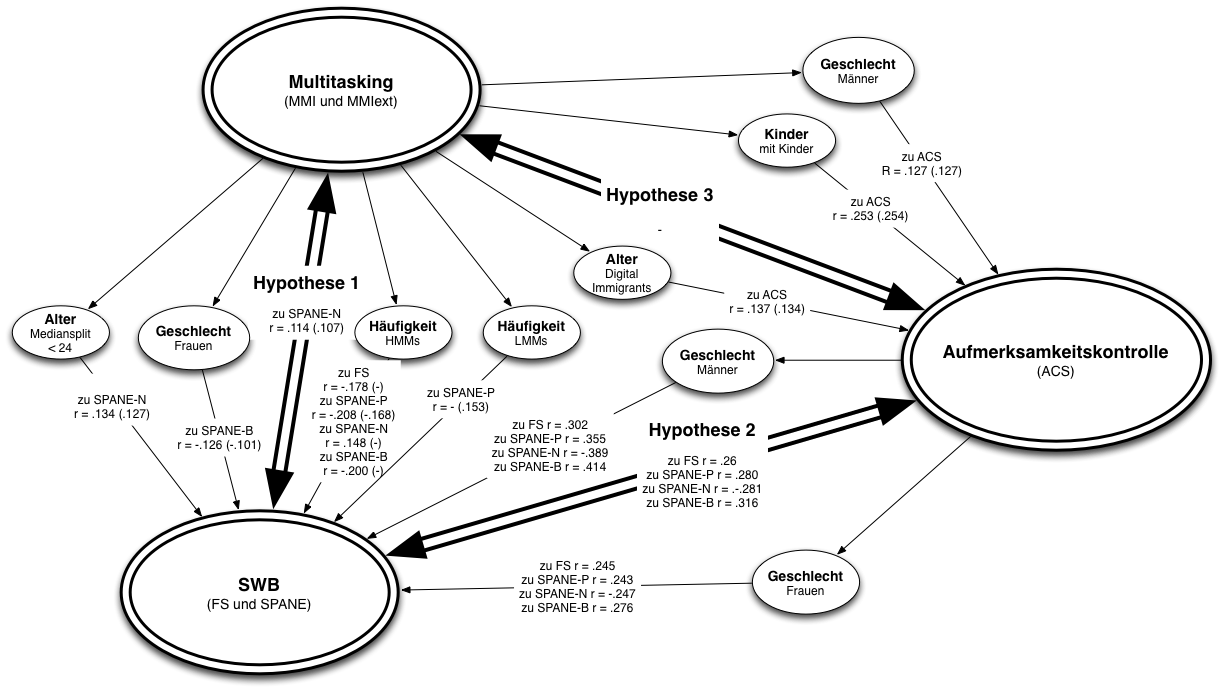
\includegraphics[scale=0.37]{images/grafiken/Zusammenhang_Zusammenfassung_v1.png}
     \caption{Zusammenhang der Variablen}
     \label{pic.ergebniss.zusammenfassung}
\end{figure}






%Diskussion
%%%%%%%%%%%%%%%%%%%%%%%%%%%%%%%%%%%%%%%%%%%%%%%%%%%%%%%%%%%%%%%%%
%_____________ ___    _____  __      __ 
%\____    /   |   \  /  _  \/  \    /  \  Institute of Applied
%  /     /    ~    \/  /_\  \   \/\/   /  Psychology
% /     /\    Y    /    |    \        /   Zuercher Hochschule 
%/_______ \___|_  /\____|__  /\__/\  /    fuer Angewandte Wissen.
%        \/     \/         \/      \/                           
%%%%%%%%%%%%%%%%%%%%%%%%%%%%%%%%%%%%%%%%%%%%%%%%%%%%%%%%%%%%%%%%%
%
% Project     : Bachelorarbeit
% Title       : Diskussion
% File        : diskussion.tex Rev. 00
% Date        : 06.12.2013
% Author      : Till J. Ernst
%
%%%%%%%%%%%%%%%%%%%%%%%%%%%%%%%%%%%%%%%%%%%%%%%%%%%%%%%%%%%%%%%%%
\glsresetall
% Kapitel Diskussion
\let\raggedsection\centering
\addchap{Diskussion}
\setcounter{chapter}{4}
\setcounter{section}{0}
\let\raggedsection\raggedright 

%####################################################
% Kapitel Beantwortung der Fragestellung
%####################################################
\section{Beantwortung der Fragestellung}\label{section.diskussion.fragestellung}
Im Folgenden wird die Fragestellung beantwortet, die bezüglich Übersichtlichkeit in eine Hauptfragestellung und drei Nebenfragestellungen unterteilt wurde. 
\par
\subsection{Hauptfragestellung.} Beeinflusst die Häufigkeit und die Fähigkeit bezogen auf Medien-Multitasking das subjektive Wohlbefinden von Studierenden?
\par
Gemäss den Ergebnissen dieser Studie konnte kein direkter Einfluss der Fähigkeit zur Aufmerksamkeitskontrolle auf das Medien-Multitasking Verhalten und das \gls{labelSWB} von Studierenden nachgewiesen werden. Es konnte jedoch nachgewiesen werden, dass die Fähigkeit zur Aufmerksamkeitskontrolle einen direkten Einfluss auf das \gls{labelSWB} haben. Dies wurde in der Unterfragestellung 2 beantwortet. Die geringe Korrelation zwischen dem Medien-Multitasking und dem subjektiven Wohlbefinden von $r=.114$ bei einem Signifikanzniveau von $p=.01$ wurde nicht durch die Fähigkeit zur Aufmerksamkeitskontrolle beeinflusst. Die Partialkorrelation mittels Fähigkeit zur Aufmerksamkeitskontrolle ergab ein $r_{par}=.141$ bei einem Signifikanzniveau von $p=.000$ und $df=1350$. Somit ist der direkte Zusammenhang zwischen Medien-Multitasking und dem \gls{labelSWB} nicht auf die Fähigkeit zur Aufmerksamkeitskontrolle zurückzuführen $r<r_{par}$. Für diese Fragestellung kann die Alternativhypothese 2 der Haupthypothese angenommen werden.

\subsection{Unterfragestellung 1} Welchen Einfluss hat die Häufigkeit von Medien-Multitasking auf das subjektive Wohlbefinden von Studierenden?
\par
Es wurde ein geringer signifikanter Zusammenhang zwischen der Variable für Medien-Multitasking und der Variable für das subjektive Wohlbefinden, in der Skala für negative Gefühle, von $r=.114$ bei einem Signifikanzniveau von $p=.01$ gefunden. Die Alternativhypothese der Arbeitshypothese 1 kann somit angenommen werden. Es scheint, dass die Häufigkeit von Medien-Multitasking einen negativen Einfluss auf das \gls{labelSWB} hat. \\
Wird eine Aufteilung der Stichprobe anhand des Geschlechts vorgenommen, so kann ein geringer negativ signifikanter Zusammenhang bei den weiblichen Teilnehmern ($N=951$) zwischen dem Medien-Multitasking und der Skala für positive Gefühle von $r=-.126$ bei einem Signifikanzniveau von $p=.01$ festgestellt werden. Bei den Männern ($N=401$) konnte kein Zusammenhang gefunden werden. Erfolgt die Unterteilung der Stichprobe anhand dem Multitasking Index der Personen, die stark Medien-Multitasking betreiben ($N=202$), können gering signifikante Zusammenhänge zwischen dem Medien-Multitasking und dem subjektiven Wohlbefinden ausgemacht werden. Die Auswirkung auf die Skala des  menschlichen Aufblühens ergab eine geringe negativ signifikante Korrelation von $r=-.178$ bei einem Signifikanzniveau von $p=.05$. Auf die Skala positive und negative Gefühle wurde eine geringe negativ signifikante Korrelation von $r=-.200$ bei einem Signifikanzniveau von $p=.01$ festgestellt. Auch für diese Zusammenhänge unterteilt nach Gruppen kann die Alternativhypothese der Arbeitshypothese 1 angenommen werden. Es scheint, dass Medien-Multitasking einen negativen Einfluss auf das subjektive Wohlbefinden hat.

\subsection{Unterfragestellung 2.} Welchen Einfluss hat die Fähigkeit zur Aufmerksamkeitskontrolle von Studierenden auf deren subjektives Wohlbefinden?

Zwischen der Fähigkeit zur Aufmerksamkeitskontrolle und dem \gls{labelSWB} konnten mehrere signifikante Ergebnisse gefunden werden. Ein geringer signifikanter Zusammenhang zwischen der Fähigkeit zur Aufmerksamkeitskontrolle und der Skala für das menschliche Aufblühen ($N=1364$) von $r=.265$ und ein mittlerer Zusammenhang zwischen der Aufmerksamkeitskontrolle und der Skala für positive und negative Gefühle ($N=1361$) von $r=.316$ bei einem Signifikanzniveau von $p=.01$. Die Alternativhypothese der Arbeitshypothese 2 kann somit angenommen werden. Die Fähigkeit zur Aufmerksamkeitskontrolle scheint einen geringen bis mittleren Einfluss auf das subjektive Wohlbefinden der Studierenden zu haben.

\subsection{Unterfragestellung 3.} Welchen Einfluss hat die Fähigkeit zur Aufmerksamkeitskontrolle auf das Medien-Multitasking-Verhalten von Studierenden?

Zwischen der Fähigkeit zur Aufmerksamkeitskontrolle und dem Medien-Multitasking konnte kein direkter Zusammenhang bei den Studierenden gefunden werden. Für diese Fragestellung muss somit die Nullhypothese der Arbeitshypothese 3 angenommen werden. Somit scheint es, dass die Fähigkeit zur Aufmerksamkeitskontrolle keinen Einfluss auf das Medien-Multitasking in dieser Untersuchung hat. \\
Jedoch lieferte die Unterteilung der Stichprobe anhand des Geschlechts ein geringer signifikanter Zusammenhang von $r=.127$ für die Kategorie Männer ($N=401$), zwischen dem Medien-Multitasking und der Aufmerksamkeitskontrolle bei einem Signifikanzniveau von $p=.05$. Einen weiteren gering signifikanten Zusammenhang zwischen der Fähigkeit zur Aufmerksamkeitskontrolle und dem Medien-Multitasking konnte bei der Aufteilung des Alters in Kategorien anhand Kohorten gefunden werden. Hierbei konnte bei der Kohorte Digital Immigrants ($N=216$) einen geringer Zusammenhang von $r=.137$ bei einem Signifikanzniveau von $p=.05$ gefunden werden. Die Aufteilung der Stichprobe anhand der Elternschaft ($N=79$), hatten die Probanden Kinder zum Zeitpunkt der Untersuchung, lieferte einen gering signifikanten Zusammenhang zwischen dem Medien-Multitasking und der Fähigkeit zur Aufmerksamkeitskontrolle von $r=.253$ bei einem Signifikanzniveau von $p=.05$. Für diese Unterteilung der Stichprobe in Kategorien kann die Nullhypothese der Arbeitshypothese 3 verworfen werden und die Alternativhypothese angenommen werden. Es scheint, dass die Fähigkeit zur Aufmerksamkeitskontrolle in spezifischen Gruppen einen Einfluss auf das Medien-Multitasking hat.

%####################################################
% Kapitel Interpretation
%####################################################
\section{TBD Interpretation}\label{section.diskussion.interpretation}
Unterteilung:
\begin{itemize}
    \item Fragestellung des Titels aufnehmen
    \item Unterschiede und Gemeinsamkeiten
    \begin{itemize}
        \item MT <-> SWB
        \item MT <-> ACS (Kinder)
        \item ACS <-> SWB
    \end{itemize}
    \item Einzelne Aspekte wie Gender herausgreiffen
    \item Umgang und Folgerund für die Praxis
    \item Fragestellung Titel beantworten
\end{itemize}

Beeinflusst nun das Multitasking das eigene Glück? Diese saloppe Frage, die im Titel aufgeworfen wird, nämlich ob das Multitasking das eigene Glück beeinflusst, wird im Folgenden zu beantworten versucht. Gemäss den Ergebnissen der Gruppe von Studierenden, die stark Medien-Multitasking betreiben (HMMs), konnte ein durchgehend geringer Zusammenhang zwischen \gls{labelMMT} und dem \gls{labelSWB} in allen \gls{labelSWB}-Skalen gefunden werden. Dies ist deshalb interessant, weil in der Studie von \citeA{Shih2013} kein Zusammenhang zwischen \gls{labelMMT} und \gls{labelSWB} nachgewiesen werden konnte. Diese Studie setzte einen speziell für diese Umfrage entwickelten Fragebogen \textit{\gls{labelSPD}} und den \gls{labelMUQ} ein, um die Medien-Aktivitäten von 138 Studierenden im Alter zwischen 18 und 43 Jahren zu erfassen. Für die Erfassung des \gls{labelSWB} wurden Fragebögen zu Sensation Seeking, dem \gls{labelFFM}, der Aufmerksamkeitskontrolle und Impulsivität erfasst. Im Gegensatz zur vorliegenden Studie, wurde die Aufmerksamkeitskontrolle als Teil vom \gls{labelSWB} verwendet \cite{Fergus2012}. Dies ist insofern nachzuvollziehen, als dass in der vorliegenden Studie ein direkter Zusammenhang zwischen der Aufmerksamkeitskontrolle und den \gls{labelSWB}-Skalen gefunden werden konnte. Die abweichenden Ergebnisse bezüglich Auswirkung auf das \gls{labelSWB} könnten auf die geringere Stichprobengrösse und die unterschiedlichen Erhebungsinstrumente des \gls{labelSWB} zurückzuführen sein. Beide Studien erfassten die Mediennutzung von Studierenden und setzten dafür den \gls{labelMUQ} ein. Bei der Studie von \citeauthor{Shih2013} kam zusätzlich der \gls{labelSPD} zu Zuge, der die Mediennutzung tagebuchartig erfasste. Der \gls{labelMUQ} wurde für diese Studie angepasst, indem er anstelle der eingeschätzten Mediennutzung pro Woche, diese pro Tag erfasste. Neben dem Unterschied, dass \citeA{Shih2013} keine Auswirkung auf das \gls{labelSWB} gefunden hatte, wurde ein weiterer Unterschied bezüglich Mediennutzung in Stunden pro Woche sichtbar: In der vorliegenden Studie konnte eine durchschnittliche Mediennutzung von 49.28 Stunden pro Woche gemessen werden. Bei der Studie von \citeauthor{Shih2013} war die durchschnittliche Nutzung beim \gls{labelMUQ} mit 97.73 Stunden angegeben. Dieser Unterschied könnte darauf beruhen, dass die Selbsteinschätzung der Mediennutzung für eine Woche weniger akkurat ist, als für die Einschätzung der Nutzung pro Tag, wie es für die vorliegende Studie gemacht wurde. Dies würde für die vorliegende Arbeit sprechen. Es könnte aber auch sein, da der \gls{labelSPD} im Ablauf vor dem \gls{labelMUQ} durchgeführt wurde, dass die Probanden die Selbsteinschätzung genauer vornehmen konnten, da durch den Medienaufschrieb mittels Tagebuch bereits ein Priming stattgefunden hatte und sie deshalb eine realistischere Schätzung abgeben konnten, was gegen das vorliegende Vorgehen sprechen würde. Diese Unterschiede bezüglich der Mediennutzung pro Woche könnte auch der Grund für die Unterschiedlichen Resultate des $MMI$ sein: Die vorliegend Studie erfasste 45 Personen (3.3\%), die kein Medien-Multitasking betreiben, wobei die Studie von \citeA{Shih2013} nur Personen erfasste, die Medien-Multitasking betrieben (Minimum $MMI = 0.49$). Werden die Resultate der Mediennutzung mit der Umfrage der Kaiser Family Foundation verglichen, so fällt auch hier ein Unterschied auf \citeA{Rideout2010}. Gemäss \citeA{Wallis2010} betreiben 15 bis 20\% der jugendlichen Amerikaner zwischen 8 und 18 Jahren kein \gls{labelMMT}. Dieser Unterschied könnte sich damit erklären lassen, dass die vorliegende Stichprobe ausschliesslich Studierende beinhaltet, die Medien aufgrund ihres Studiums nutzen (z.B.: Computer) und deshalb eher zu Multitasking neigen, da sie den Zugang zu \gls{labelMMT} über das Studium finden. \citeA{Rideout2010} und ihr Team haben über 2000 amerikanische Jugendlichen zu ihrem Medienkonsum befragt und sind auf eine Mediennutzungsdauer von 7.5 Stunden pro Tag gekommen. Dieses Resultat deckt sich annähernd mit dem Resultat von 49.3 Stunden pro Woche der vorliegenden Studie, was ein Tagesdurchschnitt von 7.04 Stunden ergibt. Wobei hier zu erwähnen ist, dass die Studie um \cite<ebda.,>{Rideout2010} zwischen der reinen Mediennutzung und der simultanen Mediennutzung durch Multitasking unterscheidet. In der vorliegenden Studie wurde die Mediennutzung im Total erfasst (inkl. Multitasking). Aus dieser Perspektive wenden die Probanden der Kaiser Familiy Foundation 10.75 Stunden Mediennutzung inklusive Multitasking auf. Diese Differenz von über 3 Stunden könnte sich anhand dem Alter der Probanden erklären lassen: Je Jünger, desto mehr Multitasking wird angewendet. Diese Hypothese müsste jedoch anhand der vorliegenden Daten weiter untersucht werden. Einen weiterer Grund für die unterschiedliche Resultate könnte aufgrund der unterschiedlichen Nationalitäten entstanden sein. Eventuell wenden amerikanische Jugendliche mehr \gls{labelMMT} an als Studierende in der Schweiz. Wie bereits bei der Studie um \citeA{Shih2013} könnte die unterschiedliche Mediennutzung aufgrund der verschiedenen Erhebungsinstrumente basieren (Tagebuch gegenüber Selbsteinschätzung der Nutzung in Minuten und Tag). Die Selbsteinschätzung mittels \gls{labelMUQ} könnte gegenüber einem Medien-Tagebuch ungenaue Werte liefern \cite{Greenberg2005}.\\

MT <-> ACS
\par
ACS <-> SWB
\par
Einschränkungen: 

Folgende Themen sollen in diesem Kapitel behandelt werden (TBD):
\begin{itemize}
    \item Bestehende Forschung
    \item Folgerung für die Praxis
    \item HMM stärkere Auswirkung auf das SWB -> zusätzliche Hinweise zu bestehender Theorie
    \item Geschlecht (w) stärkere Auswirkung auf SWB -> nicht naheliegend; in der Theorie Unterschiede zwischen w und m nicht bekannt
    \item unerwartetes Ergebnis der Studenten, die unter (oder gleich) 24 Jahre alt waren -> negative Auswirkung auf das SWB
    \item keine direkte Auswirkung auf die Fähigkeit zur Aufmerksamkeitskontrolle. Jedoch wirken sich Kinder, das Geschlecht und das Alter auf diese Komponente aus
    \item direkter Zusammenhang zwischen Fähigkeit zur Aufmerksamkeitskontrolle und SWB -> anhand der Theorie der positiven Psychologie (Flow) erklärbar
    \item Von Mail Rivka: Was mir gerade vorher beim Einscannen noch aufgefallen ist: Im Titel heisst es ja „Beeinflusst Multitasking das eigene Glück?“. Diese Frage nimmst du nirgends auf in der Arbeit bzw. nur in einer ganz anderen / wissenschaftlichen Sprache. Allenfalls könnte man diese umgangssprachliche Frage in der Einleitung bzw. beim Ziel und/oder bei der Zusammenfassung der Ergebnisse noch einbringen. Im Stile von: „Die saloppe Frage, welche im Titel dieser Arbeit aufgeworfen wird, nämlich ob das Multitasking das eigene Glück beeinflusst, kann damit wie folgt beantwortet werden: ….“.
\end{itemize}

 Dieses Ergebnis ist insofern interessant, da es in diesem Bereich wenig existierende Studien gibt und sich diese gegenseitig eher widersprechen \cite{Pea2012, Shih2013}. Durch dieses konnte zumindest dargestellt werden, dass die Häufigkeit von Medien-Multitasking bei Studierenden eine mögliche Auswirkung auf das subjektive Wohlbefinden hat. Ob es sich beim Medien-Multitasking um die Auslösende Variable handelt oder ob eine weitere, verdeckte Variable für diesen Zusammenhang verantwortlich ist, müssen weiterführende Studien erst noch belegen. 
%####################################################
% Kapitel Methodenkritik
%####################################################
\section{TBD Methodenkritik}\label{section.diskussion.methodenkritik}
Folgende Themen sollen in diesem Kapitel behandelt werden (TBD):
\begin{itemize}
    \item $MMI_{ext}$ und $MMI$ einmal mit SMS als Hauptmedium und einmal ohne SMS als Hauptmedium sondern nur als Nebenmedium (originale Version). Dies, da die Nutzung pro Tag und Minute erfragt wurde (orig. in Stunden pro Woche)
    \item MUQ - Alle Medien werden gleich bewertet (z.B.: sms und tv)
    \item Im Onlinefragebogen bei der Sektion MUQ wurden bereits vorgewählte Antworten bei den simultan verwendeten Medien verwendet (ein allfälliges Nebenmedium wird nicht verwendet)
    \item ACS - Selbstbeurteilung der Fähigkeit zur Aufmerksamkeitskontrolle (Frage bezüglich Validität)
\end{itemize}


%####################################################
% Kapitel Ausblick
%####################################################
\section{Ausblick}\label{section.diskussion.ausblick}
Die Ergebnisse dieser Studie liefern eine gute Grundlage für weitere Untersuchungen im Bereich des Medien-Multitasking. Durch die grosse Stichprobe können weitere Zusammenhänge und Eigenschaften des Medien-Multitasking Verhaltens untersucht werden, die in dieser Studie keinen Platz fanden. Die Resultate lassen die Annahme zu, dass es einen Zusammenhang zwischen dem Medien-Multitasking und dem subjektiven Wohlbefinden geben könnte. Dieser Bereich benötigt zusätzliche Forschung und eine vertiefte Auseinandersetzung mit dem Thema. Die fortführende Auseinandersetzung mit der Fähigkeit zur Aufmerksamkeitskontrolle und die Auswirkung von Multitasking auf diese benötigt weitere Ergebnisse. Ein spannendes Thema könnte die Befassung mit möglichen Einflussfaktoren neben der Fähigkeit zur Aufmerksamkeitskontrolle auf das subjektive Wohlbefinden sein. Zum Beispiel könnten soziale Faktoren wie Umgebung, Beziehung oder auch Bildung mögliche Wirkfaktoren für das Multitasking verhalten und die Auswirkung auf das subjektive Wohlbefinden darstellen. Ebenso ist vorstellbar, dass das subjektive Wohlbefinden in weitere Teilbereiche unterteilt wird, um eine allfällige Beeinflussung des Multitasking aufzuzeigen. Eine zentrale Rolle in dieser Diskussion scheint der Langzeitauswirkung von Medien-Multitasking zuzukommen. Wie wirken sich diese Medien-Präferenzen auf unser Gehirn und deren Areale aus. Tendiert unser Gehirn dazu, umgebungsbedingte Einflüsse zu adaptieren oder stossen wir an unsere Kapazitäts- und Leistungsgrenzen, was unsere kognitiven Fähigkeiten anbelangt. Diese notwendigen Untersuchungen sollen dazu beitragen, den künftigen Umgang mit Medien und wie Medien technologisch umgesetzt werden, zu erleichtern. Eine auf unsere Bedürfnisse und Fähigkeiten abgestimmte Medienwelt, die unser Potential anregt und unsere Fähigkeiten erweitert, ist einer von Reizen überfluteten, teilweise überfordernden und stressverursachenden Umwelt definitiv vorzuziehen. 


% -----------------------------------

% Literaturverzeichnis
%%%%%%%%%%%%%%%%%%%%%%%%%%%%%%%%%%%%%%%%%%%%%%%%%%%%%%%%%%%%%%%%%
%_____________ ___    _____  __      __ 
%\____    /   |   \  /  _  \/  \    /  \  Institute of Applied
%  /     /    ~    \/  /_\  \   \/\/   /  Psychology
% /     /\    Y    /    |    \        /   Zürcher Hochschule 
%/_______ \___|_  /\____|__  /\__/\  /    fuer Angewandte Wissen.
%        \/     \/         \/      \/                           
%%%%%%%%%%%%%%%%%%%%%%%%%%%%%%%%%%%%%%%%%%%%%%%%%%%%%%%%%%%%%%%%%
%
% Project     : Bachelorarbeit
% Title       : 
% File        : literatur.tex Rev. 00
% Date        : 06.12.2013
% Author      : Till J. Ernst
%
%%%%%%%%%%%%%%%%%%%%%%%%%%%%%%%%%%%%%%%%%%%%%%%%%%%%%%%%%%%%%%%%%
% Bibliographie in APA Style
%\nocite{*} %-> führ alle Referenzen im Bibtex-Lib auf
\bibliographystyle{apacite}
\bibliography{Bibliography}{}

%mit biber
%\begin{refsection}[biblatex-apa-test-references]
%\nocite{*}
%\end{refsection}
%\newpage
%\printbibliography


%\end{RaggedRight}

%%%%%%%%%%%%%%%%%%%%%%%%%%%%%%%%%%%%%%%%%%%%%%%%%%%%%%%%%%%%% 
%% ANHANG 
%% Anhang erscheint nicht im Inhaltsverzeichnis
%%%%%%%%%%%%%%%%%%%%%%%%%%%%%%%%%%%%%%%%%%%%%%%%%%%%%%%%%%%%%
\pagenumbering{arabic}
\appendix 
\renewcommand{\appendixname}{Anhang} 
\renewcommand{\appendixtocname}{\appendixname} 
\addappheadtotoc % Anhang in Hauptinhaltsverzeichnis aufnehmen
\addtocontents{toc}{\protect\setcounter{tocdepth}{-1}} % die kommenden Anhänge erscheinen nicht im Inhaltsverzeichnis 

%%%%%%%%%%%%%%%%%%%%%%%%%%%%%%%%%%%%%%%%%%%%%%%%%%%%%%%%%%%%%%%%%
%_____________ ___    _____  __      __ 
%\____    /   |   \  /  _  \/  \    /  \  Institute of Applied
%  /     /    ~    \/  /_\  \   \/\/   /  Psychology
% /     /\    Y    /    |    \        /   Zuercher Hochschule 
%/_______ \___|_  /\____|__  /\__/\  /    fuer Angewandte Wissen.
%        \/     \/         \/      \/                           
%%%%%%%%%%%%%%%%%%%%%%%%%%%%%%%%%%%%%%%%%%%%%%%%%%%%%%%%%%%%%%%%%
%
% Project     : Bachelorarbeit
% Title       : 
% File        : Rev. 00
% Date        : 06.12.2013
% Author      : Till J. Ernst
%
%%%%%%%%%%%%%%%%%%%%%%%%%%%%%%%%%%%%%%%%%%%%%%%%%%%%%%%%%%%%%%%%%
\glsresetall
\let\raggedsection\centering 
\chapter*{Anhang}\label{chap.appendixStart}
\let\raggedsection\raggedright 
\begin{RaggedRight}
tbd
\end{RaggedRight}

%%%%%%%%%%%%%%%%%%%%%%%%%%%%%%%%%%%%%%%%%%%%%%%%%%%%%%%%%%%%%%%%%
%_____________ ___    _____  __      __ 
%\____    /   |   \  /  _  \/  \    /  \  Institute of Applied
%  /     /    ~    \/  /_\  \   \/\/   /  Psychology
% /     /\    Y    /    |    \        /   Zuercher Hochschule 
%/_______ \___|_  /\____|__  /\__/\  /    fuer Angewandte Wissen.
%        \/     \/         \/      \/                           
%%%%%%%%%%%%%%%%%%%%%%%%%%%%%%%%%%%%%%%%%%%%%%%%%%%%%%%%%%%%%%%%%
%
% Project     : Bachelorarbeit
% Title       : 
% File        : Rev. 00
% Date        : 06.12.2013
% Author      : Till J. Ernst
%
%%%%%%%%%%%%%%%%%%%%%%%%%%%%%%%%%%%%%%%%%%%%%%%%%%%%%%%%%%%%%%%%%
\glsresetall

\let\raggedsection\centering 
\chapter{Liste der angeschriebenen Schulen}\label{chap.appendix_schulListe}
\let\raggedsection\raggedright 
\begin{RaggedRight}
% Liste der Schulen
Im Folgenden werden die für diese Studie angeschriebenen Universitäten und Fachhochschulen aufgelistet. Trotz einzeln angeschriebener Departemente innerhlab der Schulen wurden diese aus Gründen der Darstellung weggelassen.\par
\textbf{Liste der angeschriebenen Universitäten:}
\begin{itemize}
    \item Basel
    \item Bern
    \item Luzern
    \item St. Gallen
    \item Zürich
\end{itemize}
\textbf{Liste der Fachhochschulen:}
\begin{itemize}
    \item Berner Fachhochschule
    \item Hochschule Luzern
    \item Zürcher Fachhochschule
    \begin{itemize}
        \item Zürcher Hochschule für Angewandte Wissenschaften
        \item Zürcher Hochschule der Künste
        \item PH Zürich
        \item HWZ Hochschule für Wirtschaft
    \end{itemize}
    \item Fachhochschule Ostschweiz
    \item Fachhochschule Nordwestschweiz 
    \item Kalaidos Fachhochschule Schweiz
\end{itemize}

\end{RaggedRight}

%%%%%%%%%%%%%%%%%%%%%%%%%%%%%%%%%%%%%%%%%%%%%%%%%%%%%%%%%%%%%%%%%
%_____________ ___    _____  __      __ 
%\____    /   |   \  /  _  \/  \    /  \  Institute of Applied
%  /     /    ~    \/  /_\  \   \/\/   /  Psychology
% /     /\    Y    /    |    \        /   Zuercher Hochschule 
%/_______ \___|_  /\____|__  /\__/\  /    fuer Angewandte Wissen.
%        \/     \/         \/      \/                           
%%%%%%%%%%%%%%%%%%%%%%%%%%%%%%%%%%%%%%%%%%%%%%%%%%%%%%%%%%%%%%%%%
%
% Project     : Bachelorarbeit
% Title       : 
% File        : Rev. 00
% Date        : 06.12.2013
% Author      : Till J. Ernst
%
%%%%%%%%%%%%%%%%%%%%%%%%%%%%%%%%%%%%%%%%%%%%%%%%%%%%%%%%%%%%%%%%%
\glsresetall

\let\raggedsection\centering 
\chapter{Anhang C}\label{chap.appendix_mailing}
\let\raggedsection\raggedright 
\begin{RaggedRight}
TBD
\end{RaggedRight}

%%%%%%%%%%%%%%%%%%%%%%%%%%%%%%%%%%%%%%%%%%%%%%%%%%%%%%%%%%%%%%%%%
%_____________ ___    _____  __      __ 
%\____    /   |   \  /  _  \/  \    /  \  Institute of Applied
%  /     /    ~    \/  /_\  \   \/\/   /  Psychology
% /     /\    Y    /    |    \        /   Zuercher Hochschule 
%/_______ \___|_  /\____|__  /\__/\  /    fuer Angewandte Wissen.
%        \/     \/         \/      \/                           
%%%%%%%%%%%%%%%%%%%%%%%%%%%%%%%%%%%%%%%%%%%%%%%%%%%%%%%%%%%%%%%%%
%
% Project     : Bachelorarbeit
% Title       : 
% File        : Rev. 00
% Date        : 06.12.2013
% Author      : Till J. Ernst
%
%%%%%%%%%%%%%%%%%%%%%%%%%%%%%%%%%%%%%%%%%%%%%%%%%%%%%%%%%%%%%%%%%
\glsresetall

\let\raggedsection\centering 
\chapter{Aushang Rekrutierung}\label{chap.appendix_aushang}
\let\raggedsection\raggedright 
\begin{RaggedRight}
% Aushang
Der Flyer für die Teilnahme an der Umfrage für den Aushang am Schwarzen Brett wurde zusammen mit dem Mailing versendet. Dieser Flyer ist in angepasster Form abgebildet.
\par
%\begin{figure}[h]
%    \centering
%    
\includegraphics[scale=0.5]{images/anhang/WeWantYou.jpeg}
%\end{figure}
\textbf{Umfrage und Wettbewerb: Gutscheine zu gewinnen!}\\
Liebe Studierende

Ich benötige Studierende, die meinen Fragebogen zu Medien-Multitasking und subjektivem Wohlbefinden für meine Bachelorarbeit ausfüllen. Der Fragebogen wird in etwa 10 bis 15 Minuten von Eurer Zeit in Anspruch nehmen. Im Anschluss an die Fragen könnt Ihr an einem Wettbewerb teilnehmen, in dem Ihr Gutscheine vom Athleticum Sportsmarket gewinnen könnt (2 x CHF 100.- und 4 x CHF 40.-).

Die Umfrage findet Ihr unter: \url{http://www.unipark.de/uc/multitasking_and_swb/} oder mittels unten stehenden QR Code (siehe Kurzanleitung nach dem Code).

Ich würde mich freuen, wenn Ihr mich in meiner Arbeit unterstützen könnt und wünsche Euch ein gutes erfolgreiches neues Semester!

Mit den besten Grüssen
Till Ernst\\
Dipl. Ing. FH Software und stud. Bachelor in applied Psychology\\
Mail: \href{mailto:ernsttil@students.zhaw.ch}{ernsttil@students.zhaw.ch}\\
\begin{figure}[h]
    \centering
    
\includegraphics[scale=0.5]{images/anhang/umfrage_qr_code.png}
\end{figure}
Code mit Mobile-Telefon und QR-Reader-App scannen (z.B.: QR-Reader für iPhone oder QR-Droid für Android).
\end{RaggedRight}

%%%%%%%%%%%%%%%%%%%%%%%%%%%%%%%%%%%%%%%%%%%%%%%%%%%%%%%%%%%%%%%%%
%_____________ ___    _____  __      __ 
%\____    /   |   \  /  _  \/  \    /  \  Institute of Applied
%  /     /    ~    \/  /_\  \   \/\/   /  Psychology
% /     /\    Y    /    |    \        /   Zuercher Hochschule 
%/_______ \___|_  /\____|__  /\__/\  /    fuer Angewandte Wissen.
%        \/     \/         \/      \/                           
%%%%%%%%%%%%%%%%%%%%%%%%%%%%%%%%%%%%%%%%%%%%%%%%%%%%%%%%%%%%%%%%%
%
% Project     : Bachelorarbeit
% Title       : 
% File        : Rev. 00
% Date        : 06.12.2013
% Author      : Till J. Ernst
%
%%%%%%%%%%%%%%%%%%%%%%%%%%%%%%%%%%%%%%%%%%%%%%%%%%%%%%%%%%%%%%%%%
\glsresetall

\let\raggedsection\centering 
\chapter{Media Use Questionnaire -- MUQ}\label{chap.appendix_mediaUseQuestionnaire}
\let\raggedsection\raggedright 
\begin{RaggedRight}
%Media Use Questionnaire
Für die Erfassung des \textit{Media Multitasking Index (MMI)} von \citeA{Ophir2009} wurde der aus dem englisch sprachigen Raum stammende Fragebogen \textit{Media Use Questionnaire} aus dem Englischen ins Deutsche übersetzt.
Die Bewertung der Medien-Multitasking-Matrix (siehe \nameref{section.erhebungsinstrumente}) erfolgt mittels folgender Skala: 1 = meistens (engl.: most of the time); 0.67 = etwas (engl.: some of the time); 0.33 = wenig (engl.: a little of the time); 0 = nie (engl.: never).  \\

%Tabelle
\begin{center}
    \begin{longtable}[t]{|l|p{6.6 cm}|p{6.6 cm}|}
    \caption{Medie Use Questionnaire - Medienübersetzung} \\ \hline
        \textbf{Nr.} & \textbf{Englisch} & \textbf{Deutsch} \\ \hline
        \endfirsthead
        \hline
        \textbf{Nr.} & \textbf{Englisch} & \textbf{Deutsch} \\ \hline
        \endhead 
        & \multicolumn{2}{|c|}{Fortsetzung auf der nächsten Seite $...$ } \\ \hline
        \endfoot
        \hline
        \endlastfoot
        1 & print media & Druckmedien \\
        2 & television & Fernsehen \\
        3 & computer-based video (such as YouTube or online television episodes) & Online Video (wie zum Beispiel Youtube) \\
        4 & music & Musik \\
        5 & nonmusic audio & Nicht-musikalische Audiomedien (z.B. Hörbücher, Podcast, etc.) \\
        6 & video or computer games & Video oder Computer Games \\
        7 & telephone and mobile phone voice calls & Telefonieren (Mobil- und / oder Festnetz) \\
        8 & instant messaging & Instant Messaging (z.B. Skype, Windows Live Messenger, Yahoo Messenger, etc.) \\
        9 & SMS (text messaging) & SMS (Textnachrichten) \\
        10 & email & Email \\
        11 & web surfing & Internet-Surfen \\
        12 & other computer-based application  & Andere Computerbasierte-Tätigkeiten (z.B. Word, Videobearbeitung, programmieren, etc.) \\
        \end{longtable}
	\label{tab.muqUebersetzung}
\end{center}



\end{RaggedRight}

%%%%%%%%%%%%%%%%%%%%%%%%%%%%%%%%%%%%%%%%%%%%%%%%%%%%%%%%%%%%%%%%%
%_____________ ___    _____  __      __ 
%\____    /   |   \  /  _  \/  \    /  \  Institute of Applied
%  /     /    ~    \/  /_\  \   \/\/   /  Psychology
% /     /\    Y    /    |    \        /   Zuercher Hochschule 
%/_______ \___|_  /\____|__  /\__/\  /    fuer Angewandte Wissen.
%        \/     \/         \/      \/                           
%%%%%%%%%%%%%%%%%%%%%%%%%%%%%%%%%%%%%%%%%%%%%%%%%%%%%%%%%%%%%%%%%
%
% Project     : Bachelorarbeit
% Title       : 
% File        : Rev. 00
% Date        : 06.12.2013
% Author      : Till J. Ernst
%
%%%%%%%%%%%%%%%%%%%%%%%%%%%%%%%%%%%%%%%%%%%%%%%%%%%%%%%%%%%%%%%%%
\glsresetall

\let\raggedsection\centering 
\chapter{Attentional Control Scale -- ACS}\label{chap.appendix_attentionalControlScale}
\let\raggedsection\raggedright 
\begin{RaggedRight}

% Attentional Control Scale
Die Bewertung der Elemente des aus dem Englisch stammenden Fragebogens \textit{Attentional Control Scale - (ACS)} \cite{Derryberry2002} erfolgte mittels vierstufigen Skala: 1 = fast nie (engl.: almost never); 2 = manchmal (engl.: sometimes); 3 = oft (engl.: often); 4 = immer (engl.: always).\newline
Im Folgenden werden die einzelnen Elemente inkl. englischer Übersetzung aufgelistet. (R) steht für invertiert bewertete Elemente:
\begin{center}
    \begin{longtable}[t]{|l|p{6.6 cm}|p{6.6 cm}|}
    \caption{Attentional Control Scale - Übersetzung} \\ \hline
        \textbf{Nr.} & \textbf{Englisch} & \textbf{Deutsch} \\ \hline
        \endfirsthead
        \hline
        \textbf{Nr.} & \textbf{Englisch} & \textbf{Deutsch} \\ \hline
        \endhead 
        & \multicolumn{2}{|c|}{Fortsetzung auf der nächsten Seite $...$ } \\ \hline
        \endfoot
        \hline
        \endlastfoot
        1 & It’s very hard for me to concentrate on a difficult task when there are noises around. (R) & In einer lauten Umgebung habe ich Mühe, mich auf eine schwierige Aufgabe zu konzentrieren.\\ 
        2 & When I need to concentrate and solve a problem, I have trouble focusing my attention. (R) & Wenn mich auf die Lösung eines Problems konzentrieren muss, habe ich Mühe meine Aufmerksamkeit zu fokussieren.\\ 
        3 & When I am working hard on something, I still get distracted by events around me. (R) & Wenn ich mich intensiv mit etwas beschäftige, werde ich durch Ereignisse um mich herum abgelenkt.\\ 
        4 & My concentration is good even if there is music in the room around me. & Musik im gleichen Raum stört meine Konzentration nicht.\\
        5 & When concentrating, I can focus my attention so that I become unaware of what’s going on in the room around me. & Wenn ich mich auf etwas konzentriere,  so kann ich meine Aufmerksamkeit derart fokussieren, dass ich alles um mich herum vergesse. \\
        6 & When I am reading or studying, I am easily distracted if there are people talking in the same room. (R) & Wenn ich lesen oder etwas lernen muss, lasse ich mich leicht ablenken, wenn Leute im selben Raum miteinander sprechen. \\
        7 & When trying to focus my attention on something, I have difficulty blocking out distracting thoughts. (R) & Wenn ich meine Aufmerksamkeit auf etwas zu konzentrieren versuche, so habe ich Schwierigkeiten ablenkende Gedanken abzublocken. \\
        8 & I have a hard time concentrating when I’m excited about something. (R) & Ich habe Mühe, mich zu konzentrieren, wenn ich aufgeregt bin. \\
        9 & When concentrating I ignore feelings of hunger or thirst. & Wenn ich mich konzentriere vergesse ich, dass ich durstig oder hungrig bin. \\
        10 & I can quickly switch from one task to another. & Ich kann rasch von einer Aufgabe zur nächsten Aufgabe wechseln. \\
        11 & It takes me a while to get really involved in a new task. (R) & Es dauert eine Weile, bis ich mich in eine neue Aufgabe eingearbeitet habe. \\
        12 & It is difficult for me to coordinate my attention between the listening and writing required when taking notes during lectures. (R) & Es bereitet mir Schwierigkeiten, meine Aufmerksamkeit zwischen dem Zuhören und dem Niederschreiben von Informationen während der Vorlesung zu koordinieren. \\
        13 & I can become interested in a new topic very quickly when I need to. & Wenn erforderlich, kann ich mich leicht für ein neues Thema begeistern.  \\
        14 & It is easy for me to read or write while I’m also talking on the phone. & Es fällt mir leicht, während eines Telefonats gleichzeitig zu lesen oder zu schreiben.  \\
        15 & I have trouble carrying on two conversations at once. (R) & Es bereitet mir Mühe, zwei verschiedene Gespräche gleichzeitig zu führen. \\
        16 & I have a hard time coming up with new ideas quickly. (R) & Es fällt mir schwer, spontan auf neue Ideen zu kommen. \\
        17 & After being interrupted or distracted, I can easily shift my attention back to what I was doing before. & Nachdem ich abgelenkt oder unterbrochen wurde, kann ich meine Aufmerksamkeit mühelos auf die vorherige Arbeit lenken. \\
        18 & When a distracting thought comes to mind, it is easy for me to shift my attention away from it. & Wenn mir ein störender Gedanke in den Sinn kommt, so kann ich ihn ohne grosse Mühe wieder vergessen.  \\
        19 & It is easy for me to alternate between two different tasks. & Es fällt mir leicht, zwischen zwei unterschiedlichen Tätigkeiten hin und her zu wechseln. \\
        20 & It is hard for me to break from one way of thinking about something and look at it from another point of view. (R) & Es fällt mir schwer, mich von meiner bisherigen Denkweise zu lösen und einen Sachverhalt von einer anderen Seite zu betrachten. \\ \hline
    \end{longtable}
	\label{tab:AcsUebersetzung}
\end{center}
\end{RaggedRight}

%%%%%%%%%%%%%%%%%%%%%%%%%%%%%%%%%%%%%%%%%%%%%%%%%%%%%%%%%%%%%%%%%
%_____________ ___    _____  __      __ 
%\____    /   |   \  /  _  \/  \    /  \  Institute of Applied
%  /     /    ~    \/  /_\  \   \/\/   /  Psychology
% /     /\    Y    /    |    \        /   Zuercher Hochschule 
%/_______ \___|_  /\____|__  /\__/\  /    fuer Angewandte Wissen.
%        \/     \/         \/      \/                           
%%%%%%%%%%%%%%%%%%%%%%%%%%%%%%%%%%%%%%%%%%%%%%%%%%%%%%%%%%%%%%%%%
%
% Project     : Bachelorarbeit
% Title       : 
% File        : Rev. 00
% Date        : 06.12.2013
% Author      : Till J. Ernst
%
%%%%%%%%%%%%%%%%%%%%%%%%%%%%%%%%%%%%%%%%%%%%%%%%%%%%%%%%%%%%%%%%%
\glsresetall

\let\raggedsection\centering 
\chapter{Übersetzung -- Flourishing Scale}\label{chap.appendix_fs}
\let\raggedsection\raggedright 
\begin{RaggedRight}
% Flourishing Scale
Die Skala für die Erfassung des menschlichen Wohls (engl.: Flourishing Scale - FS) \cite{Diener:2010} besteht aus einer einleitenden Anweisung und den zugehörenden Fragebogen-Elemente. Bewertet werden die Elemente auf einer siebenstufigen Skala: 1 = trifft überhaupt nicht zu (engl.: strongly disagree); 2 = trifft nicht zu (engl.: disagree); 3 = trifft kaum zu (engl.: slightly disagree); 4 = gemischt oder weder Zustimmung noch Ablehnung (engl.: mixed or neither agree nor disagree); 5 = trifft etwas zu (engl.: slightly agree); 6 = trifft zu (engl.: agree); 7 = trifft voll und ganz zu (engl.: strongly agree).

% Table
\begin{center}
    \begin{longtable}[t]{|p{15 cm}|}
    \caption{Übersetzung Anweisung -- Flourishing Scale} \\ \hline
        \textbf{Englisch} \\ \hline
        Below are eight statements with which you may agree or disagree. Using the 1–7 scale below, indicate your agreement with each item by indicating that response for each statement. \\ \hline
        \textbf{Deutsch} \\ \hline 
        Unten findest Du acht Aussagen, denen Du zustimmen oder widersprechen kannst. Bewerte jede Aussage auf einer Skala von 1 bis 7 (1 = trifft überhaupt nicht zu bis 7 = trifft voll und ganz zu). \\ \hline   
    \end{longtable}
	\label{tab:FsAnweisung}
\end{center}

% Table
\begin{center}
    \begin{longtable}[t]{|p{0.8 cm}|p{6.6 cm}|p{6.6 cm}|}
    \caption{Übersetzung Elemente -- Flourishing Scale} \\ \hline
        \textbf{Nr.} & \textbf{Englisch} & \textbf{Deutsch} \\ \hline
        \endfirsthead
        \hline
        \textbf{Nr.} & \textbf{Englisch} & \textbf{Deutsch} \\ \hline
        \endhead 
        & \multicolumn{2}{|c|}{Fortsetzung auf der nächsten Seite $...$ } \\ \hline
        \endfoot
        \hline
        \endlastfoot
        1 & I lead a purposeful and meaningful life. & Ich führe ein zielgerichtetes und sinnvolles Leben.\\
        2 & My social relationships are supportive and rewarding. & Meine sozialen Beziehungen stärken und bereichern mich. \\
        3 & I am engaged and interested in my daily activities. & Ich bin engagiert und interessiere mich für meine täglichen Aktivitäten.\\
        4 & I actively contribute to the happiness and well-being of others. & Ich trage aktiv zum Glück und zum Wohlbefinden anderer bei.\\
        5 & I am competent and capable in the activities that are important to me. & In den Aktivitäten, die mir wichtig sind, bin ich kompetent und fähig.\\
        6 & I am a good person and live a good life. & Ich bin ein guter Mensch und ich führe ein gutes Leben. \\
        7 & I am optimistic about my future. & Ich bin optimistisch, was meine Zukunft betrifft.\\
        8 & People respect me. & Die Leute respektieren mich.\\        
    \end{longtable}
	\label{tab:FsElemente}
\end{center}

\end{RaggedRight}

%%%%%%%%%%%%%%%%%%%%%%%%%%%%%%%%%%%%%%%%%%%%%%%%%%%%%%%%%%%%%%%%%
%_____________ ___    _____  __      __ 
%\____    /   |   \  /  _  \/  \    /  \  Institute of Applied
%  /     /    ~    \/  /_\  \   \/\/   /  Psychology
% /     /\    Y    /    |    \        /   Zuercher Hochschule 
%/_______ \___|_  /\____|__  /\__/\  /    fuer Angewandte Wissen.
%        \/     \/         \/      \/                           
%%%%%%%%%%%%%%%%%%%%%%%%%%%%%%%%%%%%%%%%%%%%%%%%%%%%%%%%%%%%%%%%%
%
% Project     : Bachelorarbeit
% Title       : 
% File        : Rev. 00
% Date        : 06.12.2013
% Author      : Till J. Ernst
%
%%%%%%%%%%%%%%%%%%%%%%%%%%%%%%%%%%%%%%%%%%%%%%%%%%%%%%%%%%%%%%%%%
\glsresetall

\let\raggedsection\centering 
\chapter{Anhang H}\label{chap.appendix_spane}
\let\raggedsection\raggedright 
\begin{RaggedRight}
% SPANE
\section*{Scale of Positive and Negative Experience - SPANE}\label{appendix.spane}
Die Skala für die Erfassung von positiven und negativen Erfahrungen (engl.: Scale of Positive and Negative Experience - SPANE) \cite{Diener:2010} besteht aus einer einleitenden Anweisung und den zugehörenden Fragebogen-Elemente. Bewertet werden die Elemente auf einer fünfstufiger Skala: 1 = sehr selten oder nie (engl.: very rarely or never); 2 = selten (engl.: rarely); 3 = manchmal (engl.: sometimes); 4 = oft (engl.: often); 5 = sehr oft oder immer (engl.: very often or always). 

% Table
\begin{center}
    \begin{longtable}[t]{|p{15 cm}|}
    \caption{SPANE Anweisung - Übersetzung} \\ \hline
        \textbf{Englisch} \\ \hline
        Please think about what you have been doing and experiencing during the past 4 weeks. Then report how much you experienced each of the following feelings, using the scale below. For each item, select a number from 1 to 5, and indicate that number on your response sheet. \\ \hline
        \textbf{Deutsch} \\ \hline 
        Erinnere dich daran, was Du in den letzten vier Wochen gemacht hast und wie Du Dich dabei gefühlt hast. Anschliessend entscheide Dich anhand der unten stehenden Skala, wie oft Du diese unten stehenden Empfindungen erlebt hast. Bewerte jede Aussage auf einer Skala von 1 bis 5 (1 = sehr selten oder nie; 2 = selten; 3 = manchmal; 4 = oft; 5 = sehr oft oder immer). \\ \hline   
    \end{longtable}
	\label{tab:SpaneAnweisung}
\end{center}

% Table
\begin{center}
    \begin{longtable}[t]{|p{0.8 cm}|p{6.6 cm}|p{6.6 cm}|}
    \caption{SPANE Elemente - Übersetzung} \\ \hline
        \textbf{Nr.} & \textbf{Englisch} & \textbf{Deutsch} \\ \hline
        \endfirsthead
        \hline
        \textbf{Nr.} & \textbf{Englisch} & \textbf{Deutsch} \\ \hline
        \endhead 
        & \multicolumn{2}{|c|}{Fortsetzung auf der nächsten Seite $...$ } \\ \hline
        \endfoot
        \hline
        \endlastfoot
        1 & Positive & Positiv\\
        2 & Negative & Negativ\\
        3 & Good & Gut\\
        4 & Bad & Schlecht\\
        5 & Pleasant & Angenehm\\
        6 & Unpleasant & Unangenehm\\
        7 & Happy & Glücklich\\
        8 & Sad & Traurig\\
        9 & Afraid & Ängstlich\\
        10 & Joyful & Froh\\
        11 & Angry & Wütend\\
        12 & Contented & Zufrieden\\  
    \end{longtable}
	\label{tab:SpaneElemente}
\end{center}

\end{RaggedRight}

%%%%%%%%%%%%%%%%%%%%%%%%%%%%%%%%%%%%%%%%%%%%%%%%%%%%%%%%%%%%%%%%%
%_____________ ___    _____  __      __ 
%\____    /   |   \  /  _  \/  \    /  \  Institute of Applied
%  /     /    ~    \/  /_\  \   \/\/   /  Psychology
% /     /\    Y    /    |    \        /   Zuercher Hochschule 
%/_______ \___|_  /\____|__  /\__/\  /    fuer Angewandte Wissen.
%        \/     \/         \/      \/                           
%%%%%%%%%%%%%%%%%%%%%%%%%%%%%%%%%%%%%%%%%%%%%%%%%%%%%%%%%%%%%%%%%
%
% Project     : Bachelorarbeit
% Title       : 
% File        : Rev. 00
% Date        : 06.12.2013
% Author      : Till J. Ernst
%
%%%%%%%%%%%%%%%%%%%%%%%%%%%%%%%%%%%%%%%%%%%%%%%%%%%%%%%%%%%%%%%%%
\glsresetall

\let\raggedsection\centering 
\chapter{Fragebogen}\label{chap.appendix_fragebogen}
\let\raggedsection\raggedright 
\begin{RaggedRight}
Durch die Übernahme des Umfragebogens aus dem Internet, wurde dieser für die Darstellung in diesem Dokument im Folgenden leicht angepasst. Dies betrifft insbesondere die Eingabefelder und Auswahllisten, die im Onlinefragebogen zur Verfügung gestanden haben. Diese Elemente werden in diesem Dokument bei den entsprechenden Fragen mittels Vermerk angedeutet.
%Startseite
\section{Startseite}\label{anhangSesction.Startseite}
\subsection*{Herzlich Willkommen}
Vielen Dank, dass Du Dir Zeit nimmst, den folgenden Fragebogen zu beantworten. Das Ausfüllen des Fragebogens wird ca. 10 bis 15 Minuten in Anspruch nehmen.\par
Bei den Fragen kommt es mir auf deine subjektiven Einschätzungen an, d.h. es gibt keine richtigen oder falschen Antworten. Mich interessiert deine persönliche Meinung. Bitte lies jeweils genau die Instruktionen zu den einzelnen Fragen und beantworte alle Fragen zügig und vertraue dabei deinem spontanen Urteil. Wenn dennoch eine Aussage für Dich schwierig einzuschätzen ist, versuche diese bitte trotzdem zu beantworten. \par
Sämtliche Angaben werden streng vertraulich behandelt. Daten werden nicht an dritte Personen weiter gegeben. \par
Besten Dank für deine Mithilfe.\par
Till J. Ernst\\
Mailto: ernsttil(at)students.zhaw.ch
\subsection*{Ergebnisse}
Die Ergebnisse der Studie werden anonymisiert, ausgewertet und in einer Bachelorarbeit publiziert. Rückschlüsse auf einzelne Teilnehmende der Befragung sind nicht möglich.\par
Falls Du an den Ergebnissen interessiert bist, hast Du am Schluss die Möglichkeit deine Mailadresse zu hinterlegen, damit ich Dir die Ergebnisse persönlich zusenden kann. \par
Die Ergebnisse werden Ende Frühlingssemester 2014 in Form einer Bachelorarbeit im Netz publiziert (\url{http://www.psychologie.zhaw.ch/de/psychologie/studium/master-undbachelorarbeiten.html}).
\subsection*{Wettbewerb}
Am Ende von diesem Fragebogen hast Du die Möglichkeit an einem Wettbewerb teilzunehmen. Du kannst dabei Gutscheine beim Athleticum Sportmarkets gewinnen. \par
Um am Wettbewerb teilzunehmen wirst Du am Schluss gebeten deine Mailadresse zu hinterlegen. Diese Mailadresse dient nur zur Teilnahme am Wettbewerb. Ein Rückschluss auf die Antworten ist damit nicht möglich. Über den Wettbewerb wird keine Korrespondenz geführt.
%Demographische Daten
\section{Demographische Daten}\label{anhangSesction.demograpData}
\subsection*{Angaben zu deiner Person}
Gleich zu Beginn möchte ich Dich um einige Angaben zu deiner Person bitten.
\subsubsection*{Geschlecht (Auswahl)}
    \begin{itemize}
      \item weiblich
      \item männlich
      \item keine Angabe
    \end{itemize}
\end{RaggedRight}
\subsubsection*{Wie alt bis Du? (Eingabefeld)}
Bitte das aktuelle Altersjahr in Zahlen angeben.
\subsubsection*{Wo studierst Du? (Auswahl)}
    \begin{itemize}
      \item Universität
      \item Fachhochschule
    \end{itemize}
\subsubsection*{Studienrichtung (Eingabefeld)}
    \begin{itemize}
      \item Hauptfach
      \item Nebenfach (optional)
    \end{itemize}
\subsubsection*{Studentenstatus (Auswahl)}
    \begin{itemize}
      \item Vollzeit
      \item Teilzeit
    \end{itemize}
\subsubsection*{Gehst Du neben dem Studium einer bezahlten Arbeit nach? (Auswahl und Eingabefeld)}
Falls Du berufstätig bist, fülle bitte die durchschnittliche Anzahl Stunden ein, die Du in einer Woche arbeitest.
    \begin{itemize}
      \item Ja (inkl. Eingabefeld)
      \item Nein
    \end{itemize}
\subsubsection*{Zivilstand (Auswahl)}
    \begin{itemize}
      \item ledig
      \item verheiratet
      \item getrennt
      \item geschieden
      \item verwitwet
    \end{itemize}
\subsubsection*{Hast Du Kinder? (Auswahl)} 
    \begin{itemize}
      \item Ja
      \item Nein
    \end{itemize}    
%Medie Use Questionnaire
\section{MUQ--Media Use Questionnaire}\label{anhangSection.muq}   
\subsection*{Mediennutzung}    
In den folgenden Fragen möchte ich gerne von Dir wissen, welche Medien Du wie oft einsetzt und welche Du gleichzeitig verwendest.
\subsubsection*{Wieviele Minuten pro Tag nutzt Du die folgenden 12 Medienformen durchschnittlich (privat, Studium und geschäftlich)? (Eingabefeld)}
Bitte fülle die Anzahl Minuten in ganzen Zahlen ein (Beispiel: Druckmedien = 60; Fernsehen = 45).
    \begin{itemize}
      \item Druckmedien (z.B. Bücher, Zeitungen, Zeitschriften, etc.)
      \item Fernsehen
      \item Online Video (wie zum Beispiel Youtube)
      \item Musik
      \item Nicht-Musikalische Audiomedien (wie Hörbücher, Podcast, etc.)
      \item Video oder Computer Games
      \item Telefonieren (Mobile- und / oder Festnetz)
      \item Instant Messaging (wie zum Beispiel Skype, Windows Live Messenger, Yahoo Messenger, etc.)
      \item SMS (Textnachrichten)
      \item Email
      \item Internet-Surfen
      \item Andere computerbasierte Tätigkeiten (z.B. Textverarbeitung, Videobearbeitung, programmieren, etc.)
    \end{itemize} 
\subsubsection*{Bitte trage ein, wie oft Du ein Medium gleichzeitig mit einem anderen verwendest. Ein Beispiel könnte sein, wenn Du ein Buch liest und gleichzeitig Musik hörst (Auswahl mittels Matrix)}
Auf der linken Spalte befindet sich das Medium, dem Du Dich hauptsächlich widmest. Auf der horizontalen Zeile befinden sich die Medien, die Du zusammen mit dem Medium auf der linken Seite verwendest.\par
Verwende für deine Zuteilung die Wertung mittels Dropdown-Liste (meistens, etwas, wenig, nie). Machst Du keine Angaben zu einem Nebenmedium, gilt dies als 'nie' (Standard).\par
\textbf{Probleme mit der Ansicht:} Falls die Darstellung einer Liste gleicht, kann dies daran liegen, dass das Fenster deines Browsers zu klein ist. Bitte vergrössere das Fenster, damit Du alle Medien auf einer Zeile siehst oder falls dies nicht geht, gehe bitte der Liste nach vor. Die fett markierten Medien sind die Hauptmedien, die folgenden normal gedruckten Medien sind diejenigen, die Du gleichzeitig nutzt.\par
    \begin{itemize}
        \item \textbf{Druckmedien mit:}\\
Fernsehen, Online Video, Musik, Nicht-musikalische Audiomedien, Video oder Computergames, Telefonieren, Instant Messaging, SMS, Emails, Surfen, andere computer-basierte Tätigkeiten.
        \item \textbf{Fernsehen mit:}\\
Druckmedien, Online Video, Musik, Nicht-musikalische Audiomedien, Video oder Computergames, Telefonieren, Instant Messaging, SMS, Emails, Surfen, andere computer-basierte Tätigkeiten.
        \item \textbf{Online Video mit:}\\
Druckmedien, Fernsehen, Musik, Nicht-musikalische Audiomedien, Video oder Computergames, Telefonieren, Instant Messaging, SMS, Emails, Surfen, andere computer-basierte Tätigkeiten. 
        \item \textbf{Musik mit:}\\
Druckmedien, Fernsehen, Online Video, Nicht-musikalische Audiomedien, Video oder Computergames, Telefonieren, Instant Messaging, SMS, Emails, Surfen, andere computer-basierte Tätigkeiten. 
        \item \textbf{Nicht-musikalische Audiomedien mit:}\\
Druckmedien, Fernsehen, Online Video, Musik, Video oder Computergames, Telefonieren, Instant Messaging, SMS, Emails, Surfen, andere computer-basierte Tätigkeiten. 
        \item \textbf{Video oder Computergames mit:}\\
Druckmedien, Fernsehen, Online Video, Musik, Nicht-musikalische Audiomedien, Telefonieren, Instant Messaging, SMS, Emails, Surfen, andere computer-basierte Tätigkeiten. 
        \item \textbf{Telefonieren mit:}\\
Druckmedien, Fernsehen, Online Video, Musik, Nicht-musikalische Audiomedien, Video oder Computergames, Instant Messaging, SMS, Emails, Surfen, andere computer-basierte Tätigkeiten. 
        \item \textbf{Instant Messaging mit:}\\
Druckmedien, Fernsehen, Online Video, Musik, Nicht-musikalische Audiomedien, Video oder Computergames, Telefonieren, SMS, Emails, Surfen, andere computer-basierte Tätigkeiten. 
        \item \textbf{SMS mit:}\\
Druckmedien, Fernsehen, Online Video, Musik, Nicht-musikalische Audiomedien, Video oder Computergames, Telefonieren, Instant Messaging, Emails, Surfen, andere computer-basierte Tätigkeiten. 
        \item \textbf{Emails mit:}\\
Druckmedien, Fernsehen, Online Video, Musik, Nicht-musikalische Audiomedien, Video oder Computergames, Telefonieren, Instant Messaging, SMS, Surfen, andere computer-basierte Tätigkeiten. 
        \item \textbf{Surfen mit:}\\
Druckmedien, Fernsehen, Online Video, Musik, Nicht-musikalische Audiomedien, Video oder Computergames, Telefonieren, Instant Messaging, SMS, Emails, andere computer-basierte Tätigkeiten.
        \item \textbf{andere computer-basierte Tätigkeiten mit:}\\
Druckmedien, Fernsehen, Online Video, Musik, Nicht-musikalische Audiomedien, Video oder Computergames, Telefonieren, Instant Messaging, SMS, Emails, Surfen.        
    \end{itemize}
%Attentional Control Scale
\section{ACS -- Attentional Control Scale}\label{anhangSection.macs}   
\subsection*{Aufmerksamkeit}  
In den folgenden Fragen geht es um deine Aufmerksamkeitskontrolle.
\subsubsection*{Inwieweit kannst Du den folgenden Aussagen zustimmen? (Auswahl)}
Bitte beantworte die folgenden Fragen gemäss deiner Zustimmung (1 = fast nie, 2 = manchmal, 3 = oft und 4 = immer).
    \begin{itemize}
      \item In einer lauten Umgebung habe ich Mühe, mich auf eine schwierige Aufgabe zu konzentrieren.
      \item Wenn mich auf die Lösung eines Problems konzentrieren muss, habe ich Mühe meine Aufmerksamkeit zu fokussieren.
      \item Wenn ich mich intensiv mit etwas beschäftige, werde ich durch Ereignisse um mich herum abgelenkt.
      \item Musik im gleichen Raum stört meine Konzentration nicht.
      \item Wenn ich mich auf etwas konzentriere, so kann ich meine Aufmerksamkeit derart fokussieren, dass ich alles um mich herum vergesse.
      \item Wenn ich lesen oder etwas lernen muss, lasse ich mich leicht ablenken, wenn Leute im selben Raum miteinander sprechen.
      \item Wenn ich meine Aufmerksamkeit auf etwas zu konzentrieren versuche, so habe ich Schwierigkeiten ablenkende Gedanken abzublocken.
      \item Ich habe Mühe, mich zu konzentrieren, wenn ich aufgeregt bin.
      \item Wenn ich mich konzentriere vergesse ich, dass ich durstig oder hungrig bin.
      \item Ich kann rasch von einer Aufgabe zur nächsten Aufgabe wechseln.
      \item Es dauert eine Weile, bis ich mich in eine neue Aufgabe eingearbeitet habe.
      \item Es bereitet mir Schwierigkeiten, meine Aufmerksamkeit zwischen dem Zuhören und dem Niederschreiben von Informationen während der Vorlesung zu koordinieren.
      \item Wenn erforderlich, kann ich mich leicht für ein neues Thema begeistern.
      \item Es fällt mir leicht, während eines Telefonats gleichzeitig zu lesen oder zu schreiben.
      \item Ich habe Mühe, zwei verschiedene Gespräche gleichzeitig zu führen.
      \item Es fällt mir schwer, spontan auf neue Ideen zu kommen.
      \item Nachdem ich abgelenkt oder unterbrochen wurde, kann ich meine Aufmerksamkeit mühelos auf die vorherige Arbeit lenken.
      \item Wenn mir ein störender Gedanke in den Sinn kommt, so kann ich ihn ohne grosse Mühe wieder vergessen.
      \item Es fällt mir leicht, zwischen zwei unterschiedlichen Tätigkeiten hin und her zu wechseln.
      \item Es fällt mir schwer, mich von meiner bisherigen Denkweise zu lösen und einen Sachverhalt von einer anderen Seite zu betrachten.
    \end{itemize}
%Attentional Control Scale
\section{FS -- Flourishing Scale}\label{anhangSection.fs}   
\subsection*{Wohlbefinden} 
In den folgenden Fragen geht es um dein persönliches Wohlbefinden.
\subsubsection*{Unten findest Du acht Aussagen, denen Du zustimmen oder widersprechen kannst. (Auswahl)}
Bewerte jede Aussage auf einer Skala mittels 'trifft überhaupt nicht zu', 'trifft nicht zu', 'trifft kaum zu', 'gemischt oder weder Zustimmung noch Ablehnung', 'trifft etwas zu', 'trifft zu' und 'trifft voll und ganz zu').
    \begin{itemize}
      \item Ich führe ein zielgerichtetes und sinnvolles Leben.
      \item Meine sozialen Beziehungen stärken und bereichern mich.
      \item Ich bin engagiert und interessiere mich für meine täglichen Aktivitäten.
      \item Ich trage aktiv zum Glück und zum Wohlbefinden anderer bei.
      \item In den Aktivitäten, die mir wichtig sind, bin ich kompetent und fähig.
      \item Ich bin ein guter Mensch und ich führe ein gutes Leben.
      \item Ich bin optimistisch, was meine Zukunft betrifft.
      \item Die Leute respektieren mich.
    \end{itemize}  
%SPANE
\section{SPANE -- Scale of Pos and Neg Experience}\label{anhangSection.spane}   
\subsection*{Positive und negative Erfahrungen} 
In den folgenden Fragen geht es um deine persönlichen Erfahrungen der letzten vier Wochen.
\subsubsection*{Erinnere dich daran, was Du in den letzten vier Wochen gemacht hast und wie Du Dich dabei gefühlt hast. Anschliessend entscheide Dich anhand der unten stehenden Skala, wie oft Du diese Gefühle und Emotionen erlebt hast. (Auswahl)}
Bewerte jede Aussage auf einer Skala mittels 'sehr selten oder nie', 'selten', 'manchmal', 'oft' und 'sehr oft oder immer').
    \begin{itemize}
      \item positiv
      \item negativ
      \item gut
      \item schlecht
      \item angenehm
      \item unangenehm
      \item glücklich
      \item traurig      
      \item ängstlich
      \item froh
      \item wütend
      \item zufrieden
    \end{itemize}  
%Entscheidung Wettbewerb
\section{Entscheidung Wettbewerb}\label{anhangSection.wettbewerb}   
Du bist nun fast am Ende dieser Umfrage angelangt!\par
Wenn Du möchtest, kannst Du nun am Wettbewerb teilnehmen und Dich für die Ergebnisse dieser Umfrage anmelden. Dazu bitte ich Dich unten die entsprechende Wahl zu treffen. \par
Die Ergebnisse dieser Bachelorarbeit werden voraussichtlich Ende Juni 2014 publiziert. Falls Du Dich für die Ergebnisse interessierst, werde ich Dich in diesem Zeitraum per Mail kontaktieren.\par
\textbf{Drücke bitte in jedem Fall auf den 'Weiter' Button! Danke!}
\subsubsection*{Teilnahme Wettbewerb (Auswahl und Eingabefeld)}
Wenn Du am Wettbewerb teilnehmen möchtest, gib bitte deine Mailadresse an.
    \begin{itemize}
      \item Ich möchte am Wettbewerb teil nehmen.
      \item Nein Danke!      
    \end{itemize}
\subsubsection*{Ergebnisse zu dieser Umfrage (Auswahl und Eingabefeld)}
Wenn Du Information zu dieser Umfrage möchtest, gib bitte deine Mailadresse an.
    \begin{itemize}
      \item Information zu den Ergebnissen.
      \item Nein Danke!      
    \end{itemize}
Zu gewinnen gibt es Gutscheine im Athleticum Sport Market im Wert von 2 x CHF 100.- und 4 x CHF 50.-, die in jeder Athleticum Filiale eingelöst werden können.
%Endseite
\section{Endseite}\label{anhangSection.endseite}
\textbf{Gratuliere!}\par
Nun bist Du am eigentlichen Ende dieser Umfrage angelangt. Nochmals vielen herzlichen Dank!
   
    
%%%%%%%%%%%%%%%%%%%%%%%%%%%%%%%%%%%%%%%%%%%%%%%%%%%%%%%%%%%%%%%%%
%_____________ ___    _____  __      __ 
%\____    /   |   \  /  _  \/  \    /  \  Institute of Applied
%  /     /    ~    \/  /_\  \   \/\/   /  Psychology
% /     /\    Y    /    |    \        /   Zuercher Hochschule 
%/_______ \___|_  /\____|__  /\__/\  /    fuer Angewandte Wissen.
%        \/     \/         \/      \/                           
%%%%%%%%%%%%%%%%%%%%%%%%%%%%%%%%%%%%%%%%%%%%%%%%%%%%%%%%%%%%%%%%%
%
% Project     : Bachelorarbeit
% Title       : 
% File        : Rev. 00
% Date        : 06.12.2013
% Author      : Till J. Ernst
%
%%%%%%%%%%%%%%%%%%%%%%%%%%%%%%%%%%%%%%%%%%%%%%%%%%%%%%%%%%%%%%%%%
\glsresetall

\let\raggedsection\centering 
\chapter{Häufgkeitstabellen}\label{anhang.hauefigkeitstabelle}
\let\raggedsection\raggedright 
\begin{RaggedRight}
%Demographische Daten
\section{Demographische Daten}\label{anhangHaeufigkeit.demoDaten}
%Tabelle Altergruppen
\begin{table}[ht]
    \small
    \centering 
    \caption{Häufigkeit der Altersgruppen in 5er Schritten, demographische Charakteristik}
    \begin{tabular}[t]{|r r|R{20mm}|R{20mm}|R{20mm}|R{20mm}|} 
        \hline
        \multicolumn{6}{|c|}{\textbf{Altersgruppen}}\\        
        \multicolumn{2}{|c}{} & \multicolumn{1}{c|}{Häufigkeit} & \multicolumn{1}{c|}{Prozent} & \multicolumn{1}{c|}{Gültige} & \multicolumn{1}{c|}{Kumulierte}\\
        \multicolumn{2}{|c}{} & \multicolumn{1}{c|}{(N)} & \multicolumn{1}{c|}{(\%)} & \multicolumn{1}{c|}{Prozente} & \multicolumn{1}{c|}{Prozente} \\
        \hline       
        Gültig &< 16 & 1 & .1 & .1 & .1\\
        &16 - 20 & 163 & 11.9 & 11.9 & 12.0\\
        &21 - 25 & 771 & 56.4 & 56.4 & 68.4\\
        &26 - 30 & 244 & 17.8 & 17.8 & 86.2\\
        &31 - 35 & 86 & 6.3 & 6.3 & 92.5\\
        &36 - 40 & 30 & 2.2 & 2.2 & 94.7\\
        &41 - 45 & 28 & 2.0 & 2.0 & 96.8\\  
        &46 - 50 & 26 & 1.9 & 1.9 & 98.7\\
        &> 50  & 18 & 1.3 & 1.3 & 100\\
        & Gesamt & 1367 & 100 & 100 & \\
        \hline
    \end{tabular}
    \label{table.sozidemoAlter5}
\end{table}
%Table Zivilstand
\begin{table}[ht] 
    \small
    \centering
    \caption{Häufigkeit des Zivilstandes, demographische Charakteristik}
    \begin{tabular}[t]{|r|r|r|r|r|r|r|} 
        \hline
        \multicolumn{5}{|c|}{\textbf{Zivilstand}}\\ 
        \hline       
        \multicolumn{1}{|c}{} & \multicolumn{1}{c|}{Häufigkeit} & \multicolumn{1}{|c|}{Prozent} & \multicolumn{1}{|c|}{Gültige} & \multicolumn{1}{|c|}{Kumulierte}\\
        \multicolumn{1}{|c}{} & \multicolumn{1}{c|}{(N)} & \multicolumn{1}{|c|}{(\%)} & \multicolumn{1}{|c|}{Prozente} & \multicolumn{1}{|c|}{Prozente} \\
        \hline
        keine Angabe & 2 & ,1 & ,1 & ,1\\
        ledig & 1244 & 91,0 & 91,0 & 91,1\\
        verheiratet & 100 & 7,3 & 7,3 & 98,5\\
        getrennt & 5 & ,4 & ,4 & 98,8\\
        geschieden & 16 & 1,2 & 1,2 & 100\\
        Gesamt  & 1367 & 100,0 & 100,0 & \\
        \hline
    \end{tabular}
    \label{table.sozidemoZivil}
\end{table}
\end{RaggedRight}

%MMI
\section{Medien Multitasking Index -- MMI}\label{anhangHaeufigkeit.mmi}


% Sektion ACS
\section{Aufmerksamekeitskontroll-Skala -- ACS}\label{anhangHaeufigkeit.ACS}
% Table ACS
\begin{table}[H] 
    \small
    \centering
    \caption{Häufigkeit und Verteilung des Aufmerksamkeitskontroll-Index (ACS)}
    \begin{tabular}[t]{|r r|R{27mm}|} 
        \hline
        \multicolumn{3}{|c|}{\textbf{Aufmerksamkeitskontroll-Skala -- $ACS$}}\\ 
        \hline       
        Gesamtwert (N) & Gültig & 1367\\
        & Fehlend & 0\\
        Mittelwert & $M$ & 53,43\\
        Median & $med$ & 54,00\\
        Standardabweichung & $SD$ & 6,82\\
        Minimum & $Min$ & 34\\
        Maximum & $Max$ & 75\\
        \hline
    \end{tabular}
    \label{table.deskrptAcs}
\end{table}




%%%%%%%%%%%%%%%%%%%%%%%%%%%%%%%%%%%%%%%%%%%%%%%%%%%%%%%%%%%%%%%%%
%_____________ ___    _____  __      __ 
%\____    /   |   \  /  _  \/  \    /  \  Institute of Applied
%  /     /    ~    \/  /_\  \   \/\/   /  Psychology
% /     /\    Y    /    |    \        /   Zuercher Hochschule 
%/_______ \___|_  /\____|__  /\__/\  /    fuer Angewandte Wissen.
%        \/     \/         \/      \/                           
%%%%%%%%%%%%%%%%%%%%%%%%%%%%%%%%%%%%%%%%%%%%%%%%%%%%%%%%%%%%%%%%%
%
% Project     : Bachelorarbeit
% Title       : 
% File        : Rev. 00
% Date        : 06.12.2013
% Author      : Till J. Ernst
%
%%%%%%%%%%%%%%%%%%%%%%%%%%%%%%%%%%%%%%%%%%%%%%%%%%%%%%%%%%%%%%%%%
\glsresetall

\let\raggedsection\centering 
\chapter{Korrelationstabellen}\label{anhang.korrelationsTabellen}
\let\raggedsection\raggedright 
\begin{RaggedRight}
Für eine verbesserte Übersicht, wurden die beiden Variablen $MMI_{ext}$ und $MMI$ wo immer sinnvoll zusammengefasst.
%MMI zu SWB anhand Geschlecht
\section{Korrelation zwischen MMI und SWB -- Aufteilung anhand Geschlecht}\label{anhangKorrelationen.geschlecht}
%Table Geschlecht MMI SWB
\begin{table}[H] 
    \centering
    \caption{Zusammenhang zwischen dem Medien-Multitasking und dem subjektivem Wohlbefinden, Korrelationen aufgeteilt anhand dem Geschlecht}
    \begin{tabular}[t]{|L{5mm} R{15mm}|R{25mm}|R{16mm}|R{15mm}|R{14mm}|R{16mm}|R{17mm}|} 
        \hline
        \multicolumn{8}{|c|}{\textbf{Korrelationen aufgeteilt nach dem Geschlecht}}\\ 
        \hline       
        \multicolumn{3}{|c|}{} & \multicolumn{1}{c|}{$MMI_{ext}$} &\multicolumn{1}{c|}{$FS$} & \multicolumn{3}{c|}{$SPANE$}\\
        \multicolumn{3}{|l|}{Geschlecht} & \multicolumn{1}{c|}{($MMI$)} & \multicolumn{1}{c|}{} &\multicolumn{1}{c|}{$P$} &  \multicolumn{1}{c|}{$N$} & \multicolumn{1}{c|}{$B$}\\
        \hline
        \multicolumn{2}{|l|}{weiblich} & & & & & &\\
        & $MMI_{ext}$ ($MMI$) & Korrelation nach Pearson & 1 \newline (1) & -.064* (-.068*) & -.046 (-.054) & .126** (.119**) & -.101** (-.101**) \\
        & & Signifikanz (2-seitig) & & .050 (.036) & .152 (.095) & .000 (.000) & .002 (.002)\\
        & & $N$ & 955 & 953 & 951 & 951 & 951\\
        \hline
        \multicolumn{2}{|l|}{männlich} & & & & & &\\
        & $MMI_{ext}$ ($MMI$) & Korrelation nach Pearson & 1 \newline (1) & .046 (.040) & .020 (.017) & .060 (.059) & -.023 (-.024)\\
        & & Signifikanz (2-seitig) & & .358 (.423) & .689 (.733) & .233 (.243) & .645 (.632)\\
        & & $N$ & 401 & 400 & 399 & 399 & 399\\
        \hline
        \multicolumn{8}{l}{**. Die Korrelation ist auf dem Niveau von 0.01 (2-seitig) signifikant.}\\
        \multicolumn{8}{l}{*. Die Korrelation ist auf dem Niveau von 0.05 (2-seitig) signifikant.}\\
    \end{tabular}
    \label{table.ergebnis.geschlecht}
\end{table}

%MMI zu SWB anhand Alter (Mediansplit)
\section{Korrelation zwischen MMI und SWB -- Aufteilung anhand Alter (Mediansplit)}\label{anhangKorrelationen.alter}
%Table Alter Mediansplit MMI SWB
\begin{table}[H] 
    \centering
    \caption{Zusammenhang zwischen dem Medien-Multitasking und dem subjektivem Wohlbefinden, Korrelationen aufgeteilt anhand dem Alter (Mediansplit)}
    \begin{tabular}[t]{|L{5mm} R{15mm}|R{25mm}|R{16mm}|R{15mm}|R{15mm}|R{16mm}|R{15mm}|} 
        \hline
        \multicolumn{8}{|c|}{\textbf{Korrelationen aufgeteilt nach dem Alter (Mediansplit)}}\\ 
        \hline       
        \multicolumn{3}{|c|}{} & \multicolumn{1}{c|}{$MMI_{ext}$} &\multicolumn{1}{c|}{$FS$} & \multicolumn{3}{c|}{$SPANE$}\\
        \multicolumn{3}{|l|}{Alter (Median = 24)} & \multicolumn{1}{c|}{($MMI$)} & \multicolumn{1}{c|}{} &\multicolumn{1}{c|}{$P$} &  \multicolumn{1}{c|}{$N$} & \multicolumn{1}{c|}{$B$}\\
        \hline
        \multicolumn{2}{|l|}{< 24} & & & & & &\\
        & $MMI_{ext}$ ($MMI$) & Korrelation nach Pearson & 1 \newline (1) & .009 (-.005) & .030 (.021) & .134** (.127**) & -.064 (-.065) \\
        & & Signifikanz (2-seitig) & & .817 (.896) & .438 (.589) & .001 (.001) & .099 (.097)\\
        & & $N$ & 662 & 661 & 661 & 661 & 661\\
        \hline
        \multicolumn{2}{|l|}{>= 24} & & & & & &\\
        & $MMI_{ext}$ ($MMI$) & Korrelation nach Pearson & 1 \newline (1) & -.039 (-.039) & -.061 (-.064) & .099** (.092*) & -.092* (-.090*)\\
        & & Signifikanz (2-seitig) & & .300 (.308) & .109 (.093) & .009 (.016) & .015 (.019)\\
        & & $N$ & 695 & 693 & 690 & 690 & 690\\
        \hline
        \multicolumn{8}{l}{**. Die Korrelation ist auf dem Niveau von 0.01 (2-seitig) signifikant.}\\
        \multicolumn{8}{l}{*. Die Korrelation ist auf dem Niveau von 0.05 (2-seitig) signifikant.}\\
    \end{tabular}
    \label{table.ergebnis.alter}
\end{table}

%MMI zu SWB anhand Alter (Mediansplit)
\section{Korrelation zwischen MMI und SWB -- Aufteilung anhand Mediennutzung}\label{anhangKorrelationen.medienNutzung}
%Table Mediennutzung MMI SWB MMIangepasst
\begin{table}[H] 
    \centering
    \caption{Zusammenhang zwischen dem Medien-Multitasking und dem subjektivem Wohlbefinden, Korrelationen aufgeteilt anhand der Mediennutzung}
    \begin{tabular}[t]{|L{10mm} R{15mm}|R{25mm}|R{16mm}|R{15mm}|R{15mm}|R{16mm}|R{15mm}|} 
        \hline
        \multicolumn{8}{|c|}{\textbf{Korrelationen aufgeteilt nach der Mediennutzung}}\\ 
        \hline       
        \multicolumn{3}{|c|}{} & \multicolumn{1}{c|}{$MMI_{ext}$} &\multicolumn{1}{c|}{$FS$} & \multicolumn{3}{c|}{$SPANE$}\\
        \multicolumn{3}{|l|}{Mediennutzung} & \multicolumn{1}{c|}{($MMI$)} & \multicolumn{1}{c|}{} &\multicolumn{1}{c|}{$P$} &  \multicolumn{1}{c|}{$N$} & \multicolumn{1}{c|}{$B$}\\
        \hline
        %\multicolumn{2}{|l|}{LMMs} & & & & & &\\
        LMMs & $MMI_{ext}$ ($MMI$) & Korrelation nach Pearson & 1 \newline (1) & -.021 (.022) & .080 (.153*) & .002 (-.040) & .042 (.106)\\
        & & Signifikanz (2-seitig) & & .778 (.765) & .276 (.040) & .976 (.593) & .569 (.158)\\
        & & $N$ & 188 (181) & 188 (181) & 187 (180) & 187 (180) & 187 (180)\\
        \hline
        %\multicolumn{2}{|l|}{HMMs} & & & & & &\\
        HMMs & $MMI_{ext}$ ($MMI$) & Korrelation nach Pearson & 1 \newline (1) & -.178* (-.108) & -.208** (-.168*) & .148* (.073) & -.200** (-.134)\\
        & & Signifikanz (2-seitig) & & .011 (.122) & .003 (.015) & .035 (.294) & .004 (.055)\\
        & & $N$ & 202 (207) & 202 (207) & 202 (207) & 202 (207) & 202 (207)\\
        \hline
        %\multicolumn{2}{|l|}{NMMs} & & & & & &\\
        NMMs & $MMI_{ext}$ ($MMI$) & Korrelation nach Pearson & 1 \newline (1) & -.005 (.011) & .003 (.022) & .091** (.058) & -.054 (-.023)\\
        & & Signifikanz (2-seitig) & & .872 (.730) & .930 (.494) & .005 (.071) & .094 (.466)\\
        & & $N$ & 969 (971) & 966 (968) & 964 (966) & 964 (966) & 964 (966)\\
        \hline
        \multicolumn{8}{l}{**. Die Korrelation ist auf dem Niveau von 0.01 (2-seitig) signifikant.}\\
        \multicolumn{8}{l}{*. Die Korrelation ist auf dem Niveau von 0.05 (2-seitig) signifikant.}\\
    \end{tabular}
    \label{table.ergebnis.medienNutzung}
\end{table}

%MMI zu ACS
\section{Korrelation zwischen MMI und ACS}\label{anhangKorrelationen.mmiZuAcs}
%Tabelle MMI zu ACS
\begin{table}[H] 
    \centering
    \caption{Zusammenhang zwischen dem Medien-Multitasking und der Aufmerksamkeitskontrolle, Korrelationen}
    \begin{tabular}[t]{|l R{30mm}|r|R{16mm}|R{16mm}|} 
        \hline
        \multicolumn{5}{|c|}{\textbf{Korrelationen}}\\ 
        \hline       
        \multicolumn{2}{|c}{} & \multicolumn{1}{c|}{$MMI_{ext}$} & \multicolumn{1}{c|}{$MMI$} &\multicolumn{1}{c|}{$ACS$}\\
        \hline
        $MMI_{ext}$ & Korrelation nach Pearson & 1 & .990** & .078**\\
        & Signifikanz (2-seitig) & & .000 & .004\\
        & $N$ & 1359 & 1359 & 1359\\
        \hline
        $MMI$ & Korrelation nach Pearson & .990** & 1 & .077**\\
        & Signifikanz (2-seitig) & .000 & & .005 \\
         & $N$ & 1359 & 1359 & 1356\\
        \hline
        \multicolumn{5}{l}{**. Die Korrelation ist auf dem Niveau von 0.01 (2-seitig) signifikant.}
    \end{tabular}
    \label{table.korrelationMmiZuAcs}
\end{table}

% ACS zu SWB
\section{Korrelation zwischen MMI und SWB}\label{anhangKorrelationen.MmiZuSwb}
%Table Korrelation MMI SWB
\begin{table}[H] 
    \centering
    \caption{Zusammenhang zwischen Medien-Multitasking und dem subjektivem Wohlbefinden, Korrelationen}
    \begin{tabular}[t]{|L{20mm} R{25mm}|R{18mm}|R{15mm}|R{15mm}|R{15mm}|R{15mm}|} 
        \hline
        \multicolumn{7}{|c|}{\textbf{Korrelationen}}\\ 
        \hline       
        \multicolumn{2}{|c}{} & \multicolumn{1}{c|}{$MMI_{ext}$} &\multicolumn{1}{c|}{$FS$} & \multicolumn{3}{c|}{$SPANE$}\\
        \multicolumn{2}{|c|}{} & \multicolumn{1}{c|}{($MMI$)} & \multicolumn{1}{c|}{} &\multicolumn{1}{c|}{$P$} &  \multicolumn{1}{c|}{$N$} & \multicolumn{1}{c|}{$B$}\\
        \hline
        $MMI_{ext}$ \newline ($MMI$) & Korrelation nach Pearson & 1 (.990**) & -.015 (-.022) & -.016 (-.024) & .114** (.107**) & -.077** (077**)\\
        & Signifikanz (2-seitig) & - \newline (.000) & .575 (.419) & .566 (.387) & .000 (.000) & .005 (.005)\\
        & $N$ & 1359 & 1356 & 1353 & 1353 & 1353\\
        \hline
        \multicolumn{7}{l}{**. Die Korrelation ist auf dem Niveau von 0.01 (2-seitig) signifikant.}
    \end{tabular}
    \label{table.korrelationMmi}
\end{table}

% ACS zu SWB
\section{Korrelation zwischen ACS und SWB}\label{anhangKorrelationen.acsZuSwb}
%Table Korrelation MMI SWB
\begin{table}[H] 
    \centering
    \caption{Zusammenhang zwischen der Aufmerksamkeitskontrolle und dem subjektiven Wohlbefinden, Korrelationen}
    \begin{tabular}[t]{|l R{25mm}|R{15mm}|R{15mm}|R{15mm}|R{15mm}|R{15mm}|R{15mm}|} 
        \hline
        \multicolumn{7}{|c|}{\textbf{Korrelationen}}\\ 
        \hline       
        \multicolumn{2}{|c}{} & \multicolumn{1}{c|}{$ACS$} &\multicolumn{1}{c|}{$FS$} & \multicolumn{3}{c|}{$SPANE$}\\
        \multicolumn{2}{|c|}{} & \multicolumn{1}{c|}{} & \multicolumn{1}{c|}{} &\multicolumn{1}{c|}{$P$} &  \multicolumn{1}{c|}{$N$} & \multicolumn{1}{c|}{$B$}\\
        \hline
        $ACS$ & Korrelation nach Pearson & 1 & .265** & .280** & -.281** & .316** \\
        & Signifikanz (2-seitig) & & .000 & .000 & .000 & .000 \\
        & $N$ & 1367 & 1364 & 1361 & 1361 & 1361 \\
        \hline
        \multicolumn{7}{l}{**. Die Korrelation ist auf dem Niveau von 0.01 (2-seitig) signifikant.}
    \end{tabular}
    \label{table.korrelationAcsZuSwb}
\end{table}

% MMI zu ACS -- Geschlecht
\section{Korrelation zwischen MMI und ACS -- Aufteilung Geschlecht}\label{anhangKorrelationen.mmiZuAcsGeschlecht}

%Table MMI zu ACS -- Geschlecht
\begin{table}[H] 
    \centering
    \caption{Zusammenhang zwischen dem Medien-Multitasking und der Aufmerksamkeitskontrolle, Korrelationen aufgeteilt anhand dem Geschlecht}
    \begin{tabular}[t]{|L{15mm} R{25mm}|R{25mm}|R{25mm}|R{25mm}|} 
        \hline
        \multicolumn{5}{|c|}{\textbf{Korrelationen aufgeteilt nach dem Geschlecht}}\\ 
        \hline       
        \multicolumn{3}{|c|}{} & \multicolumn{1}{c|}{$MMI_{ext}$} &\multicolumn{1}{c|}{$ACS$} \\
        \multicolumn{3}{|l|}{Geschlecht} & \multicolumn{1}{c|}{($MMI$)} & \multicolumn{1}{c|}{}\\
        \hline
        weiblich & $MMI_{ext}$ ($MMI$) & Korrelation nach Pearson & 1 \newline (1) & .052 \newline (.051)\\
        & & Signifikanz (2-seitig) & & .111 \newline (.117)\\
        & & $N$ & 955 & 955\\
        \hline
        männlich & $MMI_{ext}$ ($MMI$) & Korrelation nach Pearson & 1 \newline (1) & .127* \newline (.127*) \\
        & & Signifikanz (2-seitig) & & .011 \newline (.011)\\
        & & $N$ & 401 & 401\\
        \hline
        \multicolumn{5}{l}{**. Die Korrelation ist auf dem Niveau von 0.01 (2-seitig) signifikant.}\\
        \multicolumn{5}{l}{*. Die Korrelation ist auf dem Niveau von 0.05 (2-seitig) signifikant.}\\
    \end{tabular}
    \label{table.ergebnis.mmiZuAcsGeschlecht}
\end{table}

% ACS zu SWB -- Geschlecht
\section{Korrelation zwischen ACS und SWB -- Aufteilung Geschlecht}\label{anhangKorrelationen.acsZuSwbGeschlecht}

%Table ACS zu SWB -- Geschlecht
%Table Korrelation MMI SWB
\begin{table}[H] 
    \centering
    \caption{Zusammenhang zwischen der Aufmerksamkeitskontrolle und dem subjektiven Wohlbefinden, Korrelationen aufgeteilt anhand dem Geschlecht}
    \begin{tabular}[t]{|l R{8mm}|R{25mm}|R{15mm}|R{15mm}|R{15mm}|R{15mm}|R{15mm}|} 
        \hline
        \multicolumn{8}{|c|}{\textbf{Korrelationen}}\\ 
        \hline       
        \multicolumn{3}{|c}{} & \multicolumn{1}{c|}{$ACS$} &\multicolumn{1}{c|}{$FS$} & \multicolumn{3}{c|}{$SPANE$}\\
        \multicolumn{3}{|l|}{Geschlecht} & \multicolumn{1}{c|}{} & \multicolumn{1}{c|}{} &\multicolumn{1}{c|}{$P$} &  \multicolumn{1}{c|}{$N$} & \multicolumn{1}{c|}{$B$}\\
        \hline
        weiblich &$ACS$ & Korrelation nach Pearson & 1 & .245** & .243** & -.247** & .276** \\
        && Signifikanz (2-seitig) & & .000 & .000 & .000 & .000 \\
        && $N$ & 960 & 958 & 956 & 956 & 956 \\
        \hline
        männlich &$ACS$ & Korrelation nach Pearson & 1 & .302** & .355** & -.389** & .414** \\
        && Signifikanz (2-seitig) & & .000 & .000 & .000 & .000 \\
        && $N$ & 404 & 403 & 402 & 402 & 402 \\
        \hline
        \multicolumn{8}{l}{**. Die Korrelation ist auf dem Niveau von 0.01 (2-seitig) signifikant.}
    \end{tabular}
    \label{table.korrelationAcsZuSwbGeschlecht}
\end{table}

\end{RaggedRight}
%%%%%%%%%%%%%%%%%%%%%%%%%%%%%%%%%%%%%%%%%%%%%%%%%%%%%%%%%%%%%%%%%
%_____________ ___    _____  __      __ 
%\____    /   |   \  /  _  \/  \    /  \  Institute of Applied
%  /     /    ~    \/  /_\  \   \/\/   /  Psychology
% /     /\    Y    /    |    \        /   Zuercher Hochschule 
%/_______ \___|_  /\____|__  /\__/\  /    fuer Angewandte Wissen.
%        \/     \/         \/      \/                           
%%%%%%%%%%%%%%%%%%%%%%%%%%%%%%%%%%%%%%%%%%%%%%%%%%%%%%%%%%%%%%%%%
%
% Project     : Bachelorarbeit
% Title       : 
% File        : Rev. 00
% Date        : 06.12.2013
% Author      : Till J. Ernst
%
%%%%%%%%%%%%%%%%%%%%%%%%%%%%%%%%%%%%%%%%%%%%%%%%%%%%%%%%%%%%%%%%%
\glsresetall

\let\raggedsection\centering 
\chapter{Zusammenfassende Darstellung der Ergebnisse}\label{anhang.zusammenfassendeDarstellung}
\let\raggedsection\raggedright 
\begin{RaggedRight}
Aus Gründen der Darstellung wurde die Darstellung der zusammenfassenden Ergebnisse der Variablen auf der folgenden Seite abgebildet.
\begin{figure}[h]
    \centering
    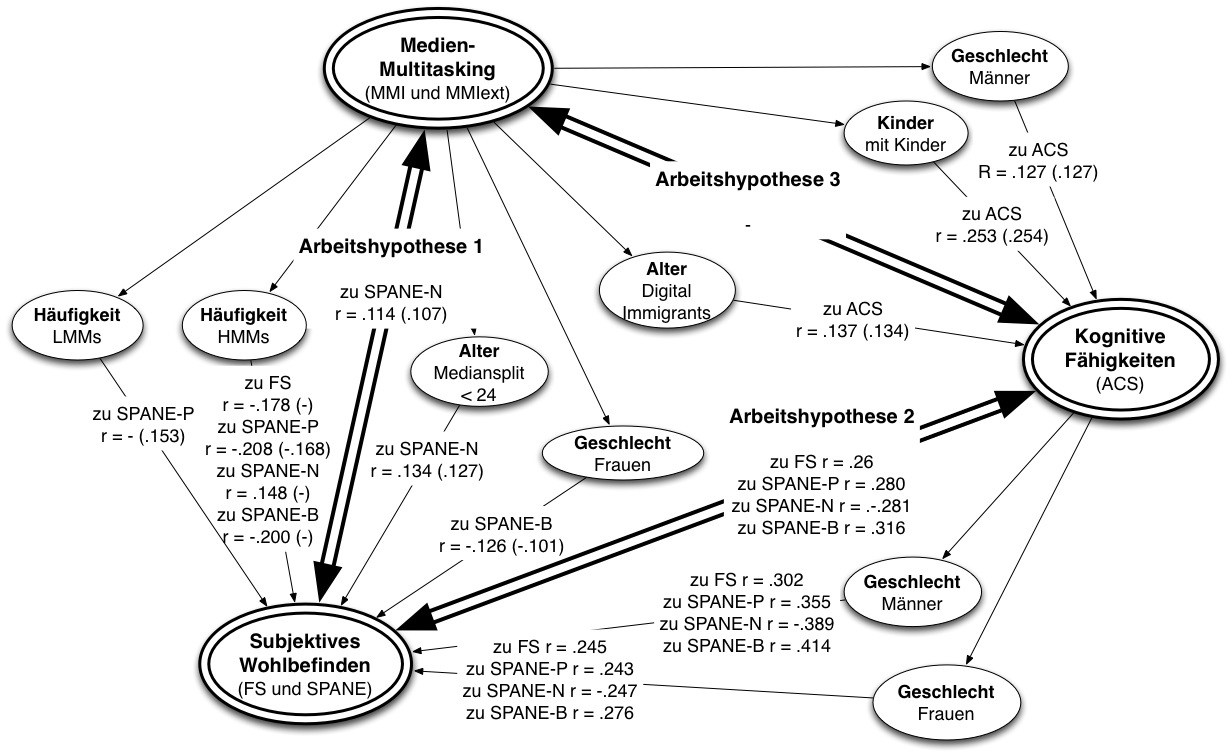
\includegraphics[scale=0.5, angle=90]{images/grafiken/Zusammenhang_Zusammenfassung_v2.jpg}
     \caption{Zusammenfassende Ergebnisse der Variablen gross}
     \label{pic.ergebniss.zusammenfassungGross}
\end{figure}

\end{RaggedRight}


%%%%%%%%%%%%%%%%%%%%%%%%%%%%%%%%%%%%%%%%%%%%%%%%%%%%%%%%%%%%% 
%% Schlussblatt
%%%%%%%%%%%%%%%%%%%%%%%%%%%%%%%%%%%%%%%%%%%%%%%%%%%%%%%%%%%%%
% Blatt mit Unterschrift

\includepdf{images/Bachelorarbeit_Unterschrift.pdf}

\end{document}
